\documentclass[12pt, a4paper, simple]{eskdtext}

\usepackage{config/main.env}
\usepackage{config/report.env}
\usepackage{styles/listing}
\usepackage{styles/lists}
\usepackage{styles/SectionMargins}
\usepackage{styles/table}
\usepackage{styles/TableOfContent}
\usepackage{styles/url}

\begin{document}
  \begin{ESKDtitlePage}
  \ESKDstyle{empty}
  \begin{center}
    \envReportMinistr \\
    \envReportEducation \\
    \envReportUniversity \\
    \envReportCathedra \\
  \end{center}

  \vfill

  \begin{center}
    Тема: <<\envReportTitle>>
  \end{center}

  \vfill

  \begin{center}
    Отчёт лабораторной работы №\envReportLabNumber \\
    по дисциплине \envReportSubject \\
  \end{center}

  \vfill

  \begin{flushright}
    \begin{minipage}[t]{7cm}
      Выполнил: \\
      \envReportStudentInfo \\
      \hspace{0pt} \\
      Проверил: \\
      \envReportTeacherInfo \\
    \end{minipage}
  \end{flushright}

  \vfill

  \begin{center}
    \envReportCity~\ESKDtheYear
  \end{center}
\end{ESKDtitlePage}


  % = = = = = = = = = = = = = = = =
  \ESKDstyle{empty}
  \begin{center}
    \textbf{Отчёт лабораторной работы №\envReportLabNumber}
  \end{center}

  \paragraph{} \textbf{Тема}: <<\envReportTitle>>

  \paragraph{} \textbf{Цель}:
  Знакомство с Cloud Functions, Cloud Scheduler, BigTable, BigQuery.

  \paragraph{} \textbf{Что нужно сделать}:

  Напишите микросервис MS4, имитирующий действия пользователя, который вызывает разные API сервиса MS2 при помощи обычных HTTP запросов. 
  
  Сервис MS4 должен быть запущен при помощи serverless платформы Cloud Functions. 
  
  Каждый раз, когда функция выполняется, она должна случайным образом образом решить – какое действие выполнять и выполнять ли его в этот конкретный раз, тем самым получив случайное распределение действий пользователя.
  
  % Триггер для выполнения функции – Pub/Sub. Запланируйте job в Cloud Scheduler, который будет раз в минуту писать в соответствующий топик Pub/Sub.

  Запланируйте job в Cloud Scheduler, который будет раз в минуту запускать Google Cloud Functions.
  
  Результаты выполнения своих действий функция должна записывать в BigTable. Используя BigQuery, покажите данные результаты (несколько разных запросов BigQuery).
  
  \paragraph{} \textbf{Ход работы}:

  \begin{center}
    \textbf{Создание Google Cloud BigTable}
  \end{center}

  Заходим на сайт Google Cloud Console \cite{GoogleCloudConsole} (см. рисунок~\ref{fig:1}).

  Menu > Bigtable \cite{GoogleCloudBigTable} (см. рисунок~\ref{fig:1}).

  \begin{figure}[!h]
    \centering
    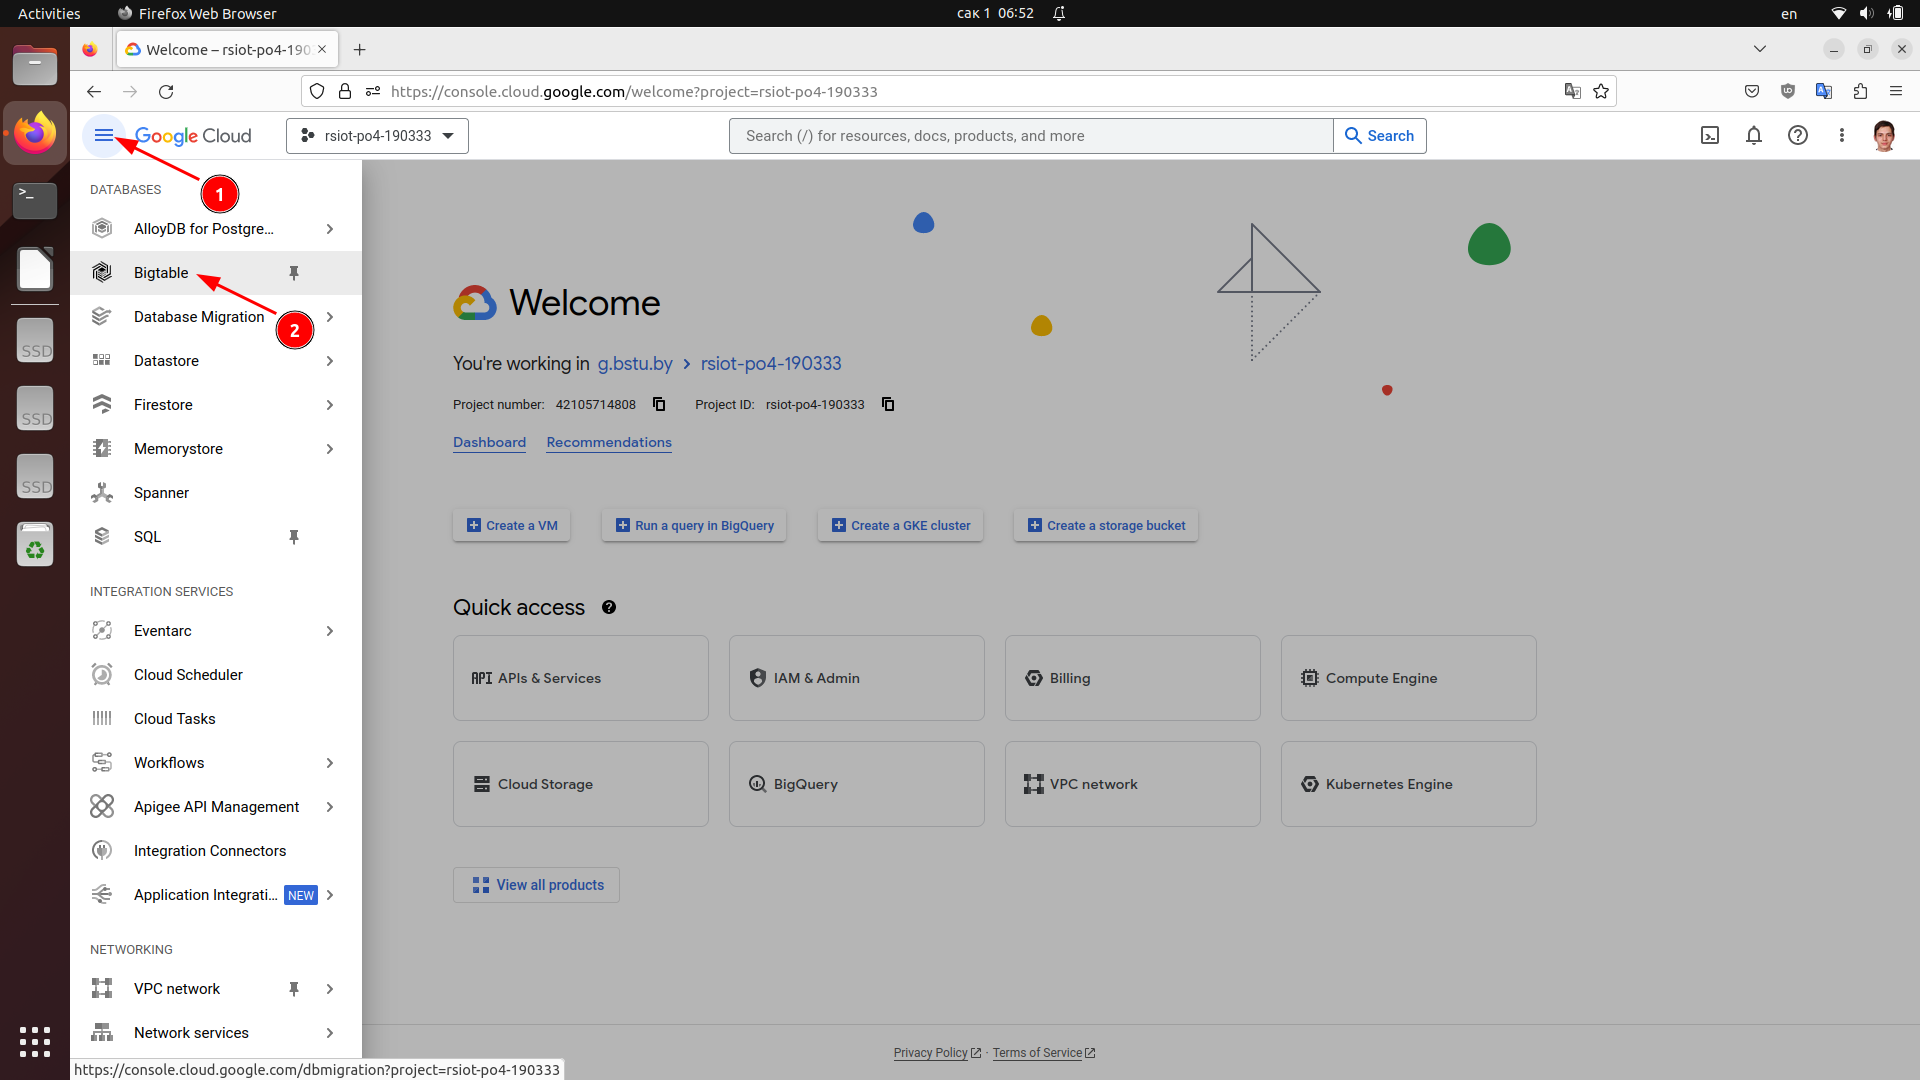
\includegraphics[width=11cm]
    {images/GoogleCloudBigTable/2023-03-01_06-52-29.png}
    \caption{\_}
    \label{fig:1}
  \end{figure}

  Жму <<CREATE INSTANCE>> (см. рисунок~\ref{fig:2}).

  \begin{figure}[!h]
    \centering
    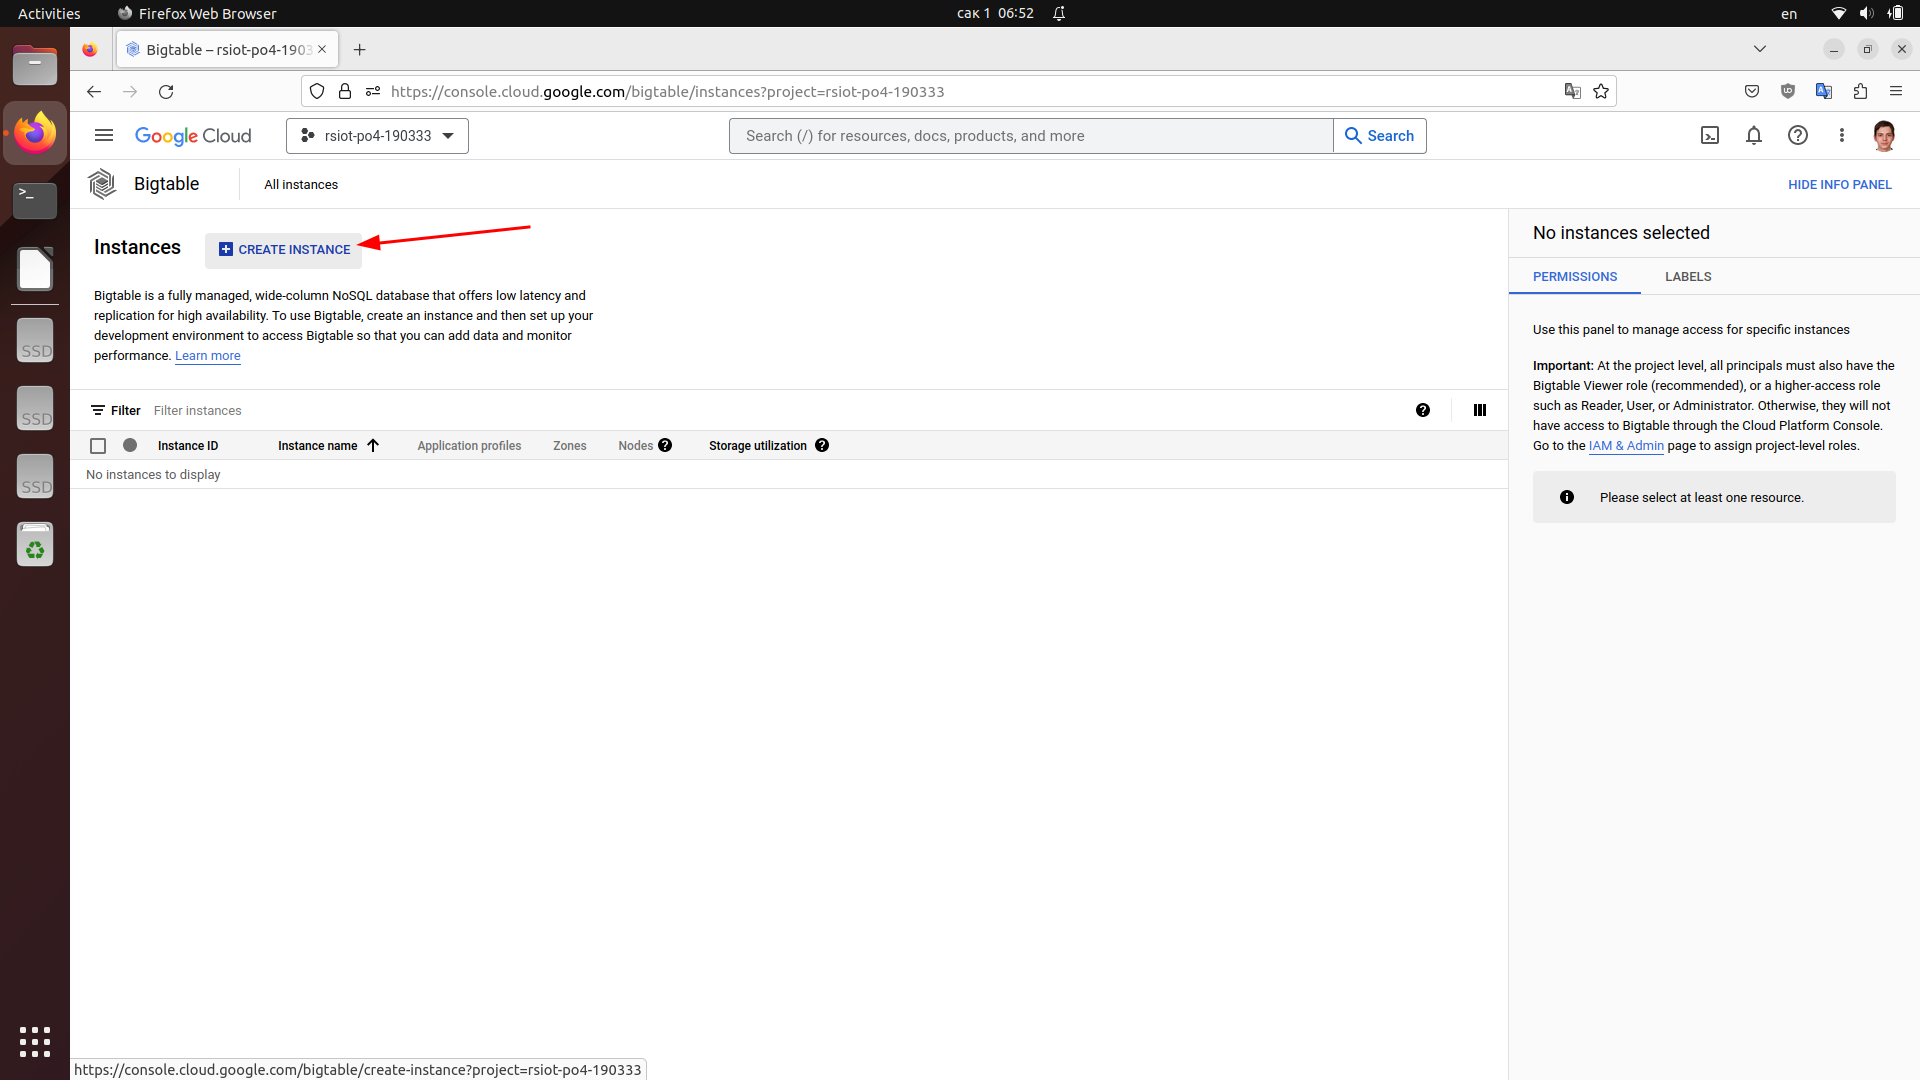
\includegraphics[width=11cm]
    {images/GoogleCloudBigTable/2023-03-01_06-53-01.png}
    \caption{\_}
    \label{fig:2}
  \end{figure}

  \newpage

  Instance name: \underline{rsiot-po4-190333-bigtable} (см. рисунок~\ref{fig:3}).
  
  % Instance ID: \underline{rsiot-po4-190333-bigtable} (см. рисунок~\ref{fig:3}).

  Жму <<HIDE DETAILS>> (см. рисунок~\ref{fig:3}).

  Try another storage size: \underline{1 GB} (см. рисунок~\ref{fig:3}). Жму <<CONTINUE>> (см. рисунок~\ref{fig:3}).

  \begin{figure}[!h]
    \centering
    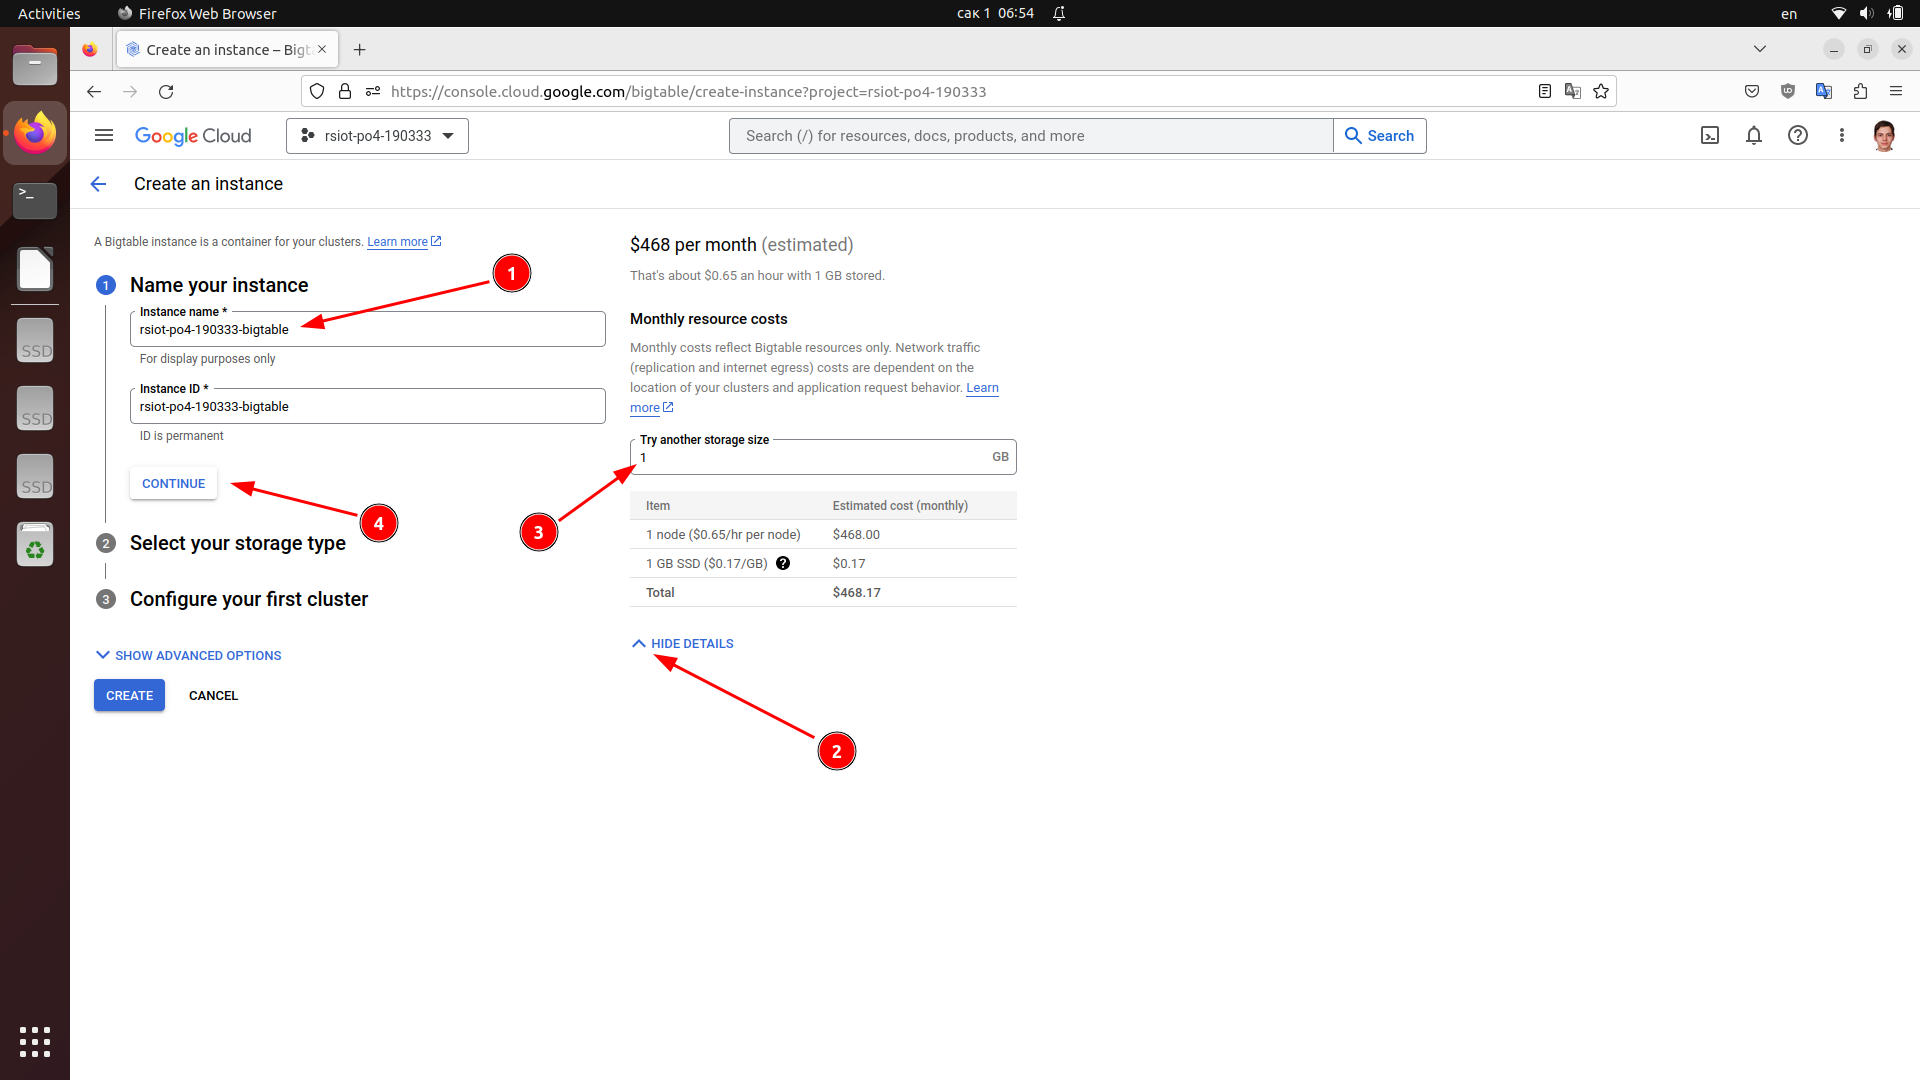
\includegraphics[width=11cm]
    {images/GoogleCloudBigTable/2023-03-01_06-55-06.png}
    \caption{\_}
    \label{fig:3}
  \end{figure}

  Select yout storage type: \underline{HDD} (см. рисунок~\ref{fig:4}).

  Жму <<CONTINUE>> (см. рисунок~\ref{fig:4}).

  \begin{figure}[!h]
    \centering
    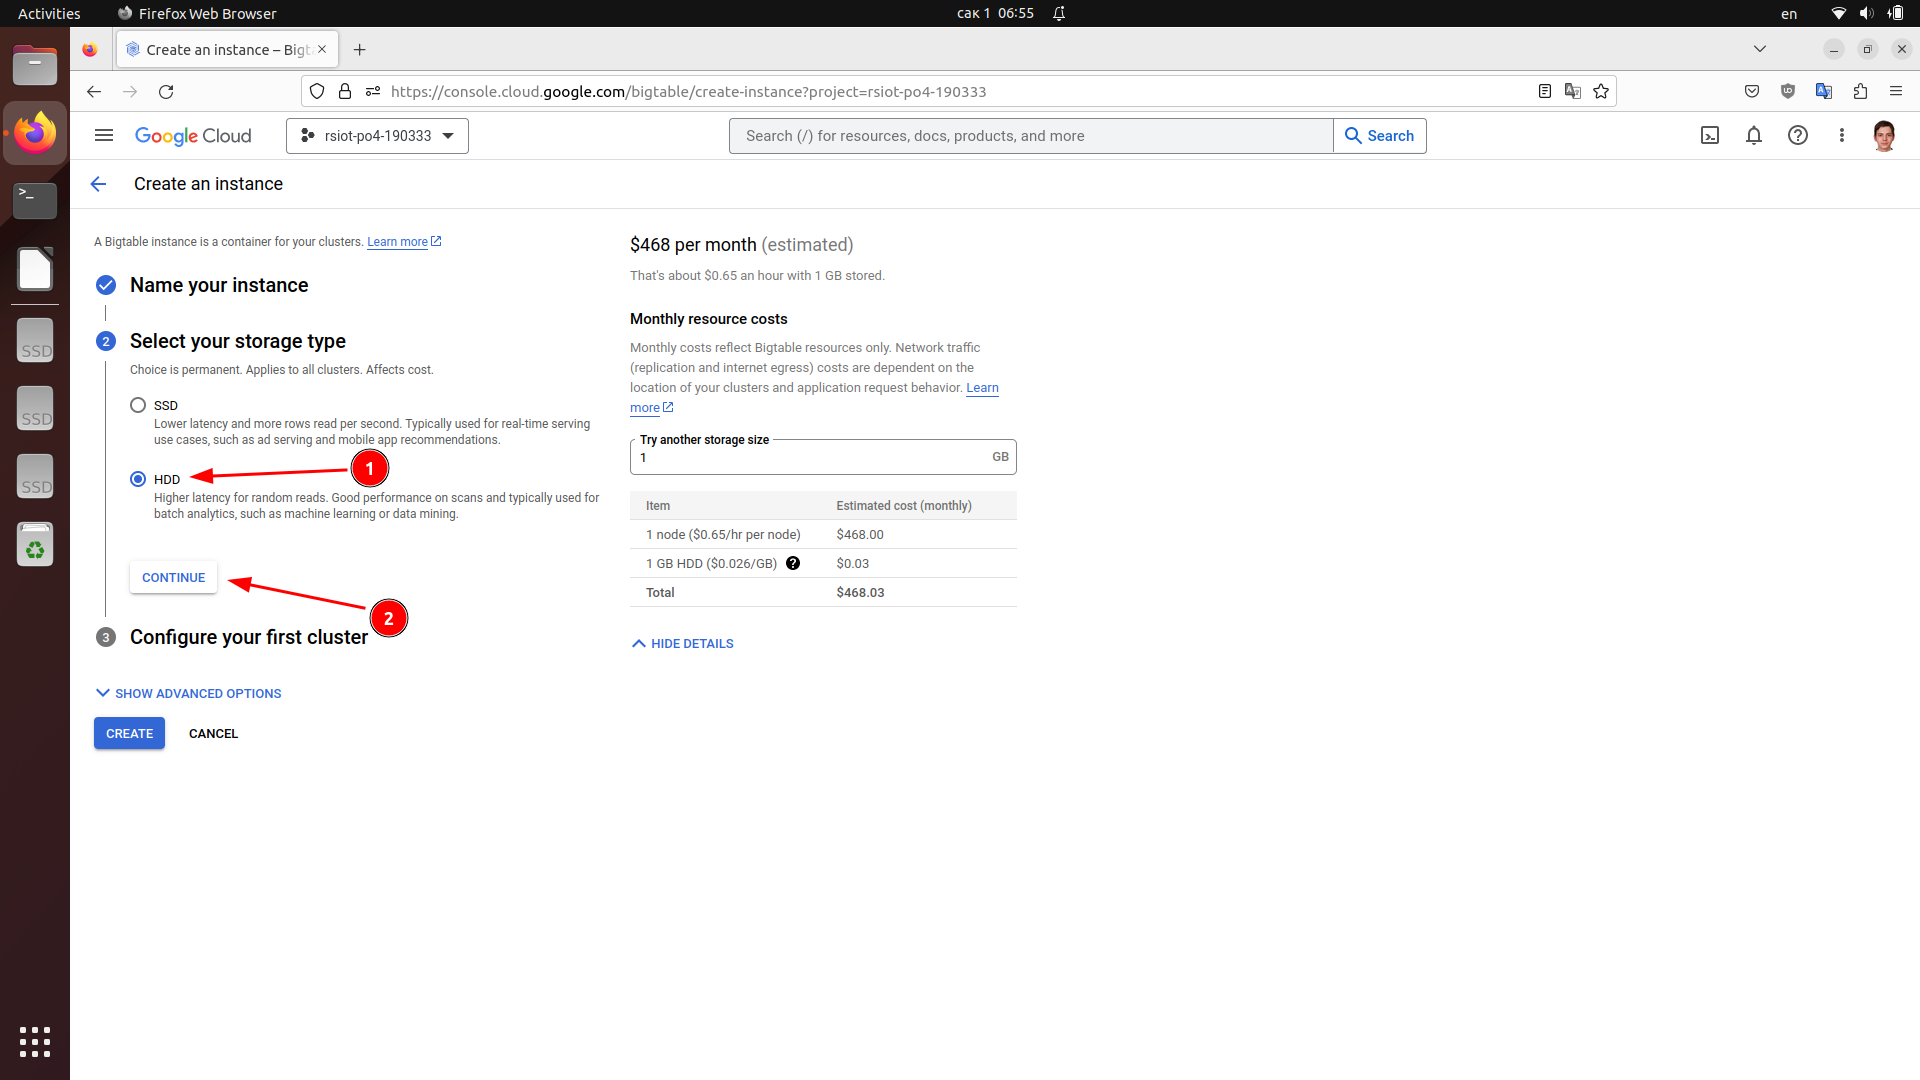
\includegraphics[width=11cm]
    {images/GoogleCloudBigTable/2023-03-01_06-55-34.png}
    \caption{\_}
    \label{fig:4}
  \end{figure}

  \newpage

  Region: \underline{us-central1 (lowa)} (см. рисунок~\ref{fig:5}).

  Жму <<CREATE>> (см. рисунок~\ref{fig:5}).

  \begin{figure}[!h]
    \centering
    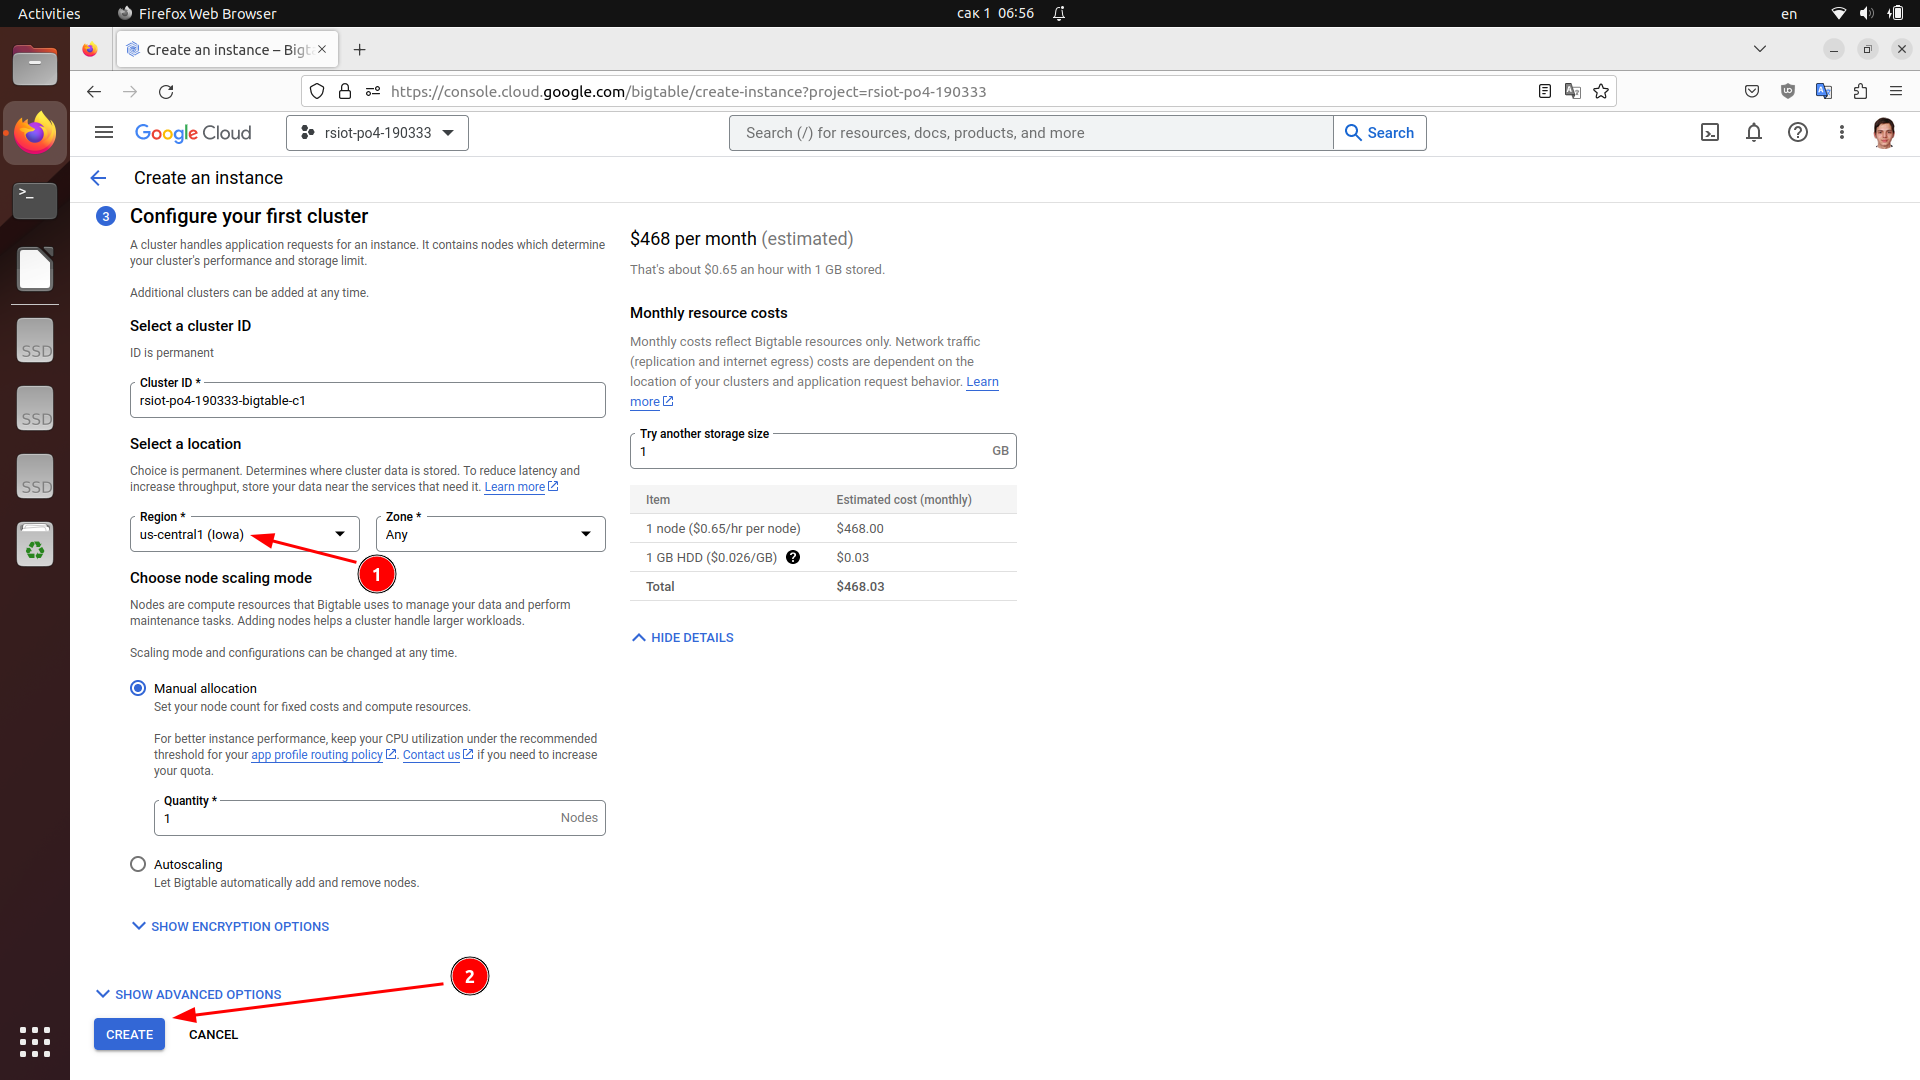
\includegraphics[width=11cm]
    {images/GoogleCloudBigTable/2023-03-01_06-56-40.png}
    \caption{\_}
    \label{fig:5}
  \end{figure}

  Жму по instance ID <<rsiot-po4-190333-bigtable>> (см. рисунок~\ref{fig:6}).

  \begin{figure}[!h]
    \centering
    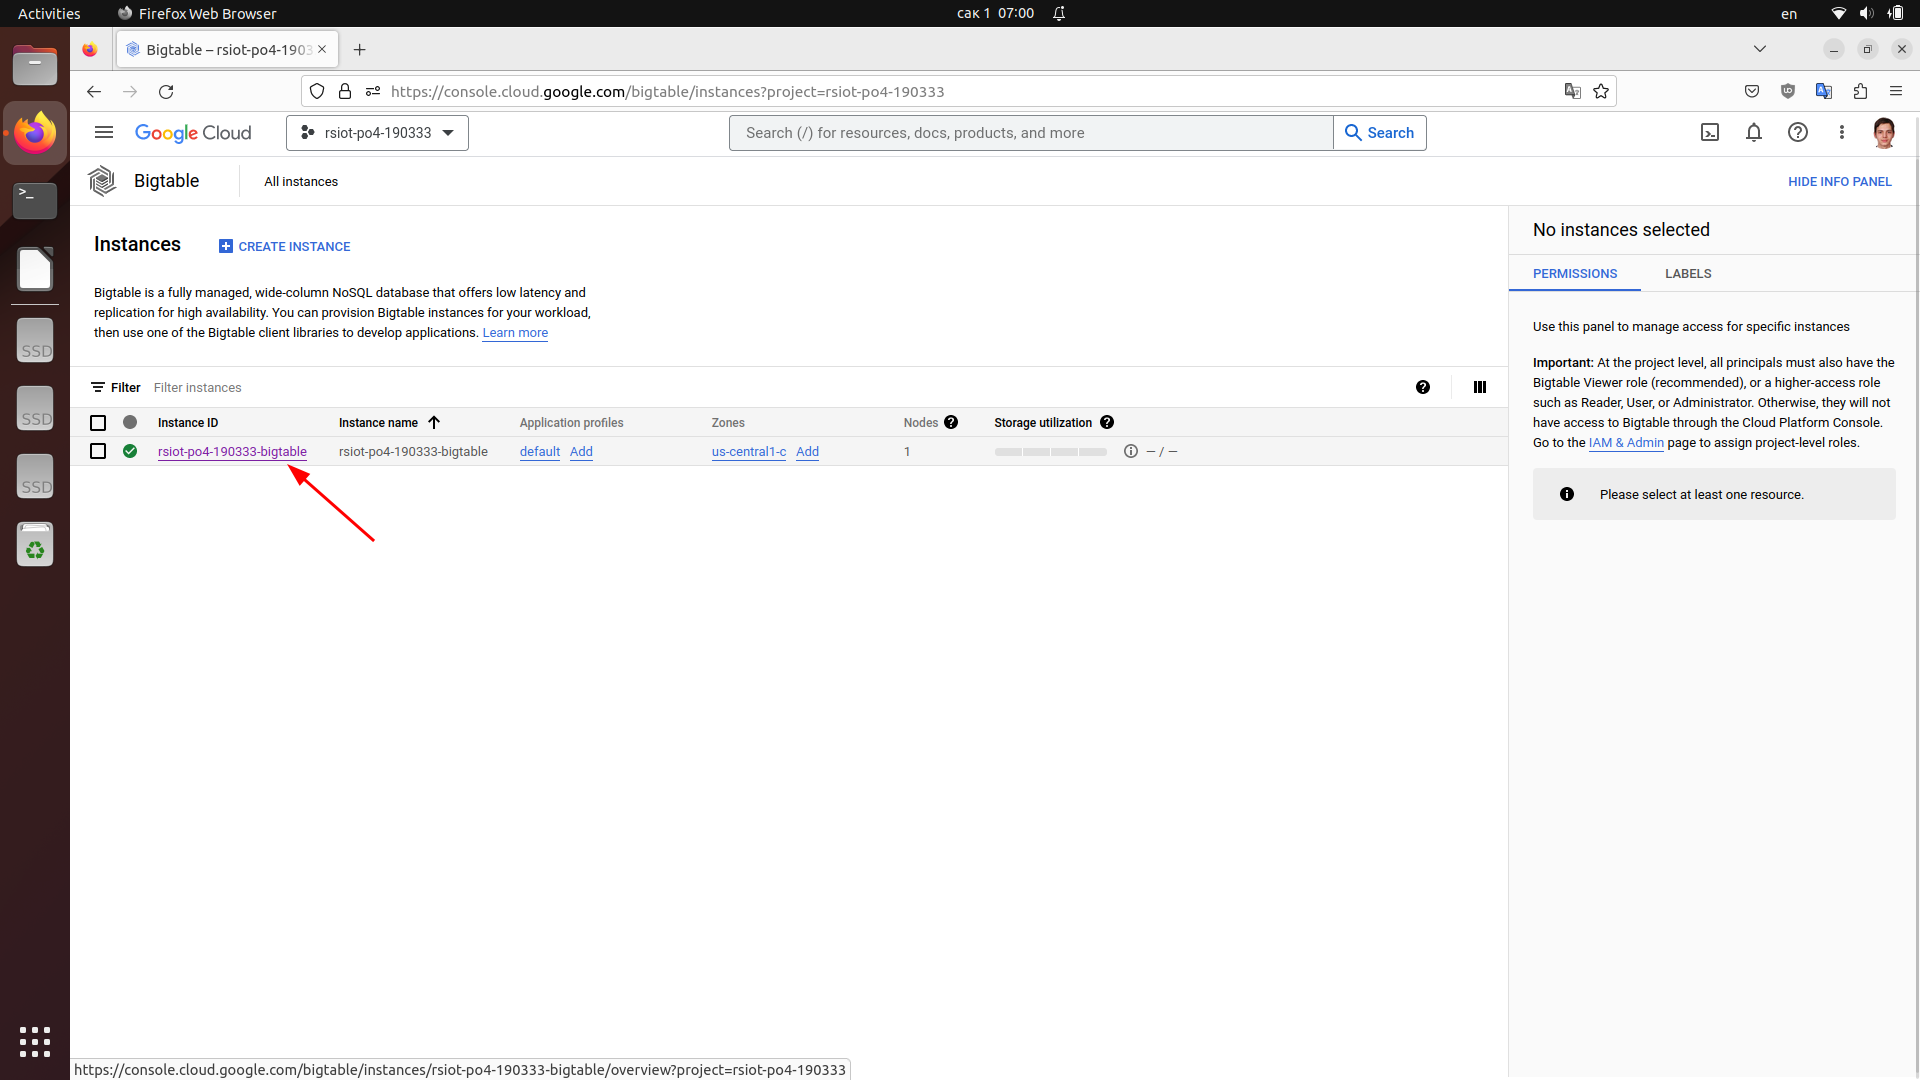
\includegraphics[width=11cm]
    {images/GoogleCloudBigTable/2023-03-01_07-00-22.png}
    \caption{\_}
    \label{fig:6}
  \end{figure}

  Жму <<Tables>> (см. рисунок~\ref{fig:7}).

  Жму <<CREATE TABLE>> (см. рисунок~\ref{fig:7}).

  Table ID: \underline{rsiot-po4-190333-bigtable} (см. рисунок~\ref{fig:7}).

  Жму <<ADD COLUMN FAMILY>> (см. рисунок~\ref{fig:7}).

  Column family name: \underline{column-family-name} (см. рисунок~\ref{fig:7}).

  Жму <<DONE>> (см. рисунок~\ref{fig:7}).

  Жму <<CREATE>> (см. рисунок~\ref{fig:7}).

  Созданныя таблица изображена на рис.~\ref{fig:8}.

  \begin{figure}[!h]
    \centering
  
    \begin{minipage}{0.49\textwidth}
      \centering
  
      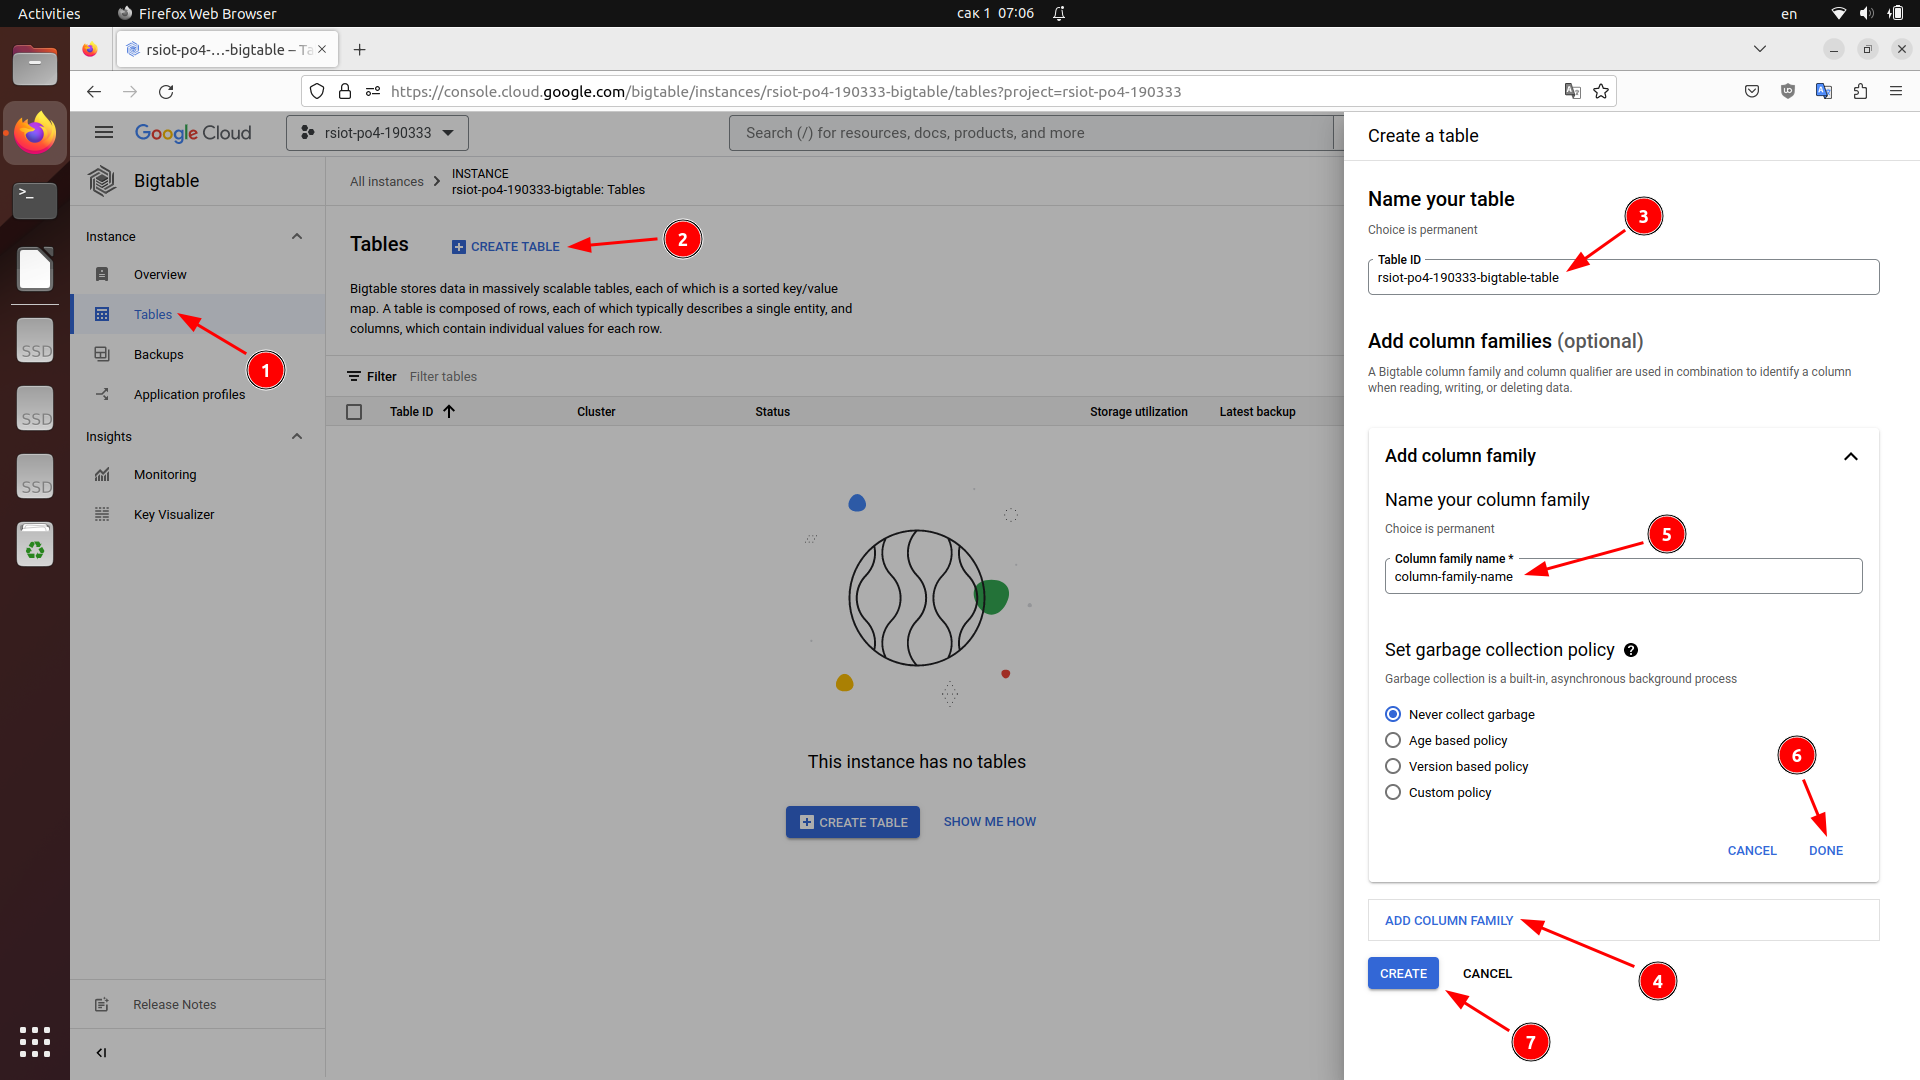
\includegraphics[height=5cm]
      {images/GoogleCloudBigTable/2023-03-01_07-07-28.png}
  
      \caption{\_}
  
      \label{fig:7}
    \end{minipage}
    \begin{minipage}{0.49\textwidth}
      \centering
  
      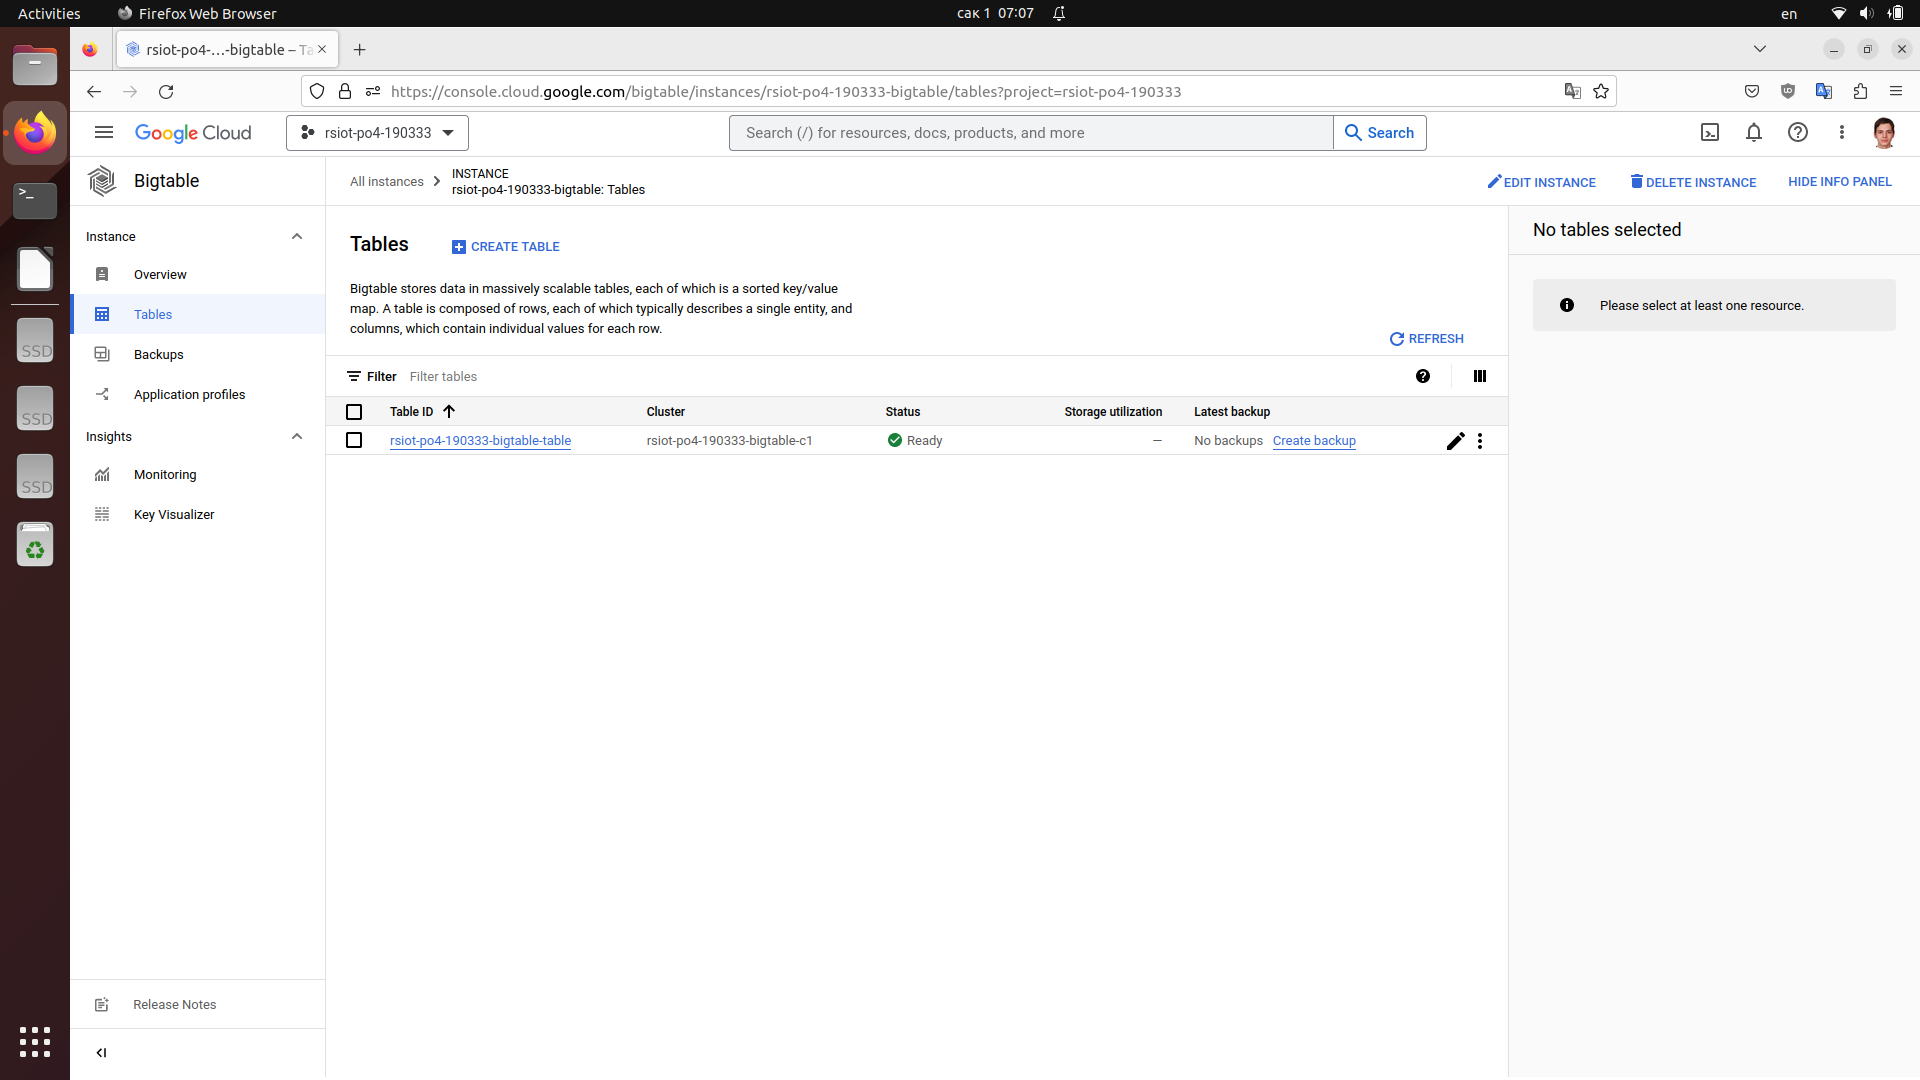
\includegraphics[height=5cm]
      {images/GoogleCloudBigTable/2023-03-01_07-07-46.png}
  
      \caption{\_}
  
      \label{fig:8}
    \end{minipage}
  \end{figure}

  \newpage
  \begin{center}
    \textbf{Создание сервисного аккаунта для Google Cloud BigTable}
  \end{center}

  Заходим на сайт Google Cloud Console \cite{GoogleCloudConsole} (см. рисунок~\ref{fig:9}).

  Menu > IAM \& Admin > Service Accounts \cite{GoogleCloudServiceAccounts} (см. рисунок~\ref{fig:9}).

  \begin{figure}[!h]
    \centering
    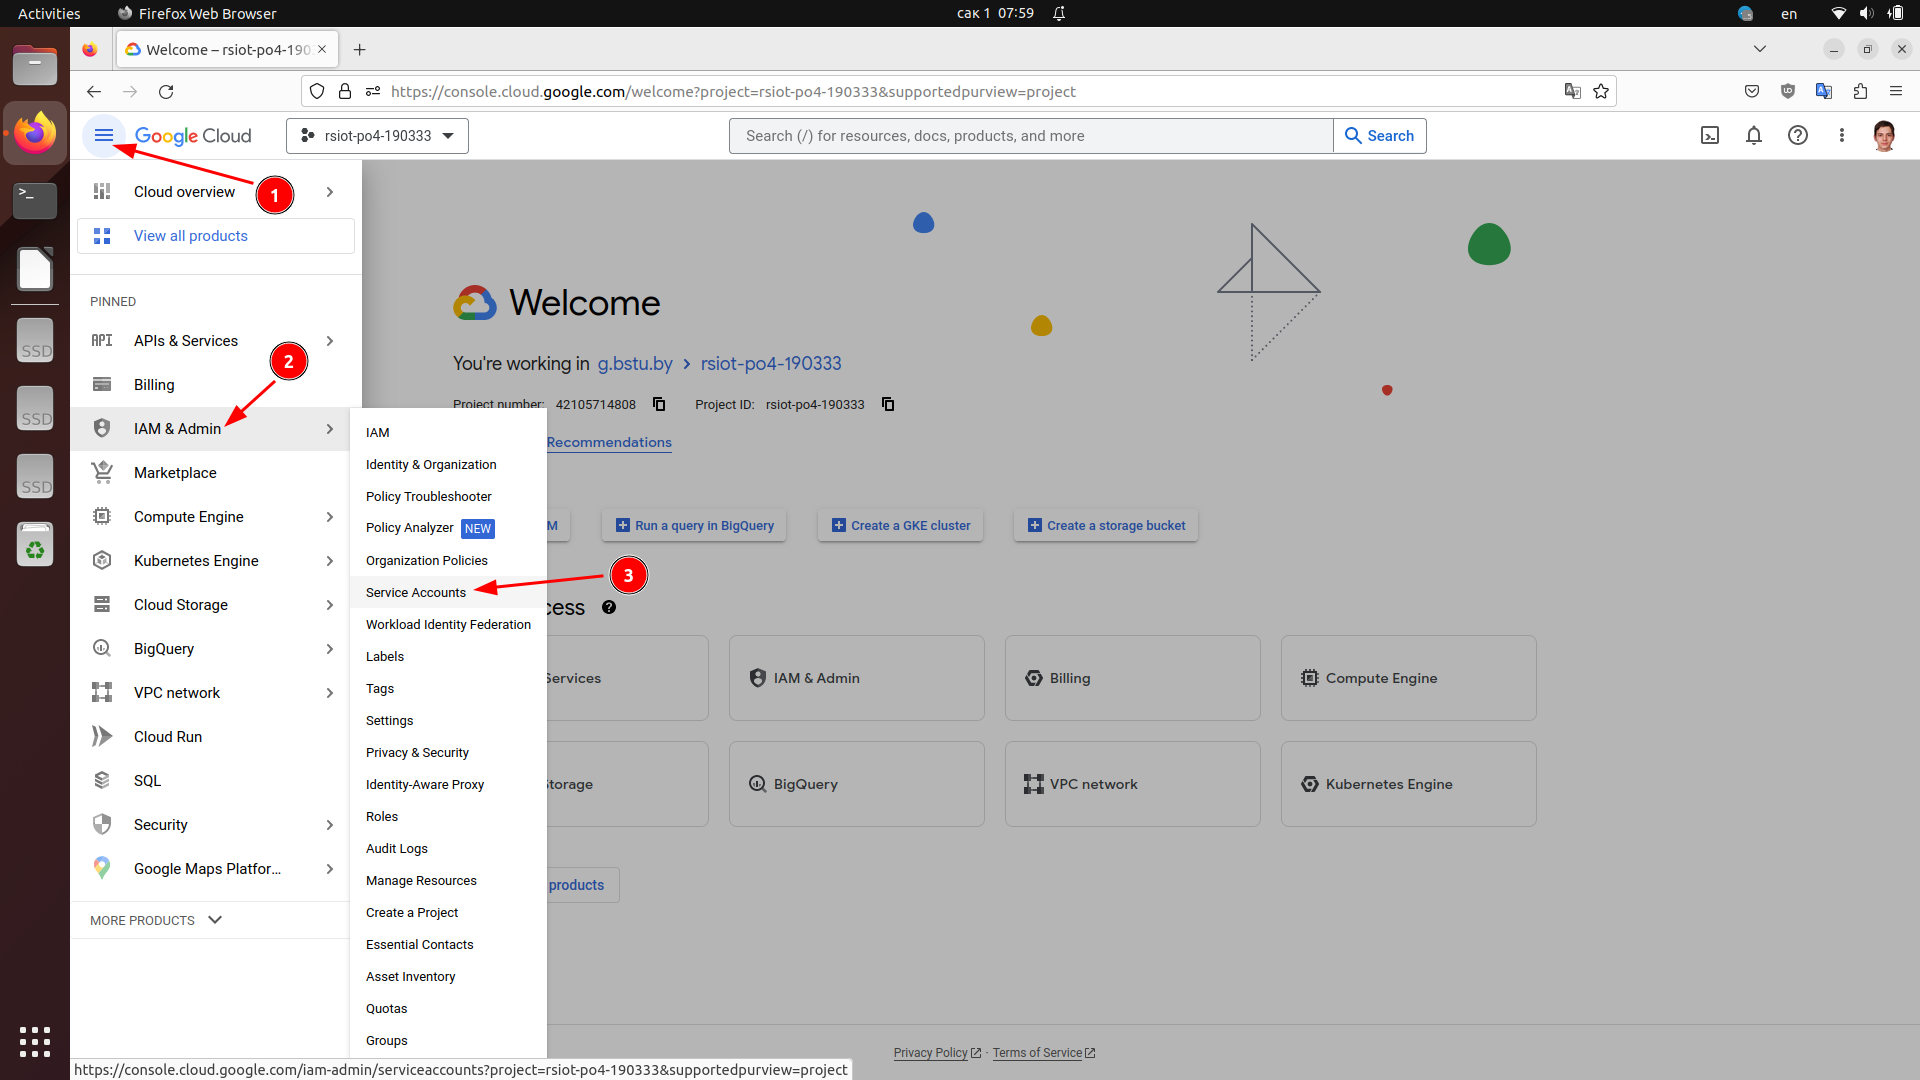
\includegraphics[width=11cm]
    {images/GoogleCloudBigTable/2023-03-01_07-59-42.png}
    \caption{\_}
    \label{fig:9}
  \end{figure}

  Жму <<CREATE SERVICE ACCOUNT>> (см. рисунок~\ref{fig:10}).

  \begin{figure}[!h]
    \centering
    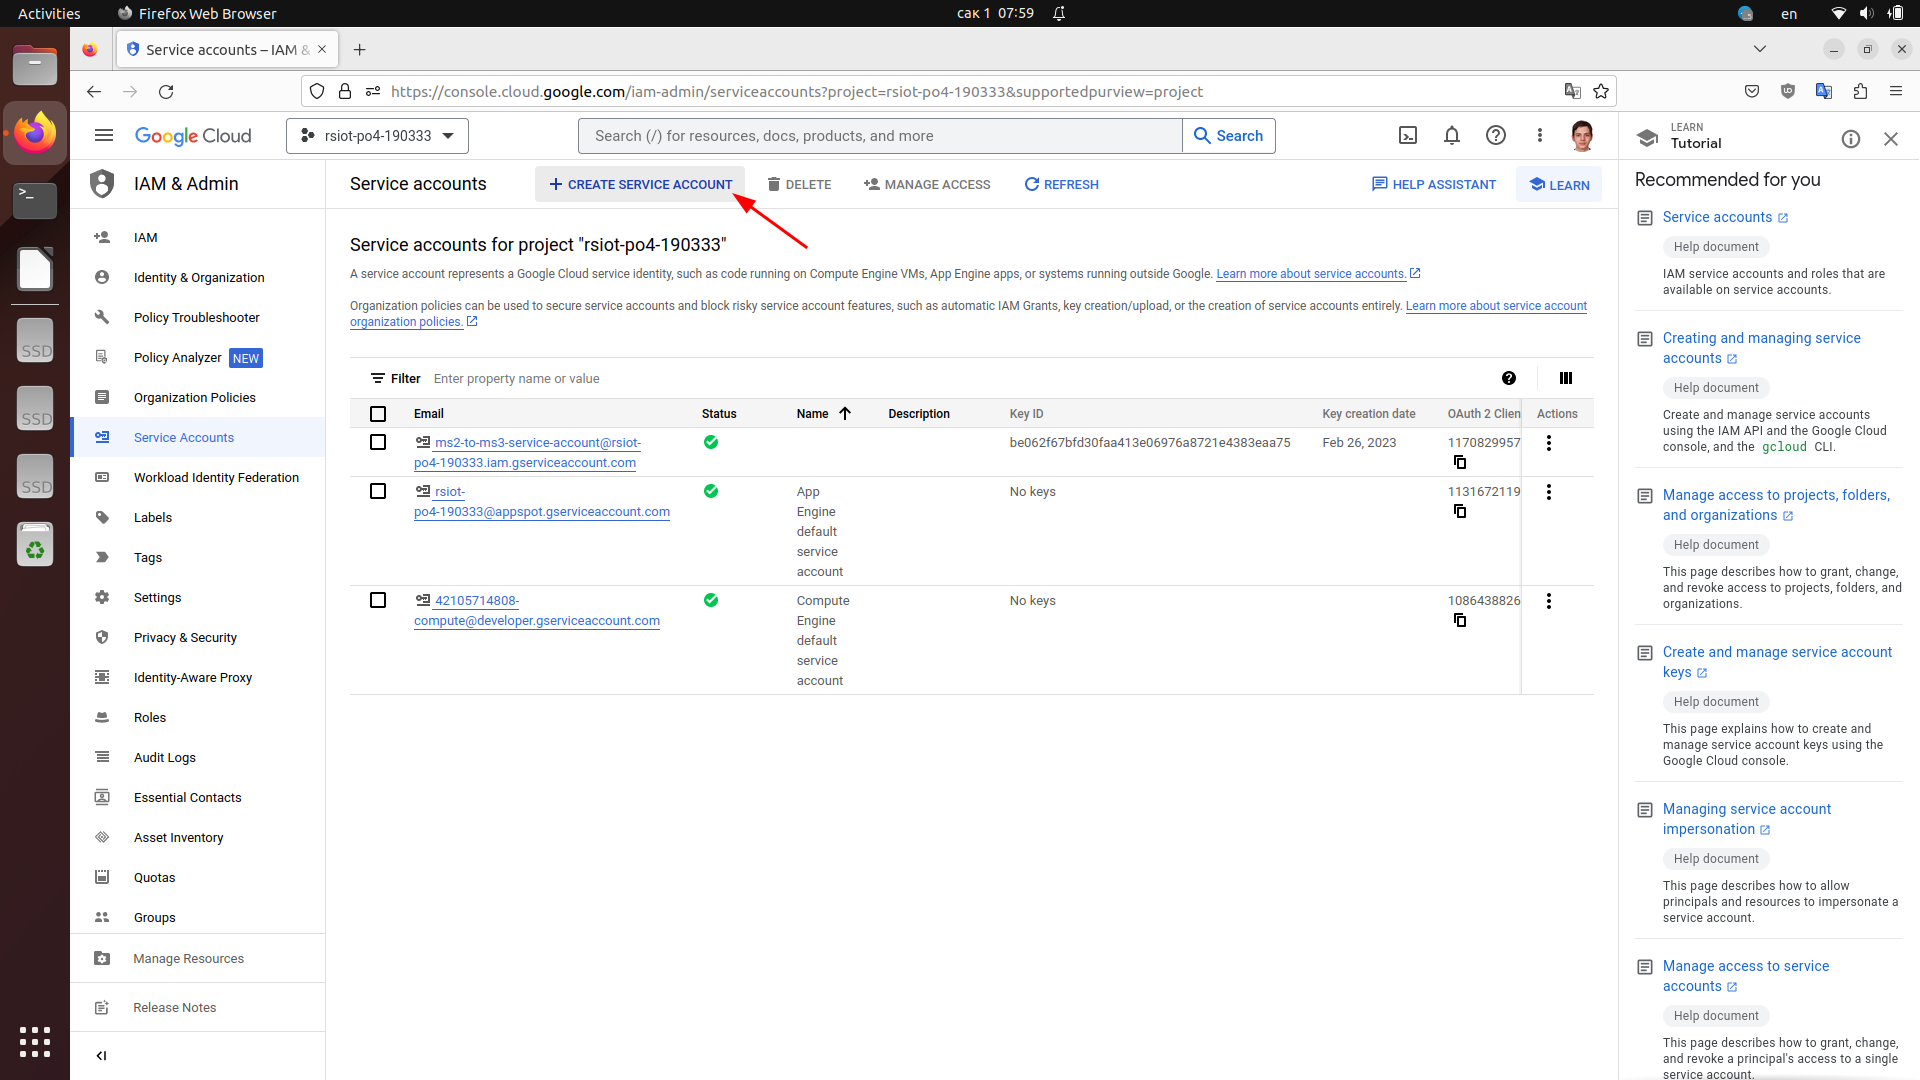
\includegraphics[width=11cm]
    {images/GoogleCloudBigTable/2023-03-01_08-00-04.png}
    \caption{\_}
    \label{fig:10}
  \end{figure}

  \newpage

  Service account ID: \underline{bigtable-service-account} (см. рисунок~\ref{fig:11}).

  Жму <<CREATE SERVICE ACCOUNT>> (см. рисунок~\ref{fig:11}).

  \begin{figure}[!h]
    \centering
    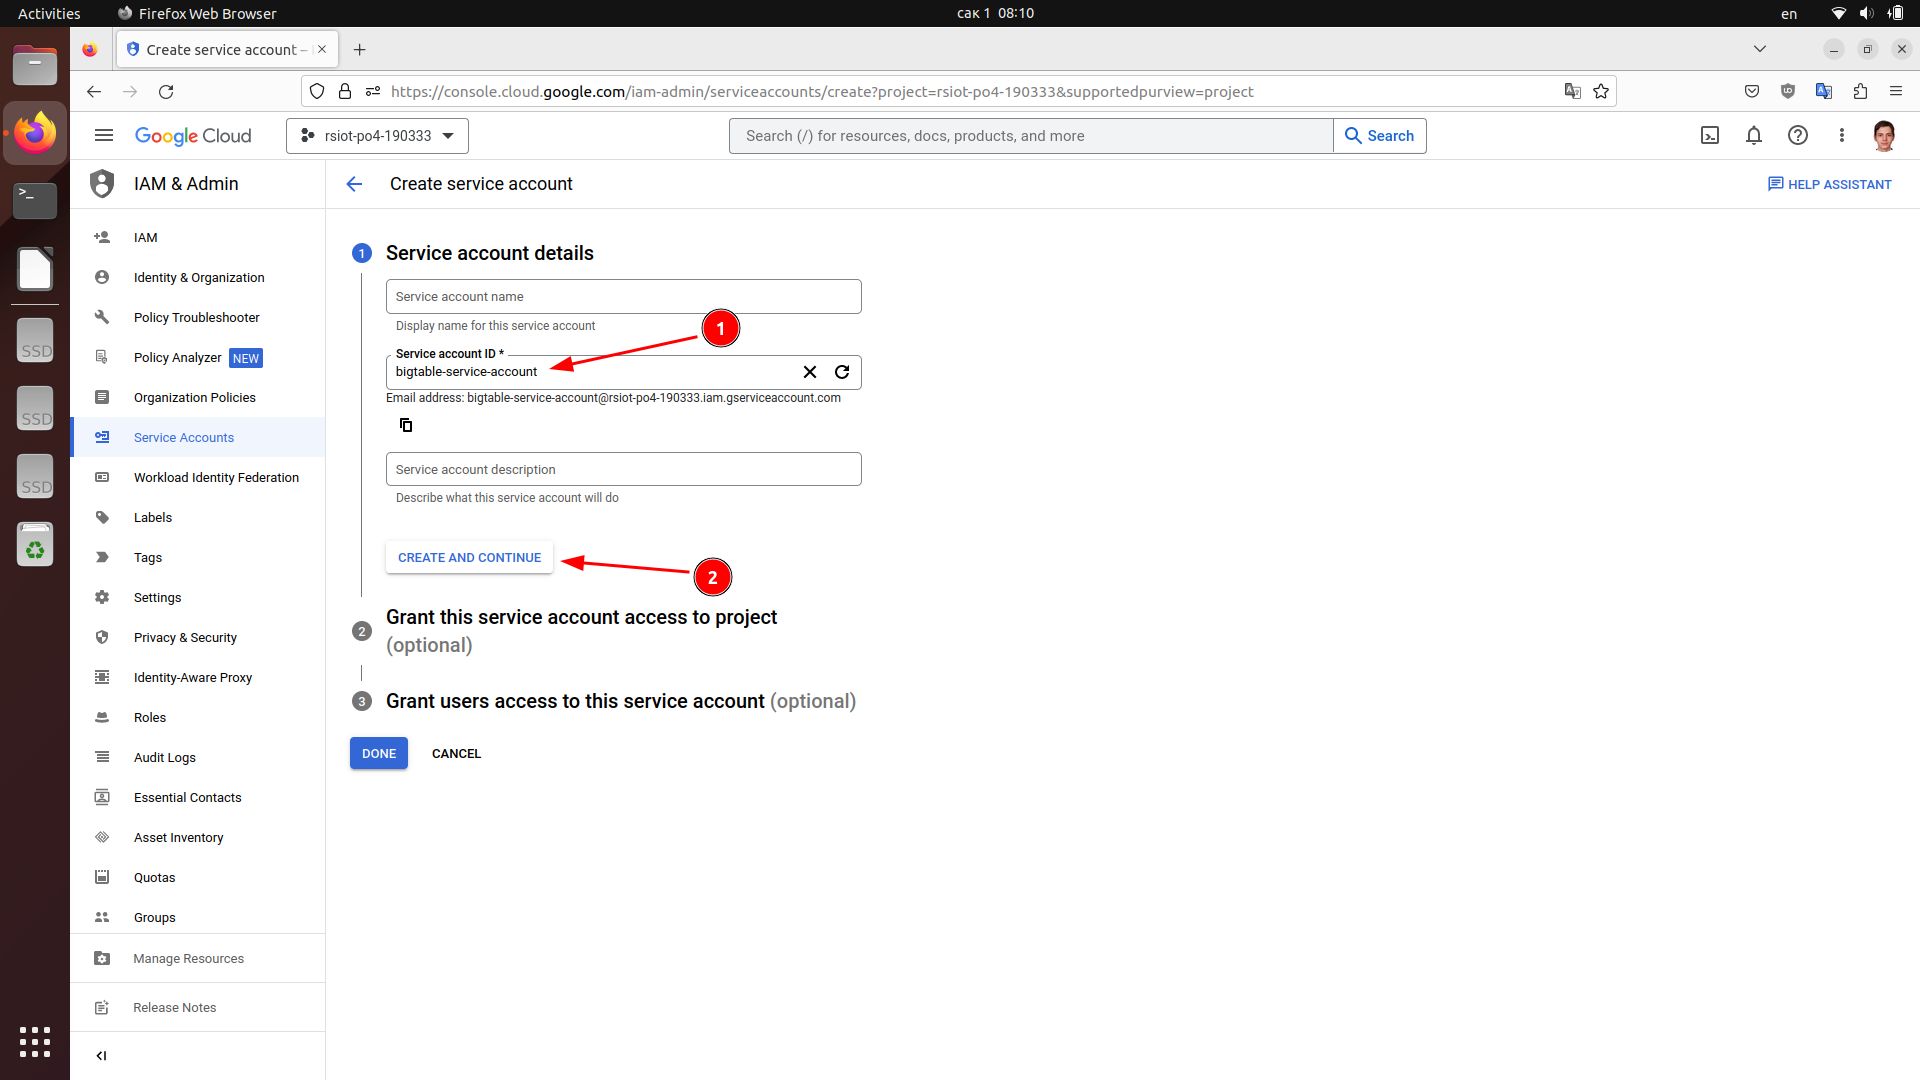
\includegraphics[width=11cm]
    {images/GoogleCloudBigTable/2023-03-01_08-10-44.png}
    \caption{\_}
    \label{fig:11}
  \end{figure}

  Жму Select a role > Cloud Bigtable > Bigtable Administrator (см. рисунок~\ref{fig:12}).

  Жму <<CONTINUE>> (см. рисунок~\ref{fig:12}).

  \begin{figure}[!h]
    \centering
    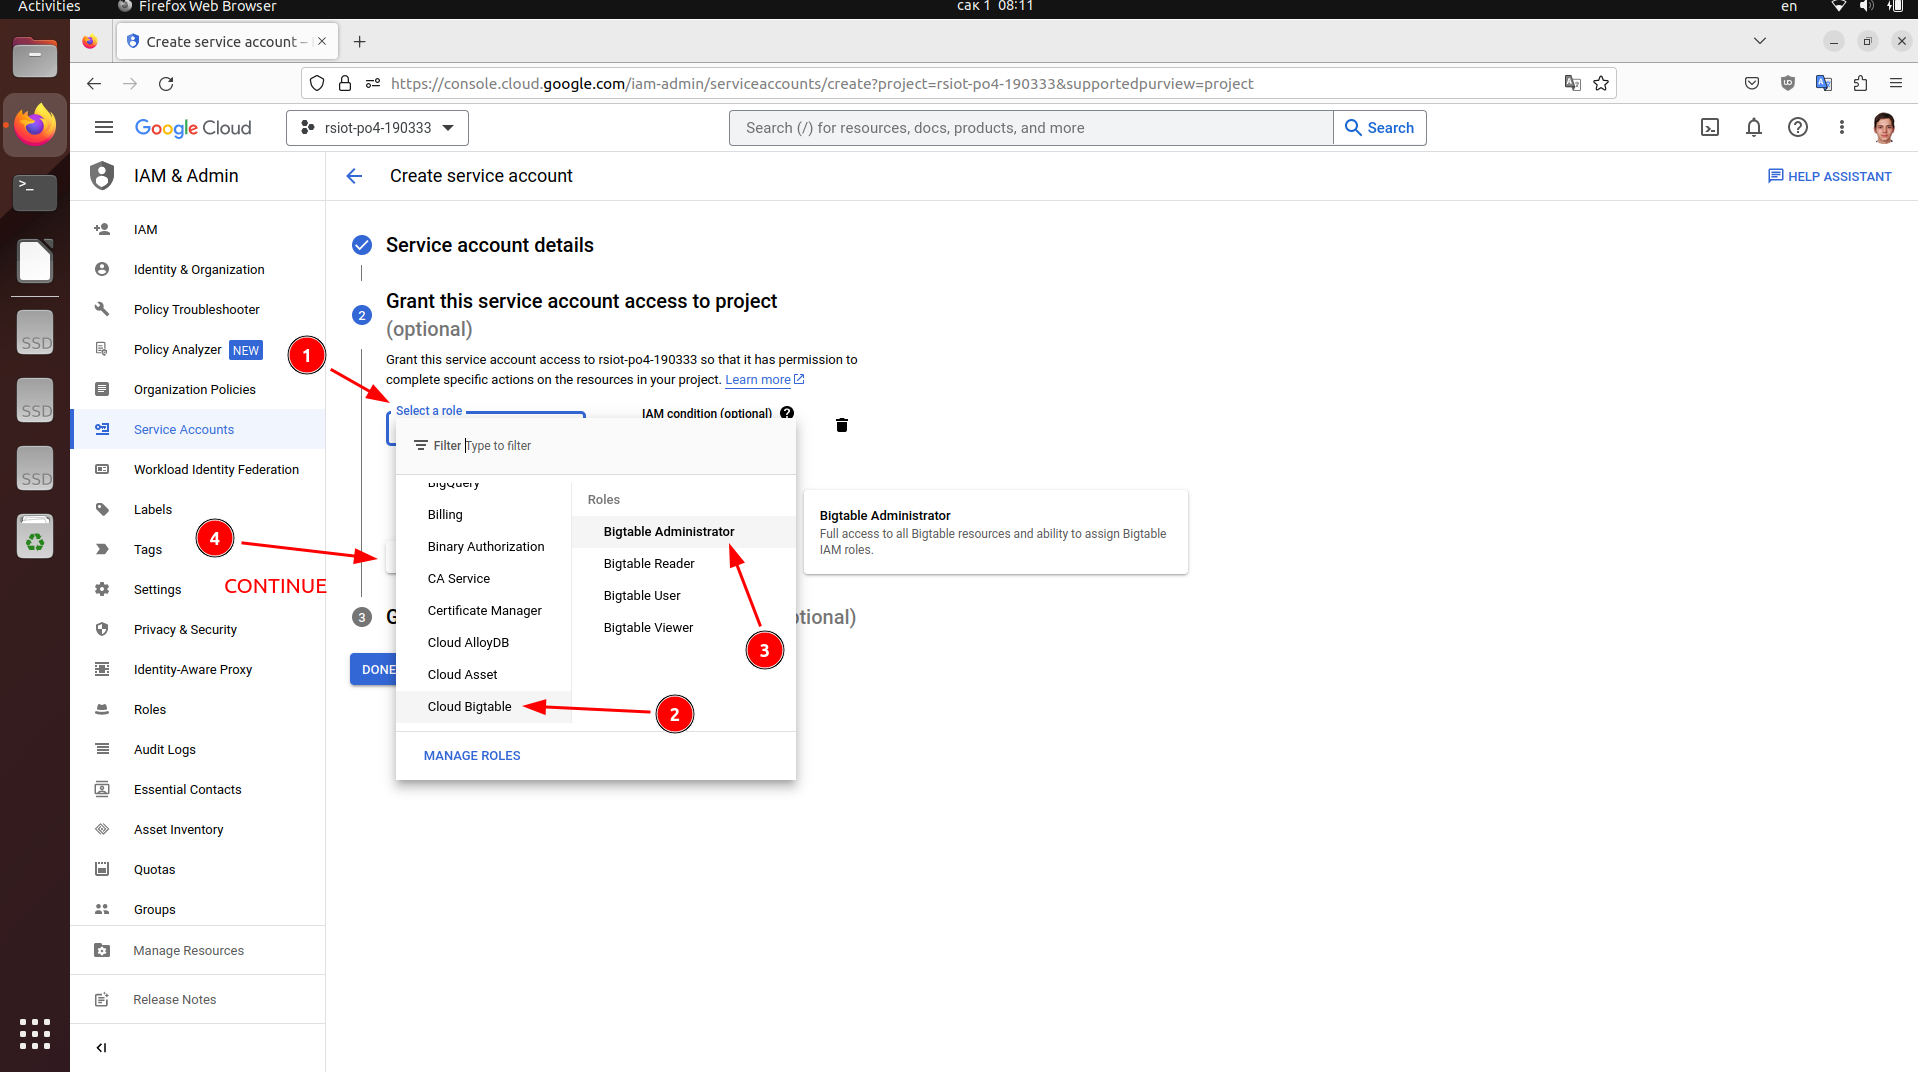
\includegraphics[width=11cm]
    {images/GoogleCloudBigTable/2023-03-01_08-12-32.png}
    \caption{\_}
    \label{fig:12}
  \end{figure}

  Жму <<DONE>> (см. рисунок~\ref{fig:13}).

  \begin{figure}[!h]
    \centering
    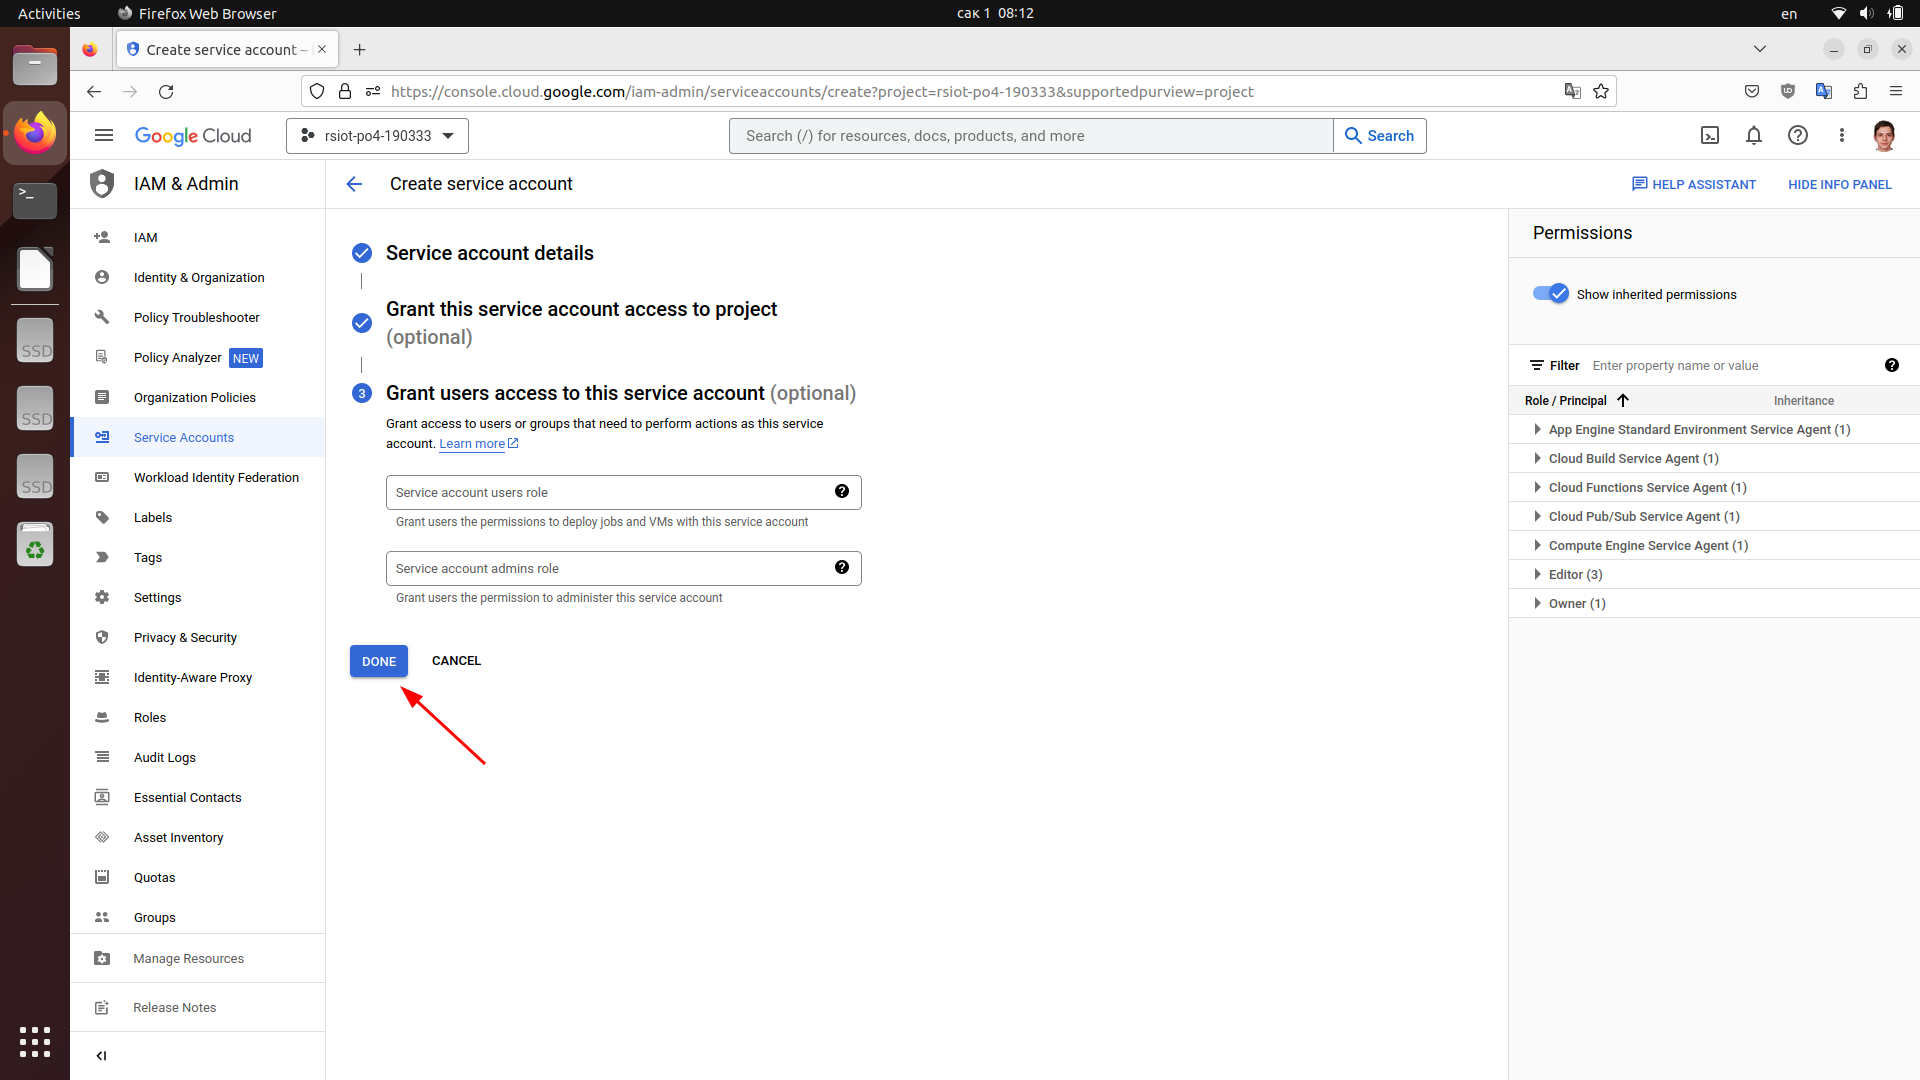
\includegraphics[width=10cm]
    {images/GoogleCloudBigTable/2023-03-01_08-12-57.png}
    \caption{\_}
    \label{fig:13}
  \end{figure}

  \newpage
  \begin{center}
    \textbf{Создание приватного ключа для Google Cloud BigTable}
  \end{center}

  Жму по почту сервисного аккаунта: \\
  \underline{bigtable-service-account@rsiot-po4-190333.iam.gserviceaccount.com} (см. рисунок~\ref{fig:14}).
  
  \begin{figure}[!h]
    \centering
    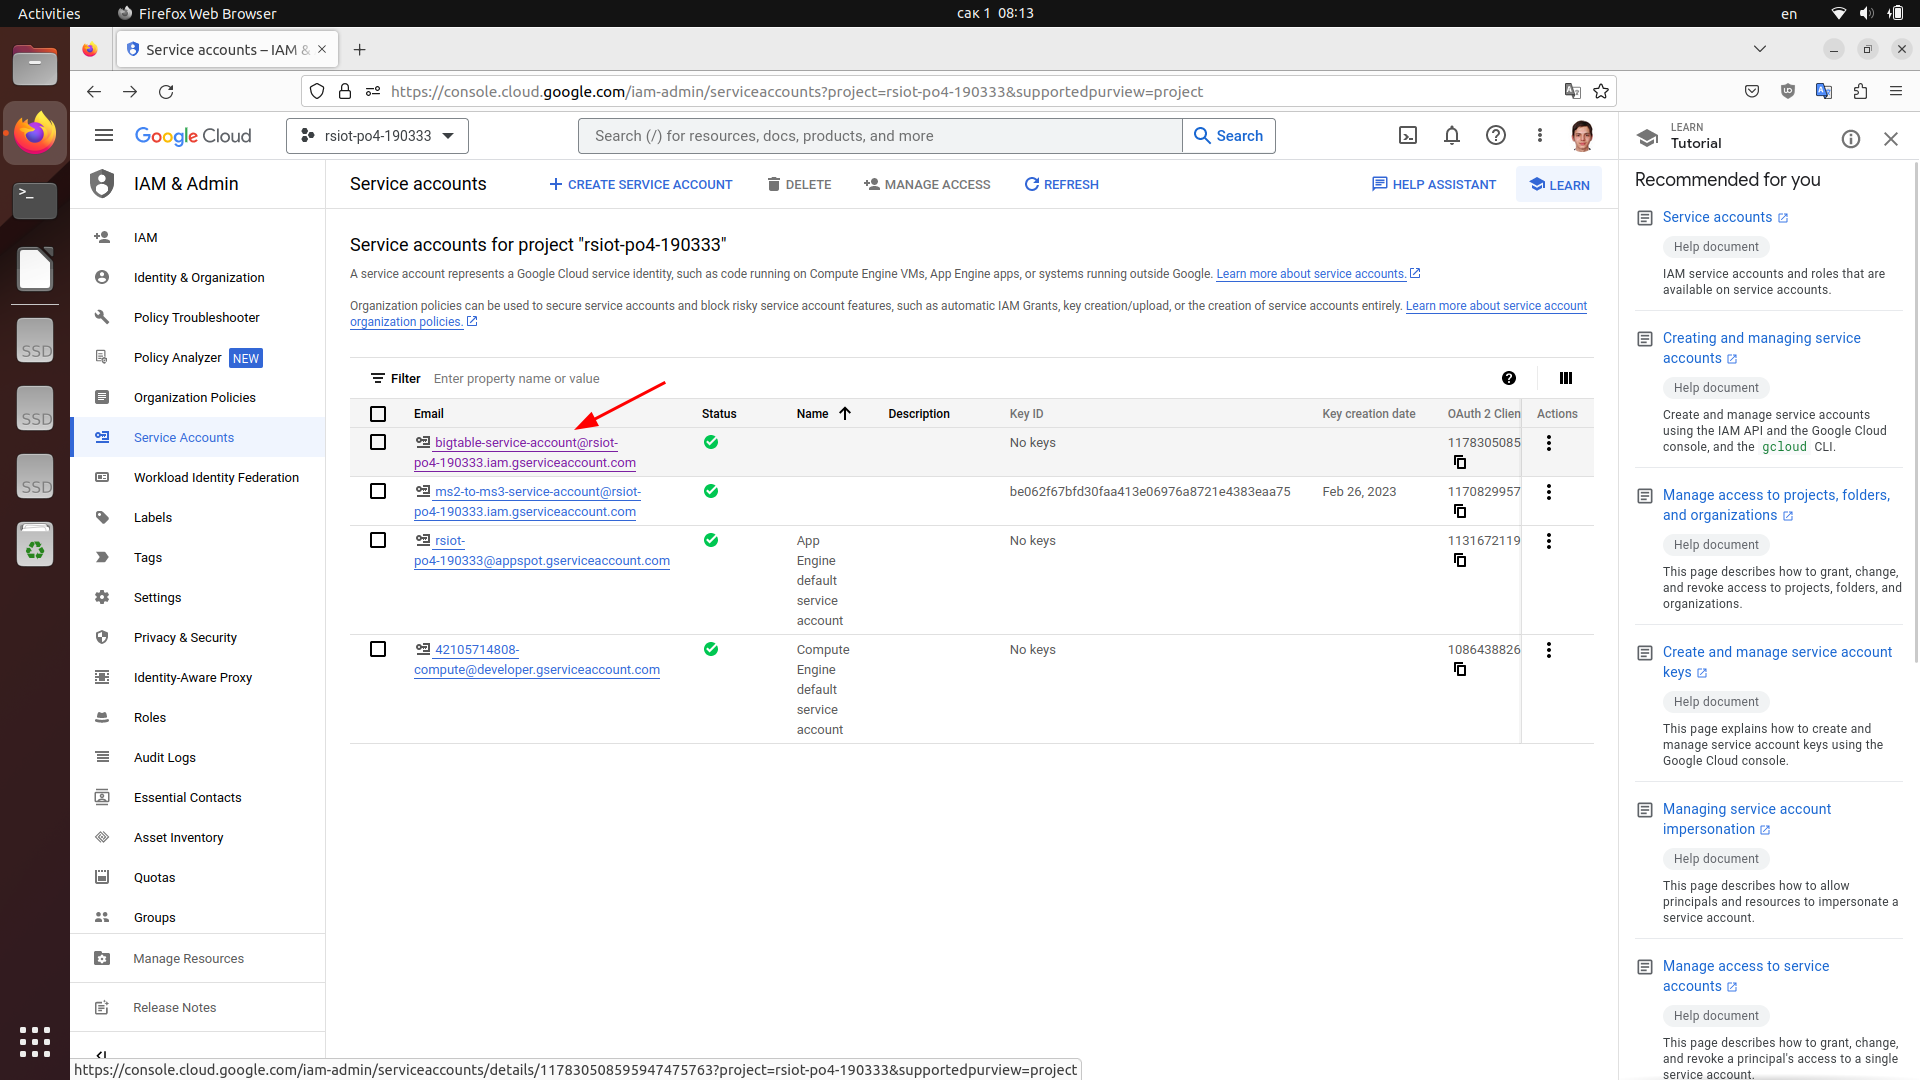
\includegraphics[width=10cm]
    {images/GoogleCloudBigTable/2023-03-01_08-13-26.png}
    \caption{\_}
    \label{fig:14}
  \end{figure}

  Жму KEYS > ADD KEY > Create new key (см. рисунок~\ref{fig:15}).

  \begin{figure}[!h]
    \centering
    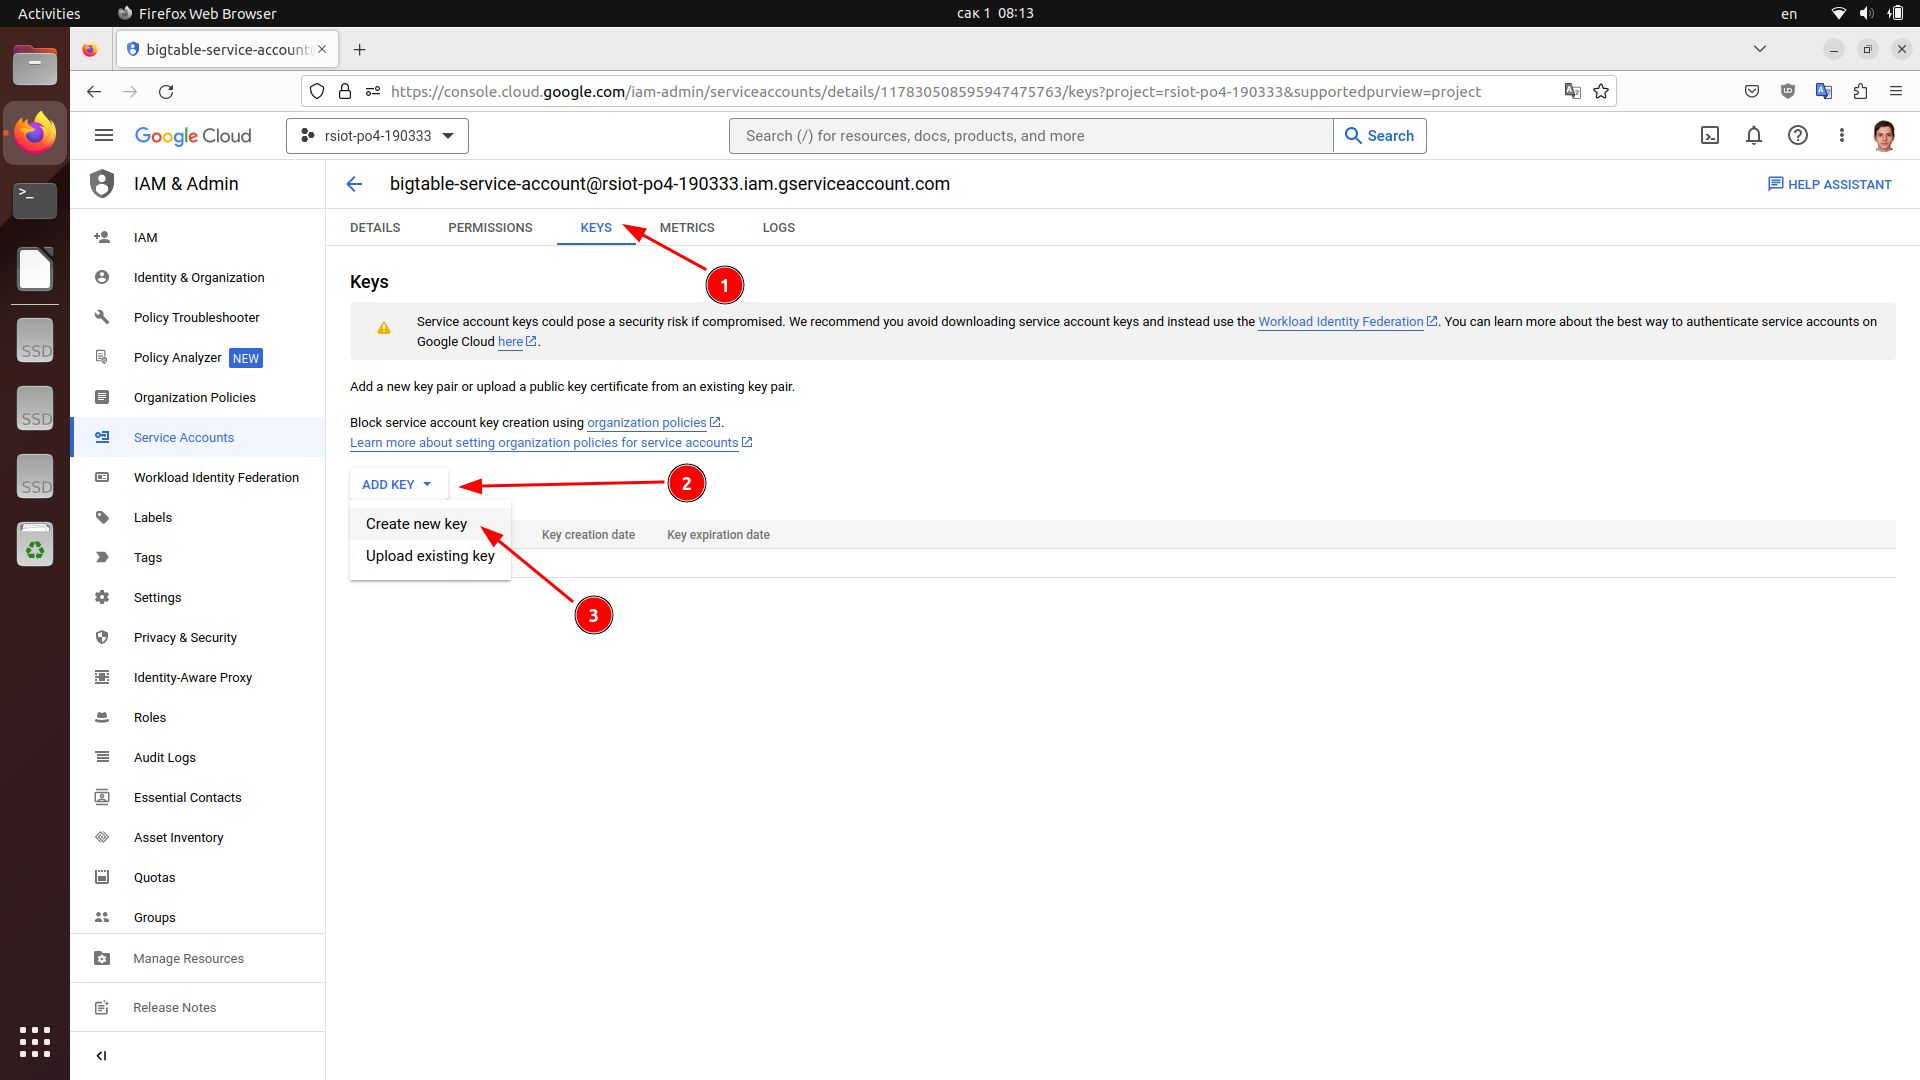
\includegraphics[width=10cm]
    {images/GoogleCloudBigTable/2023-03-01_08-14-23.png}
    \caption{\_}
    \label{fig:15}
  \end{figure}

  Жму JSON > CREATE (см. рисунок~\ref{fig:16}).

  \begin{figure}[!h]
    \centering
    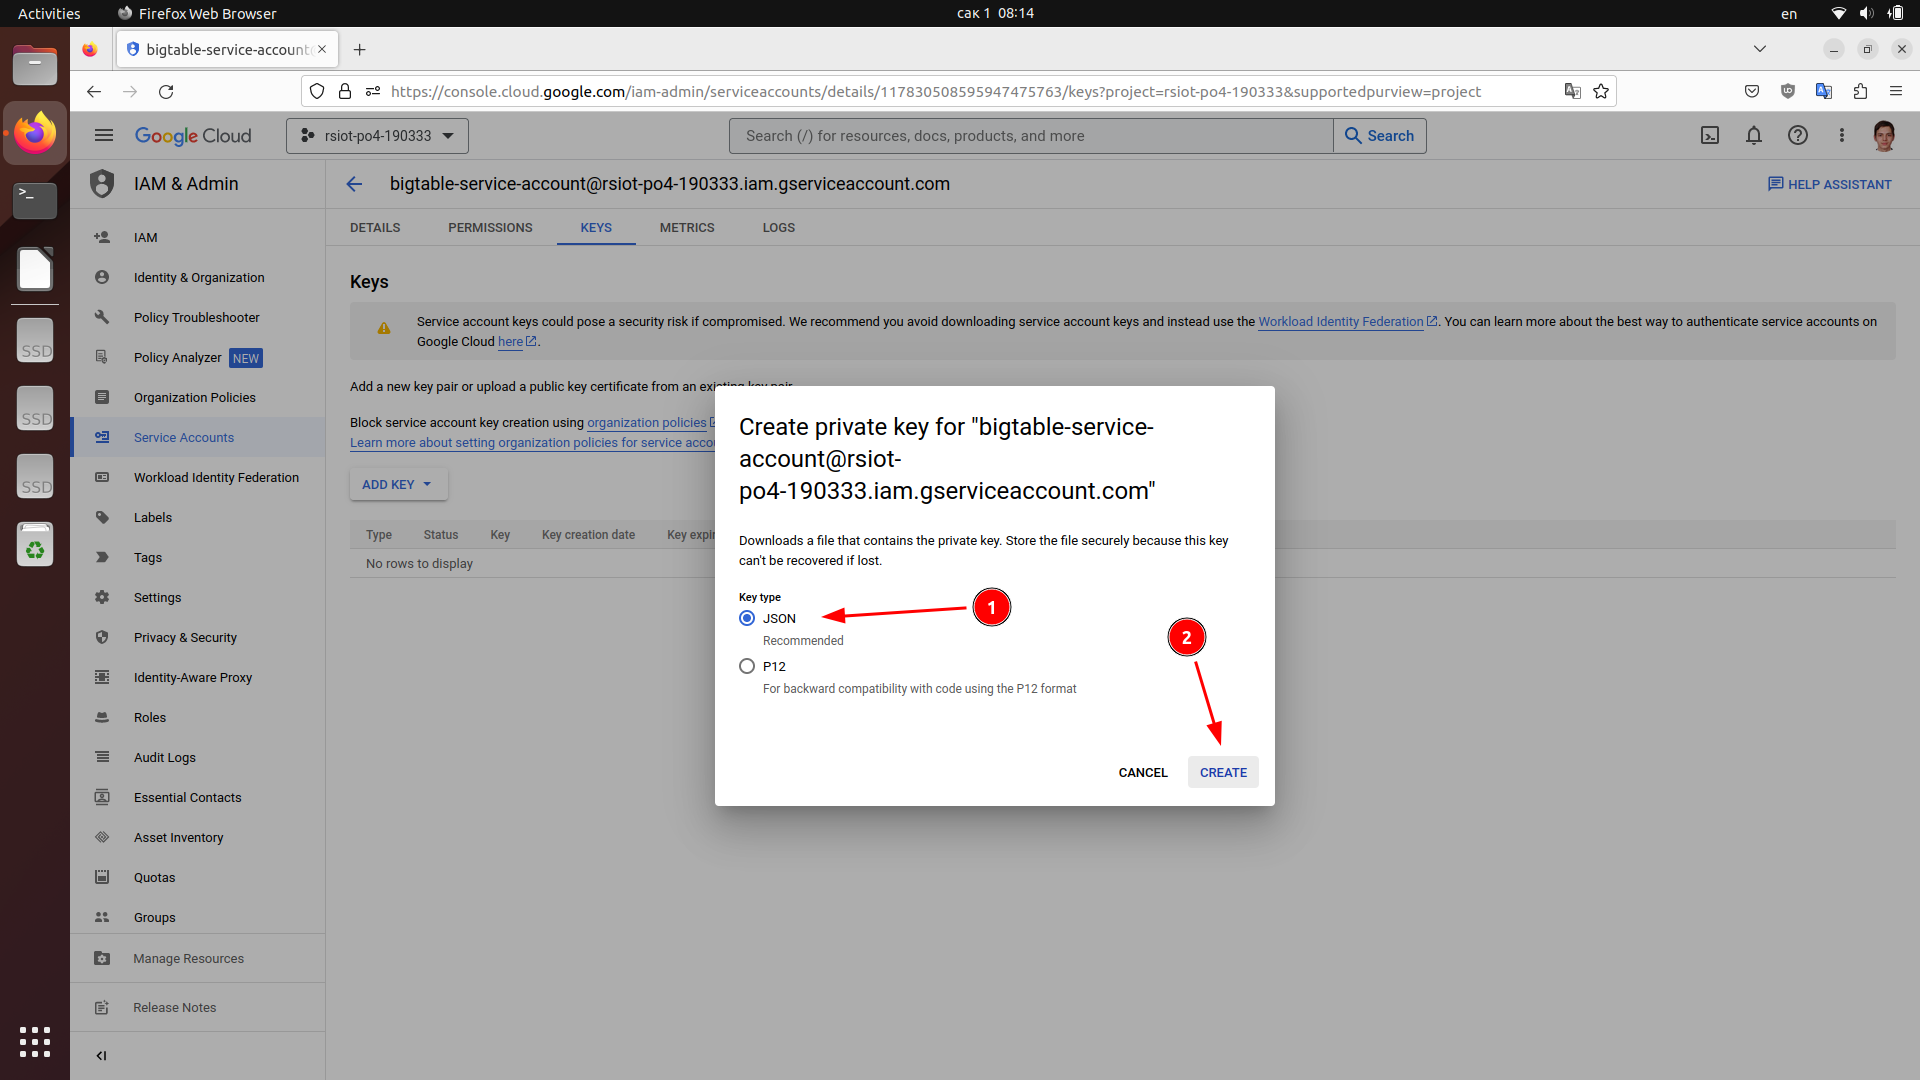
\includegraphics[width=10cm]
    {images/GoogleCloudBigTable/2023-03-01_08-14-41.png}
    \caption{\_}
    \label{fig:16}
  \end{figure}

  \newpage
  \begin{center}
    \textbf{Создание сервисного аккаунта для Google Cloud BigQuery}
  \end{center}

  Заходим на сайт Google Cloud Console \cite{GoogleCloudConsole} (см. рисунок~\ref{fig:17}).

  Menu > IAM \& Admin > Service Accounts \cite{GoogleCloudServiceAccounts} (см. рисунок~\ref{fig:17}).

  \begin{figure}[!h]
    \centering
    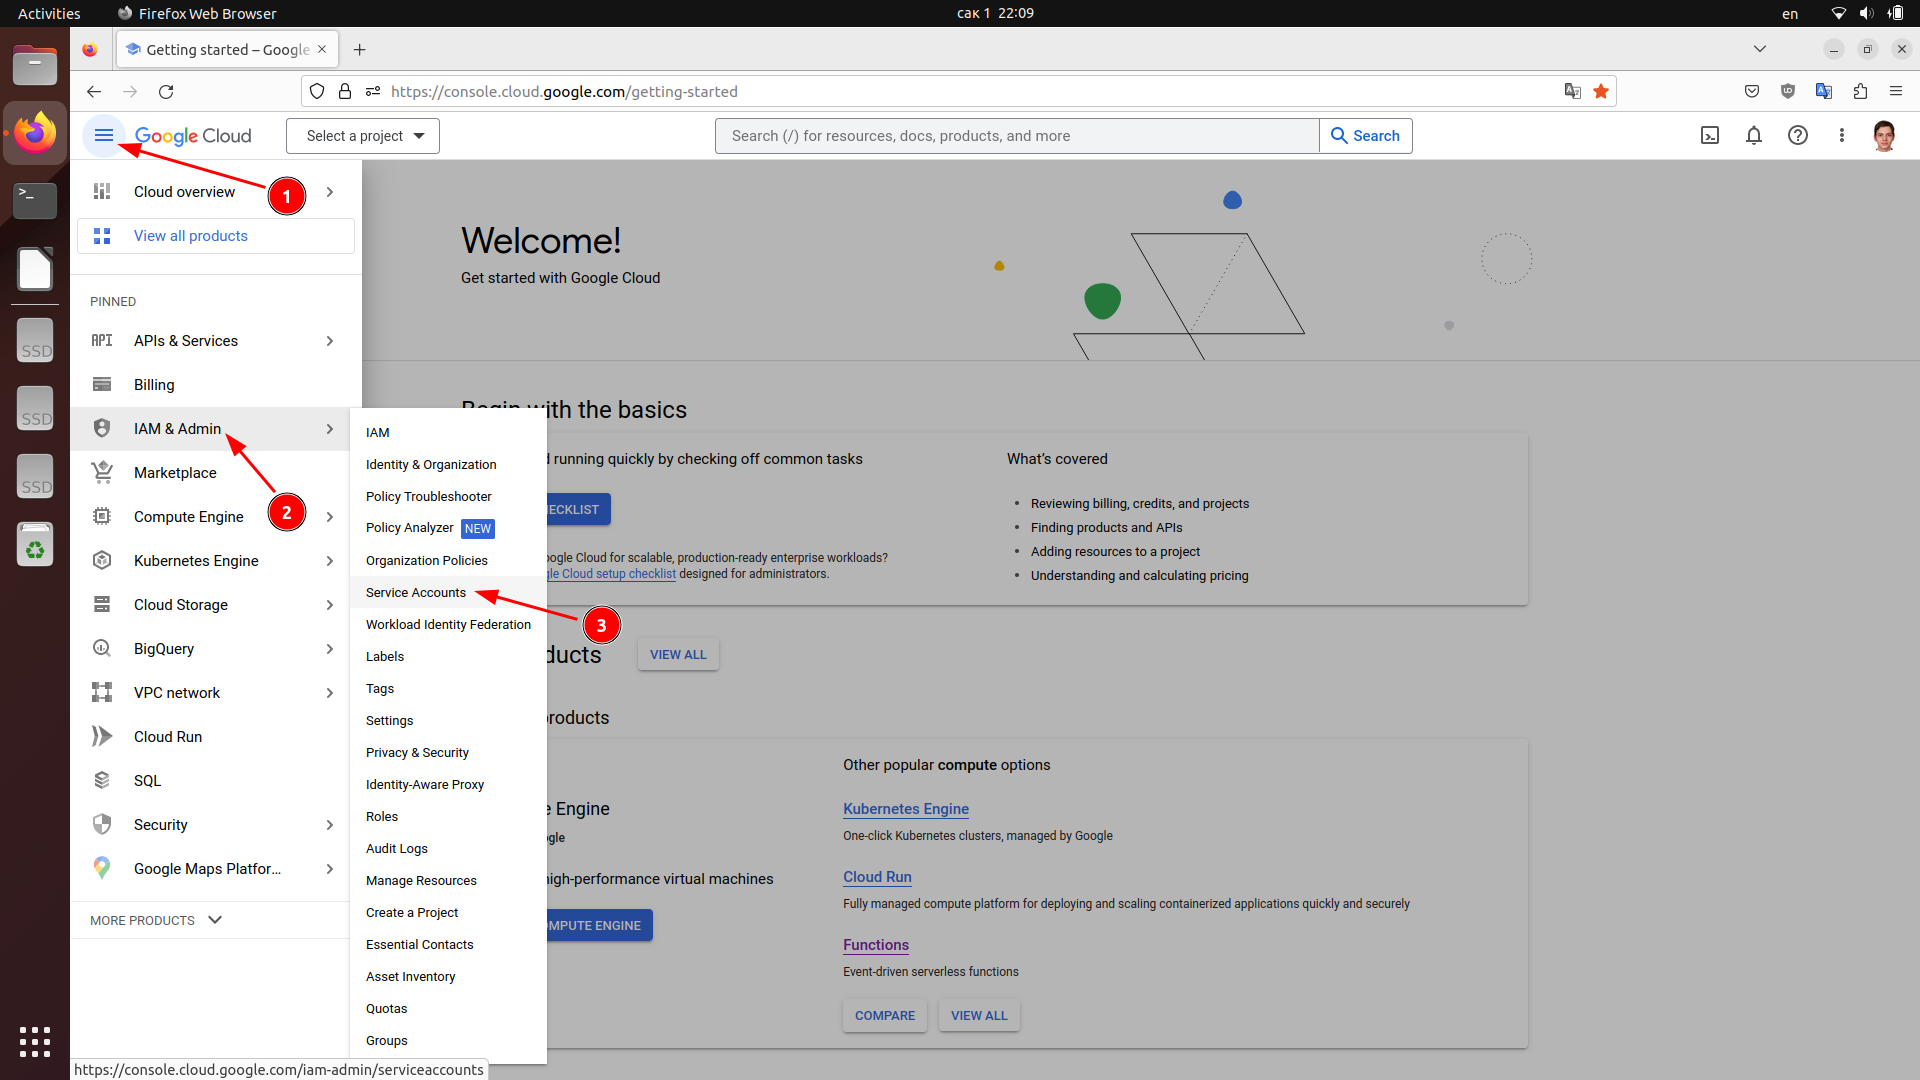
\includegraphics[width=10cm]
    {images/GoogleCloudBigQuery/2023-03-01_22-10-20.png}
    \caption{\_}
    \label{fig:17}
  \end{figure}

  Жму <<CREATE SERVICE ACCOUNT>> (см. рисунок~\ref{fig:18}).

  \begin{figure}[!h]
    \centering
    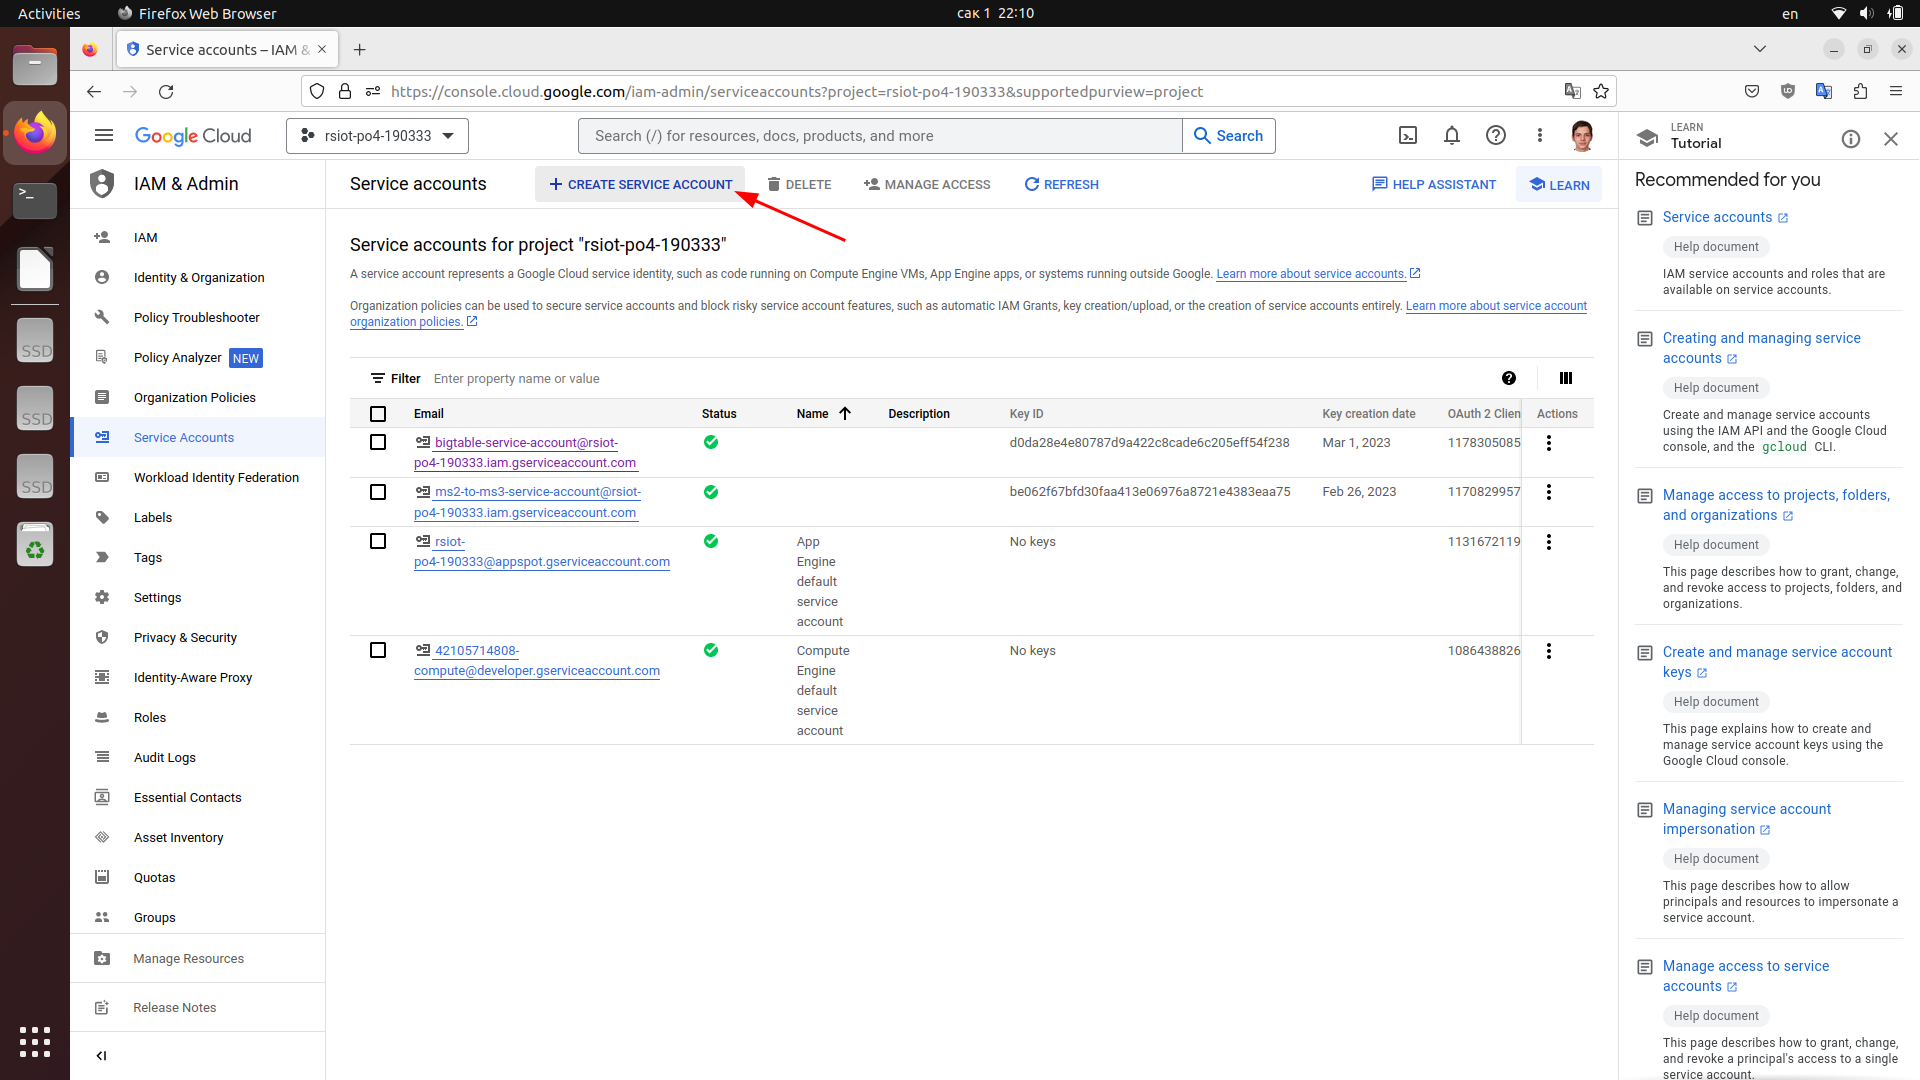
\includegraphics[width=10cm]
    {images/GoogleCloudBigQuery/2023-03-01_22-10-50.png}
    \caption{\_}
    \label{fig:18}
  \end{figure}

  Service account ID: \underline{bigquery-service-account} (см. рисунок~\ref{fig:19}).

  Жму <<CREATE SERVICE ACCOUNT>> (см. рисунок~\ref{fig:19}).

  \begin{figure}[!h]
    \centering
    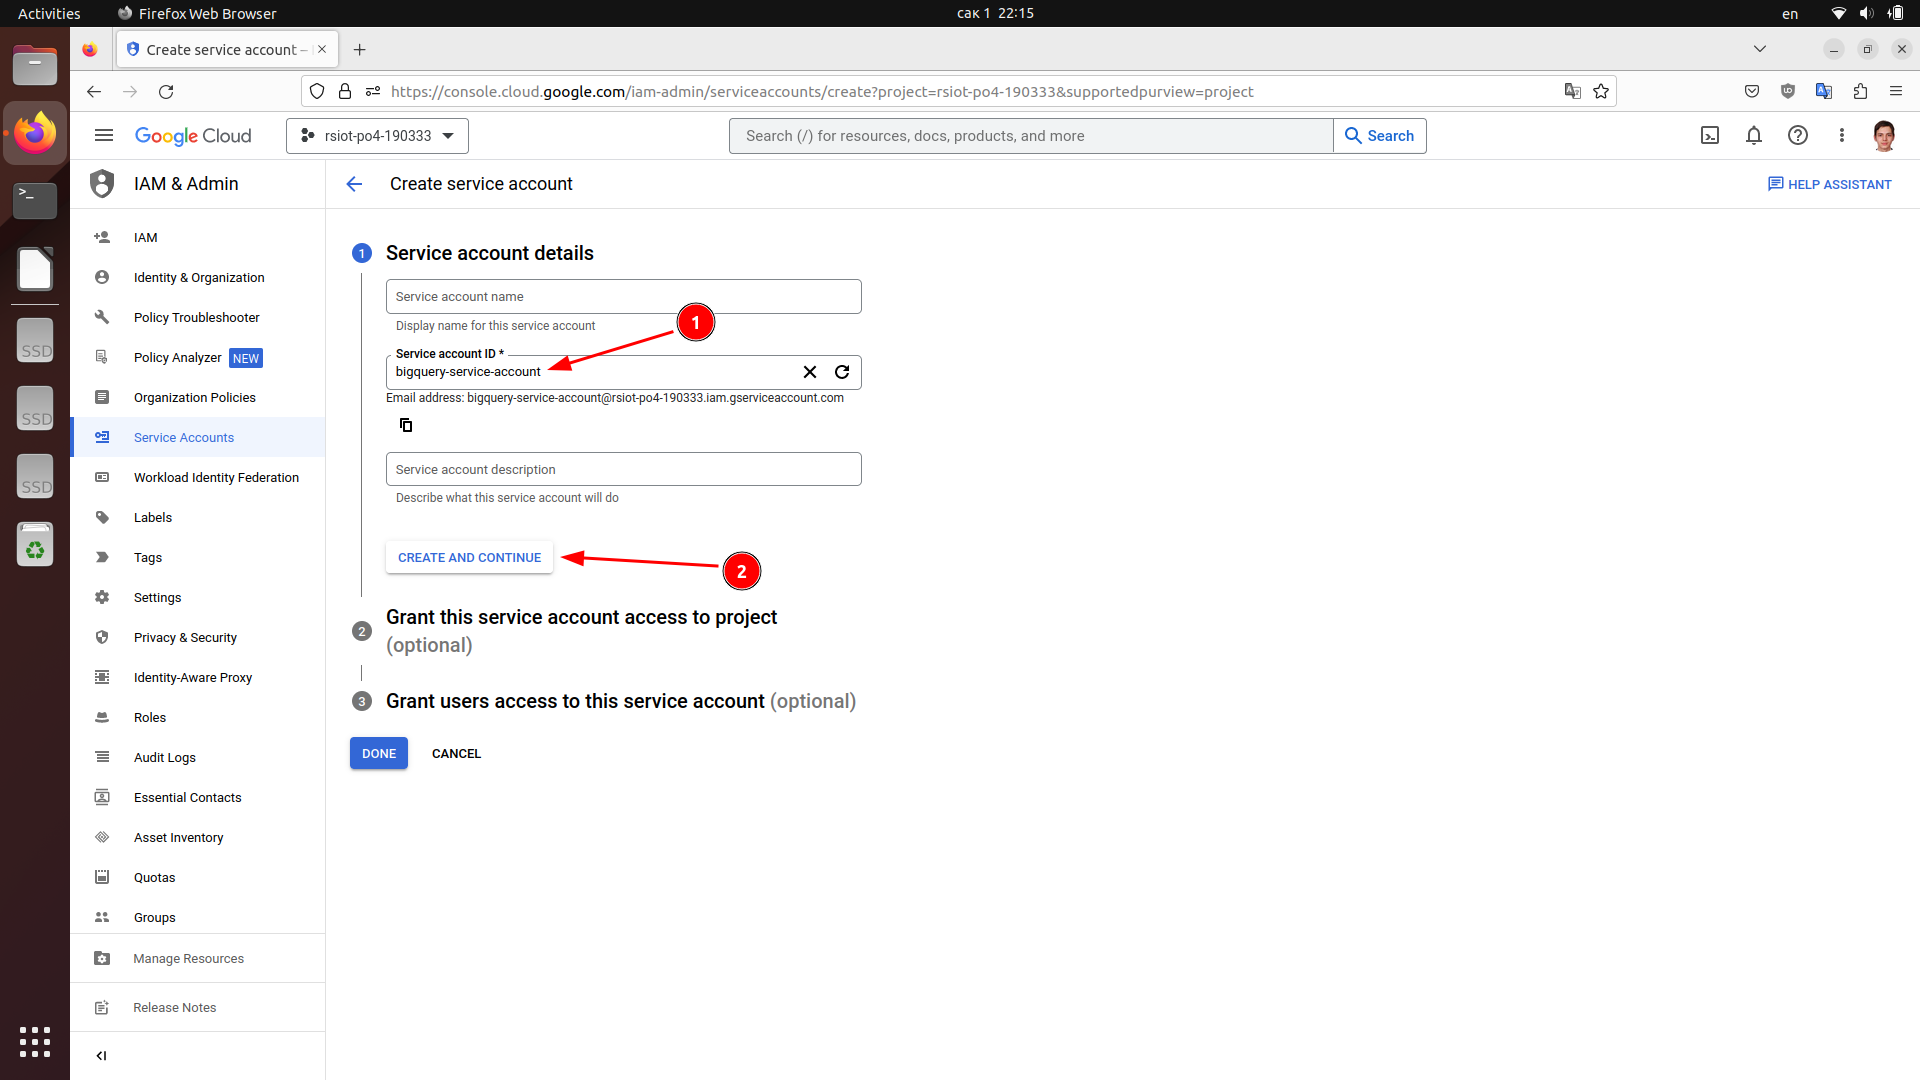
\includegraphics[width=10cm]
    {images/GoogleCloudBigQuery/2023-03-01_22-15-46.png}
    \caption{\_}
    \label{fig:19}
  \end{figure}

  Жму Select a role > Cloud Bigtable > Bigtable Administrator (см. рисунок~\ref{fig:20}).

  Жму <<CONTINUE>> (см. рисунок~\ref{fig:20}).

  \begin{figure}[!h]
    \centering
    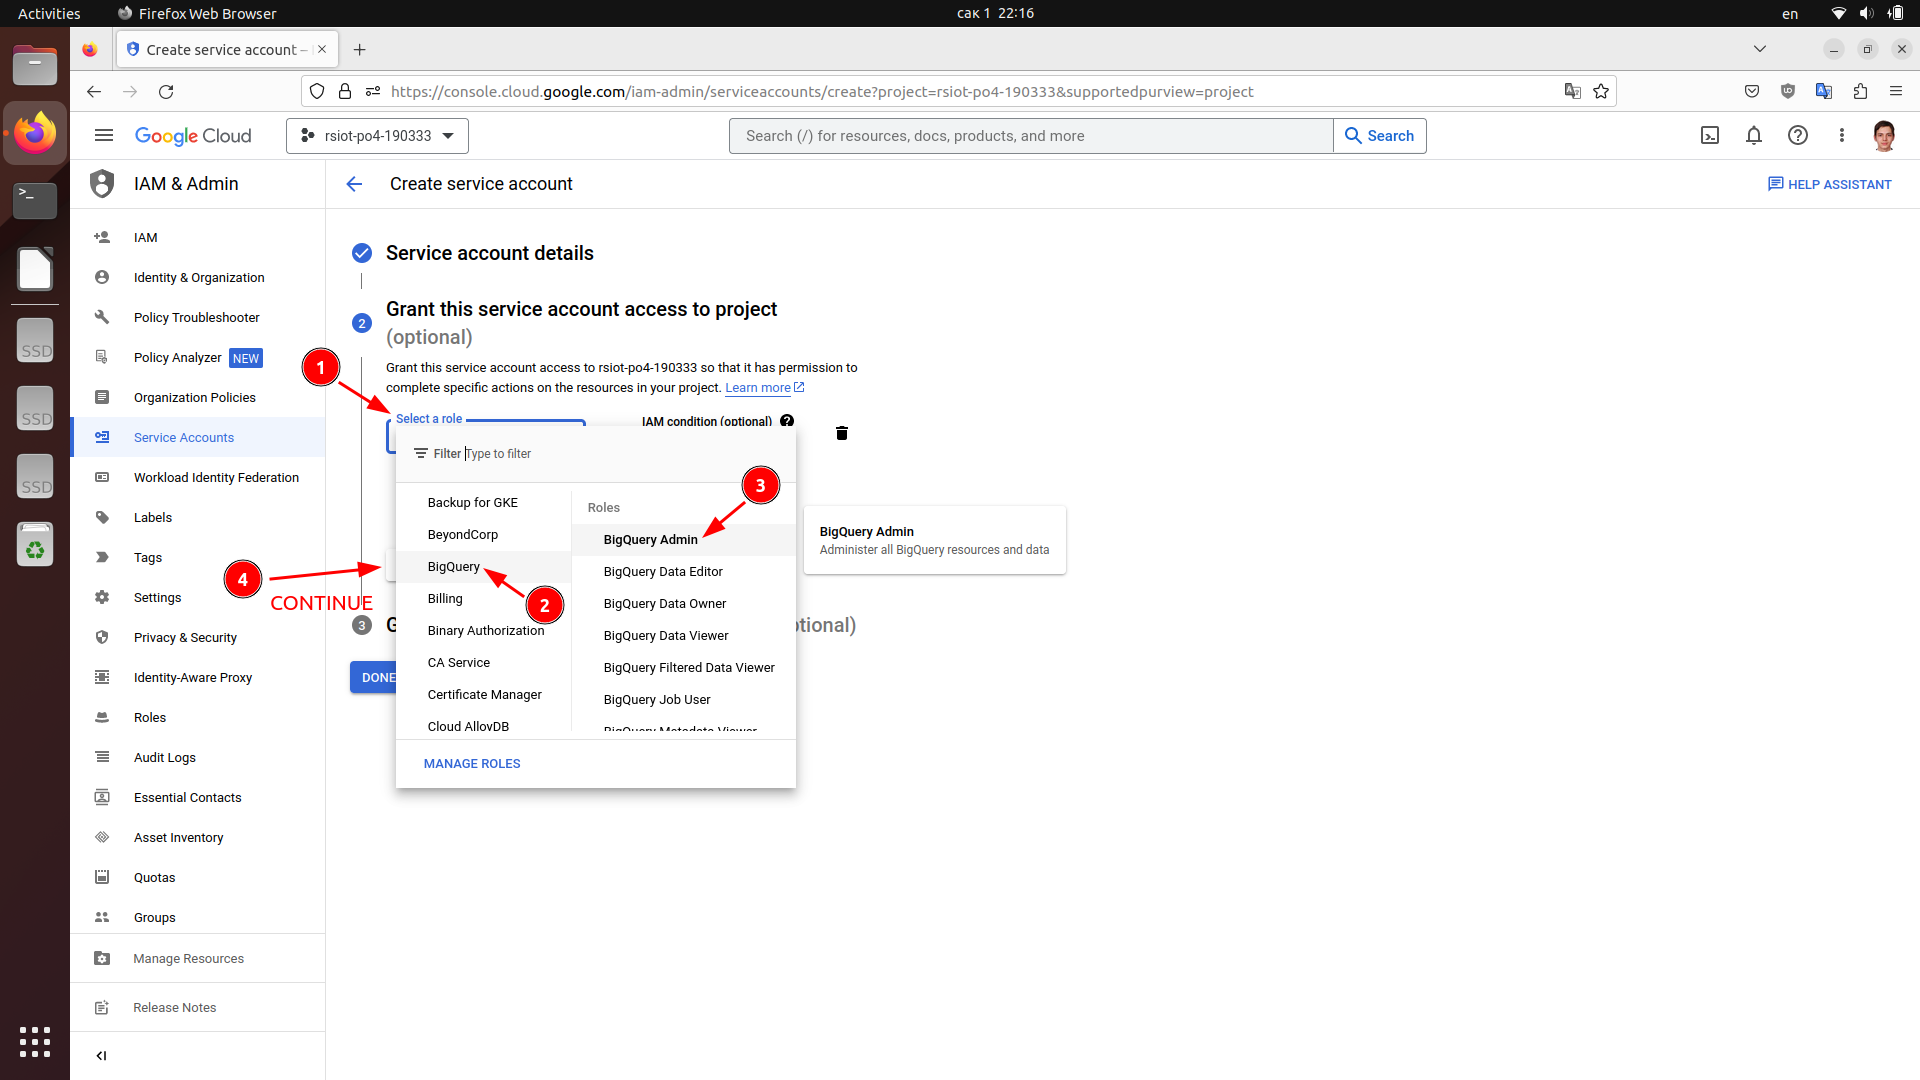
\includegraphics[width=18cm]
    {images/GoogleCloudBigQuery/2023-03-01_22-17-10.png}
    \caption{\_}
    \label{fig:20}
  \end{figure}

  Жму <<DONE>> (см. рисунок~\ref{fig:21}).

  \begin{figure}[!h]
    \centering
    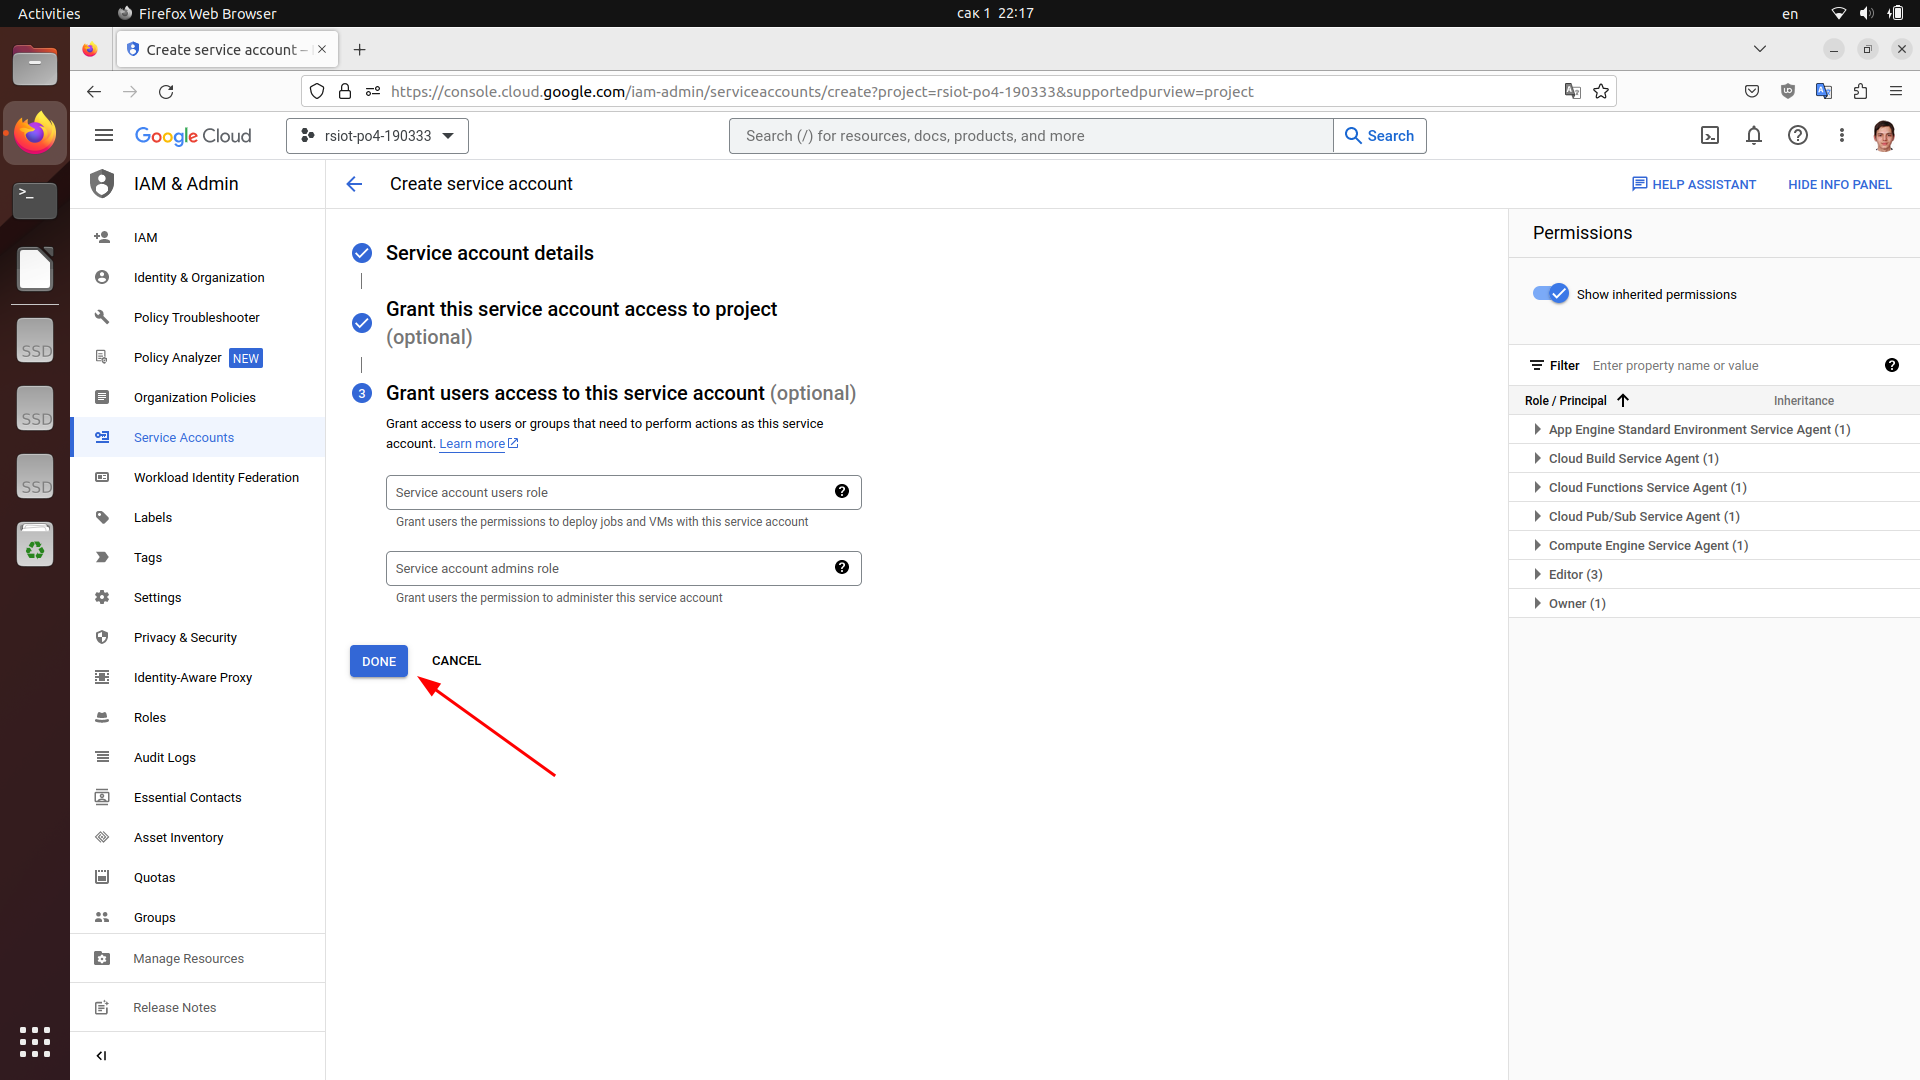
\includegraphics[width=18cm]
    {images/GoogleCloudBigQuery/2023-03-01_22-17-30.png}
    \caption{\_}
    \label{fig:21}
  \end{figure}

  \newpage
  \begin{center}
    \textbf{Создание приватного ключа для Google Cloud BigQuery}
  \end{center}

  Жму по почту сервисного аккаунта: \\
  \underline{bigtable-service-account@rsiot-po4-190333.iam.gserviceaccount.com} (см. рисунок~\ref{fig:22}).
  
  \begin{figure}[!h]
    \centering
    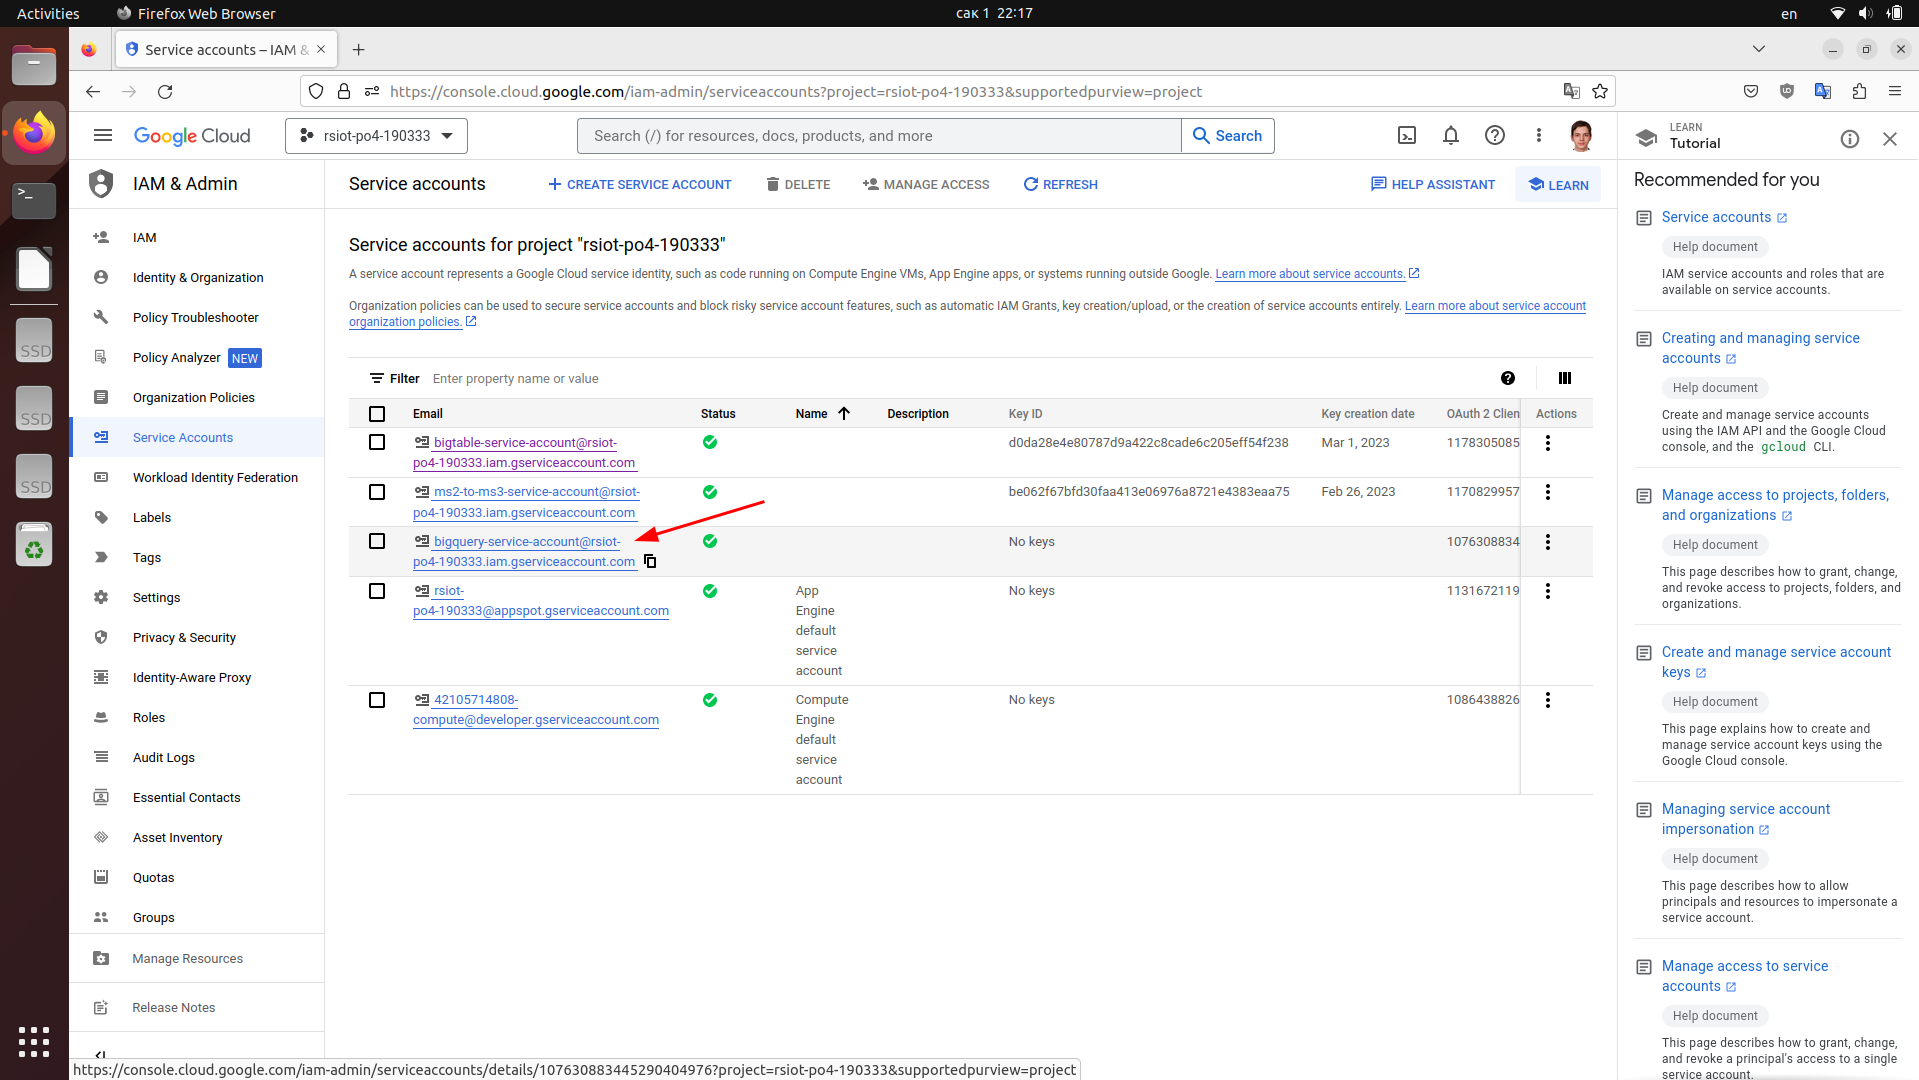
\includegraphics[width=10cm]
    {images/GoogleCloudBigQuery/2023-03-01_22-17-52.png}
    \caption{\_}
    \label{fig:22}
  \end{figure}

  Жму KEYS > ADD KEY > Create new key (см. рисунок~\ref{fig:23}).

  \begin{figure}[!h]
    \centering
    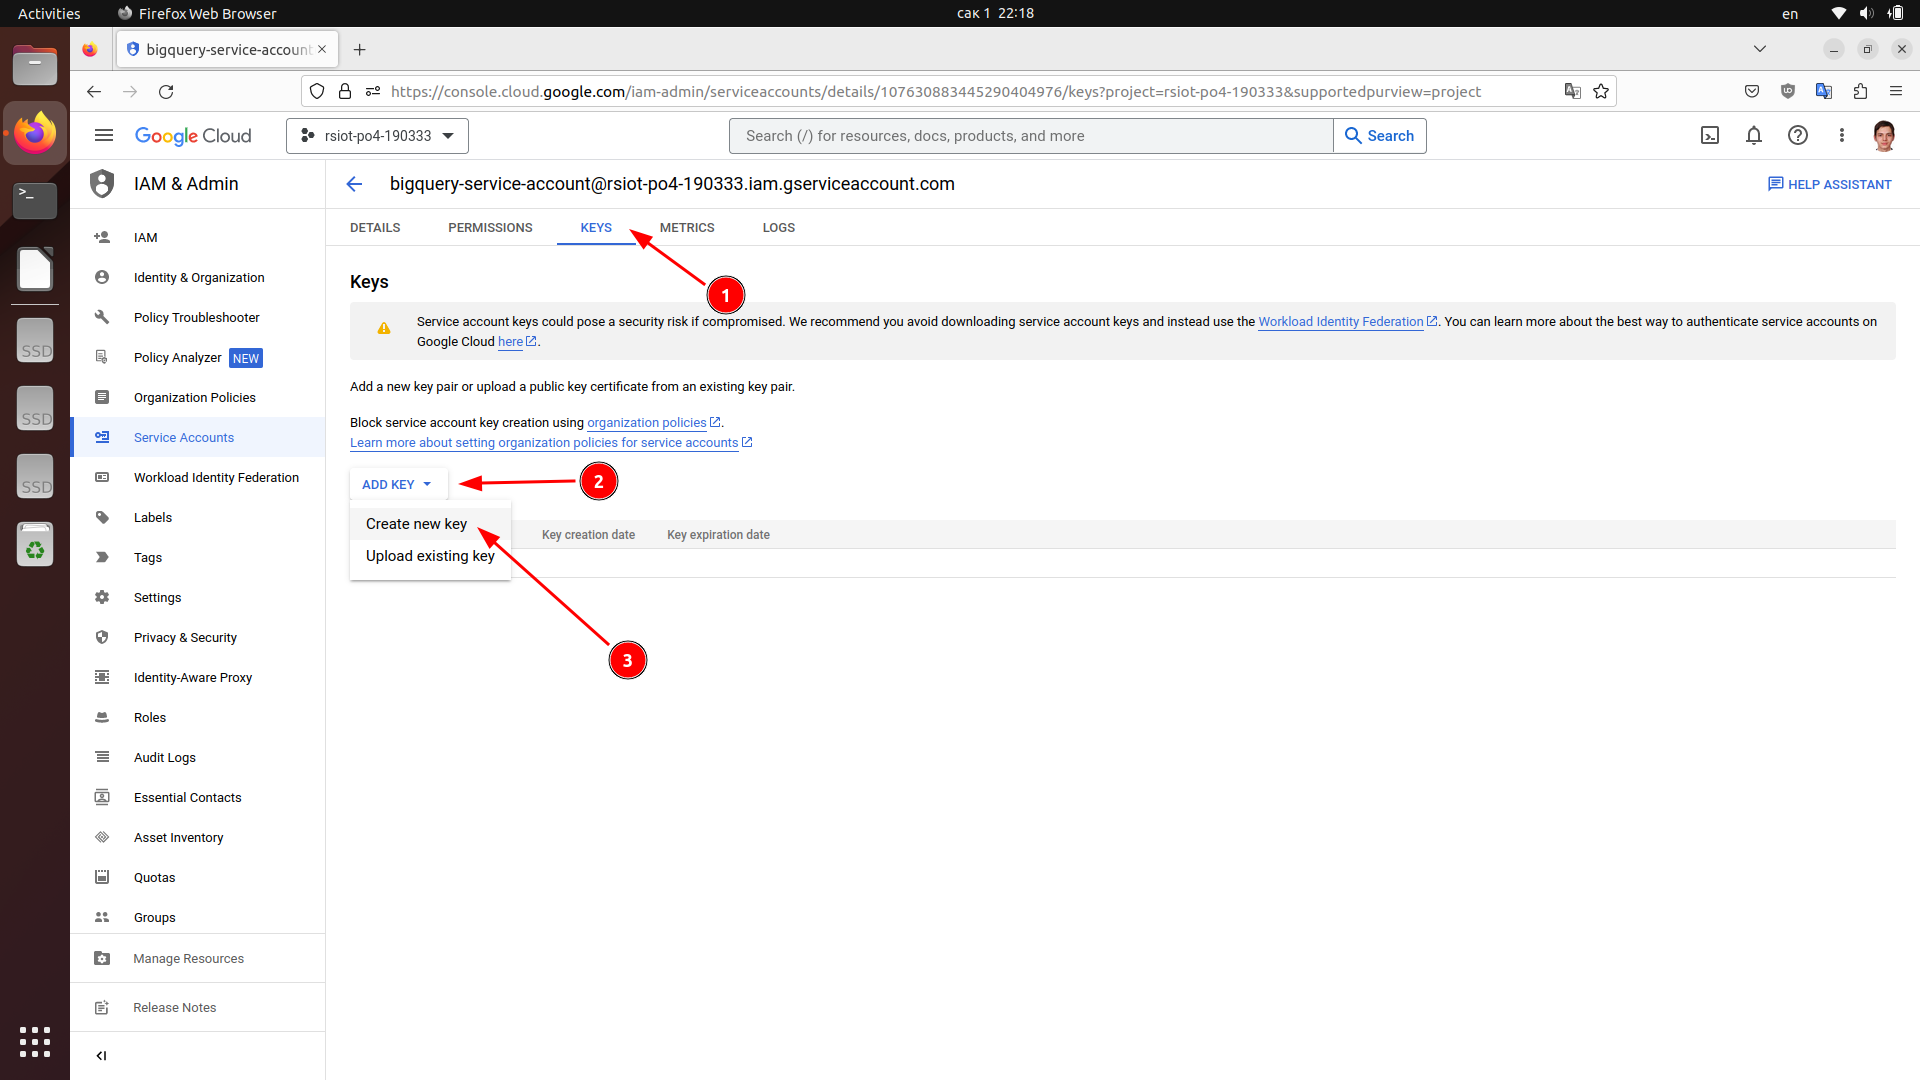
\includegraphics[width=10cm]
    {images/GoogleCloudBigQuery/2023-03-01_22-18-26.png}
    \caption{\_}
    \label{fig:23}
  \end{figure}

  Жму JSON > CREATE (см. рисунок~\ref{fig:24}).

  \begin{figure}[!h]
    \centering
    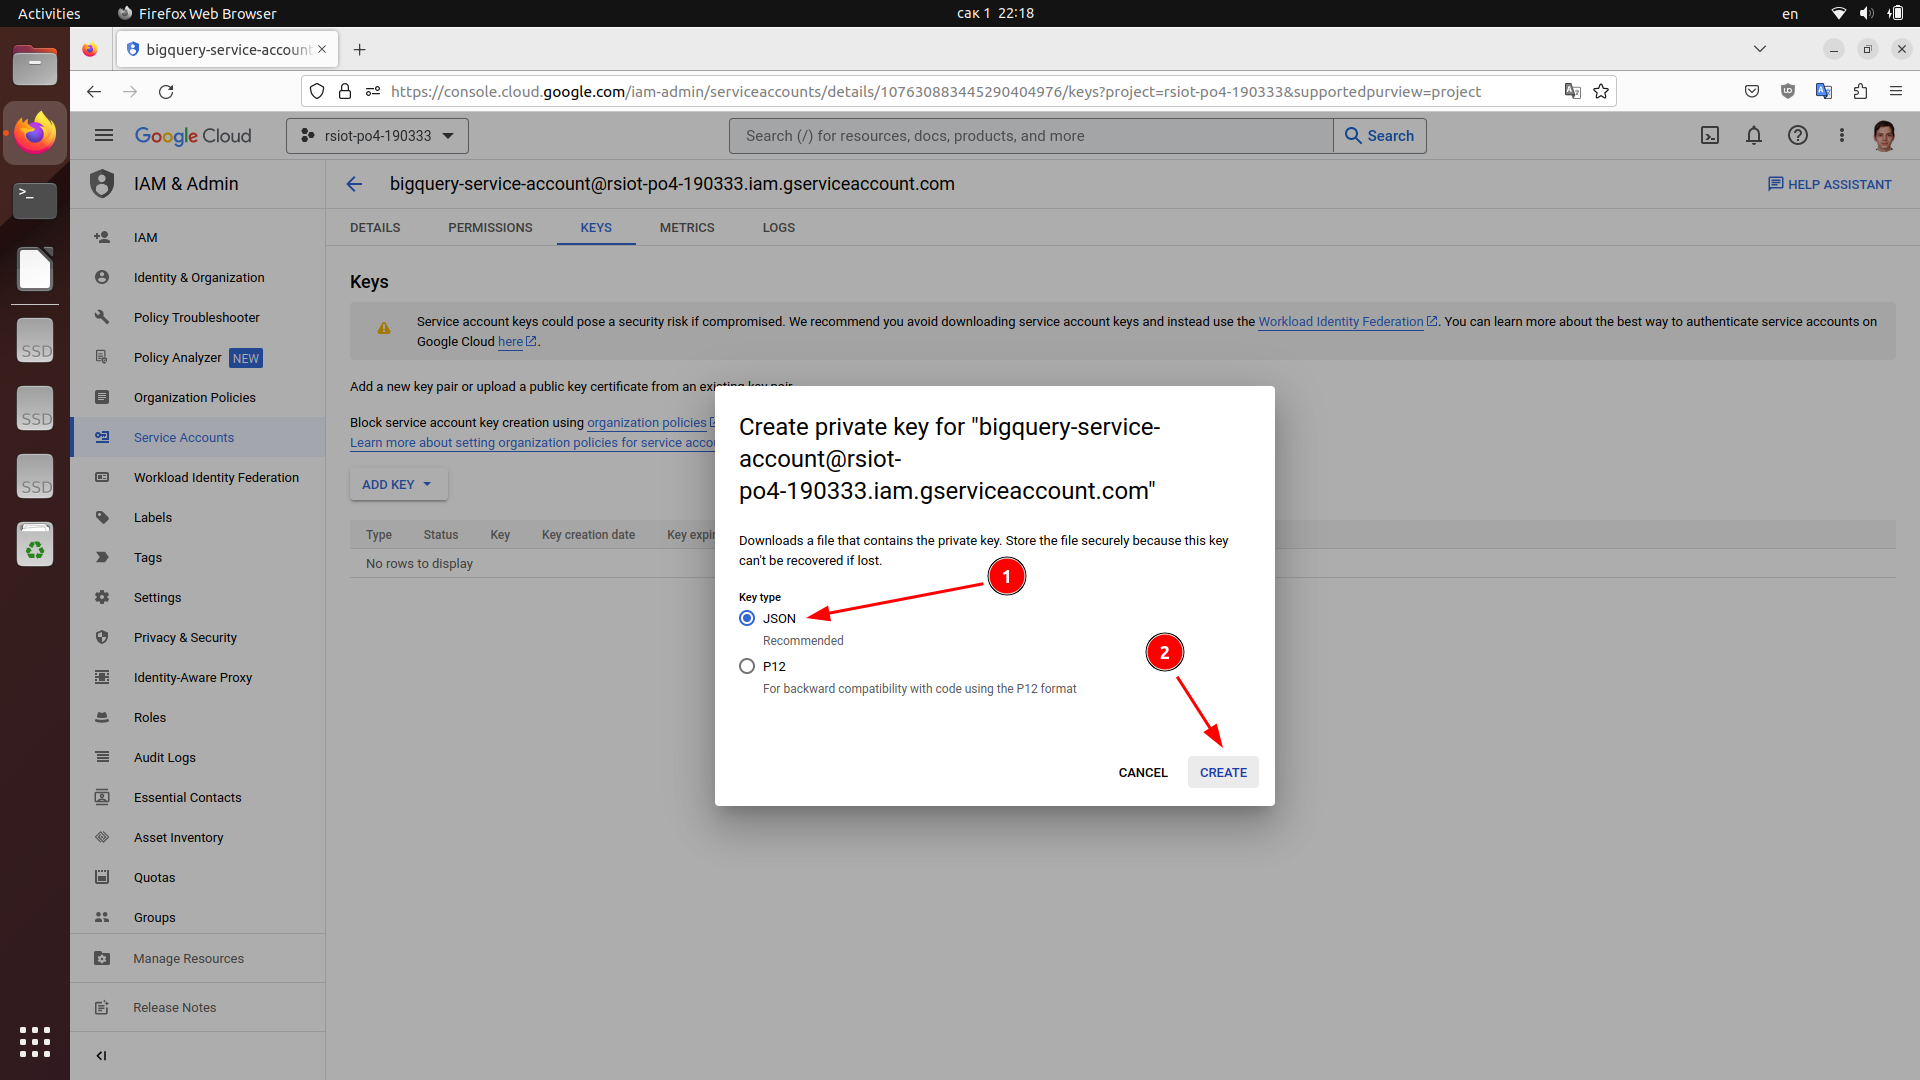
\includegraphics[width=10cm]
    {images/GoogleCloudBigQuery/2023-03-01_22-18-46.png}
    \caption{\_}
    \label{fig:24}
  \end{figure}

  \newpage
  \begin{center}
    \textbf{Создание MS4 в Google Cloud Functions}
  \end{center}

  Заходим на сайт Google Cloud Console \cite{GoogleCloudConsole} (см. рисунок~\ref{fig:25}).

  Menu > Cloud Functions \cite{GoogleCloudFunctions} (см. рисунок~\ref{fig:25}).

  \begin{figure}[!h]
    \centering
    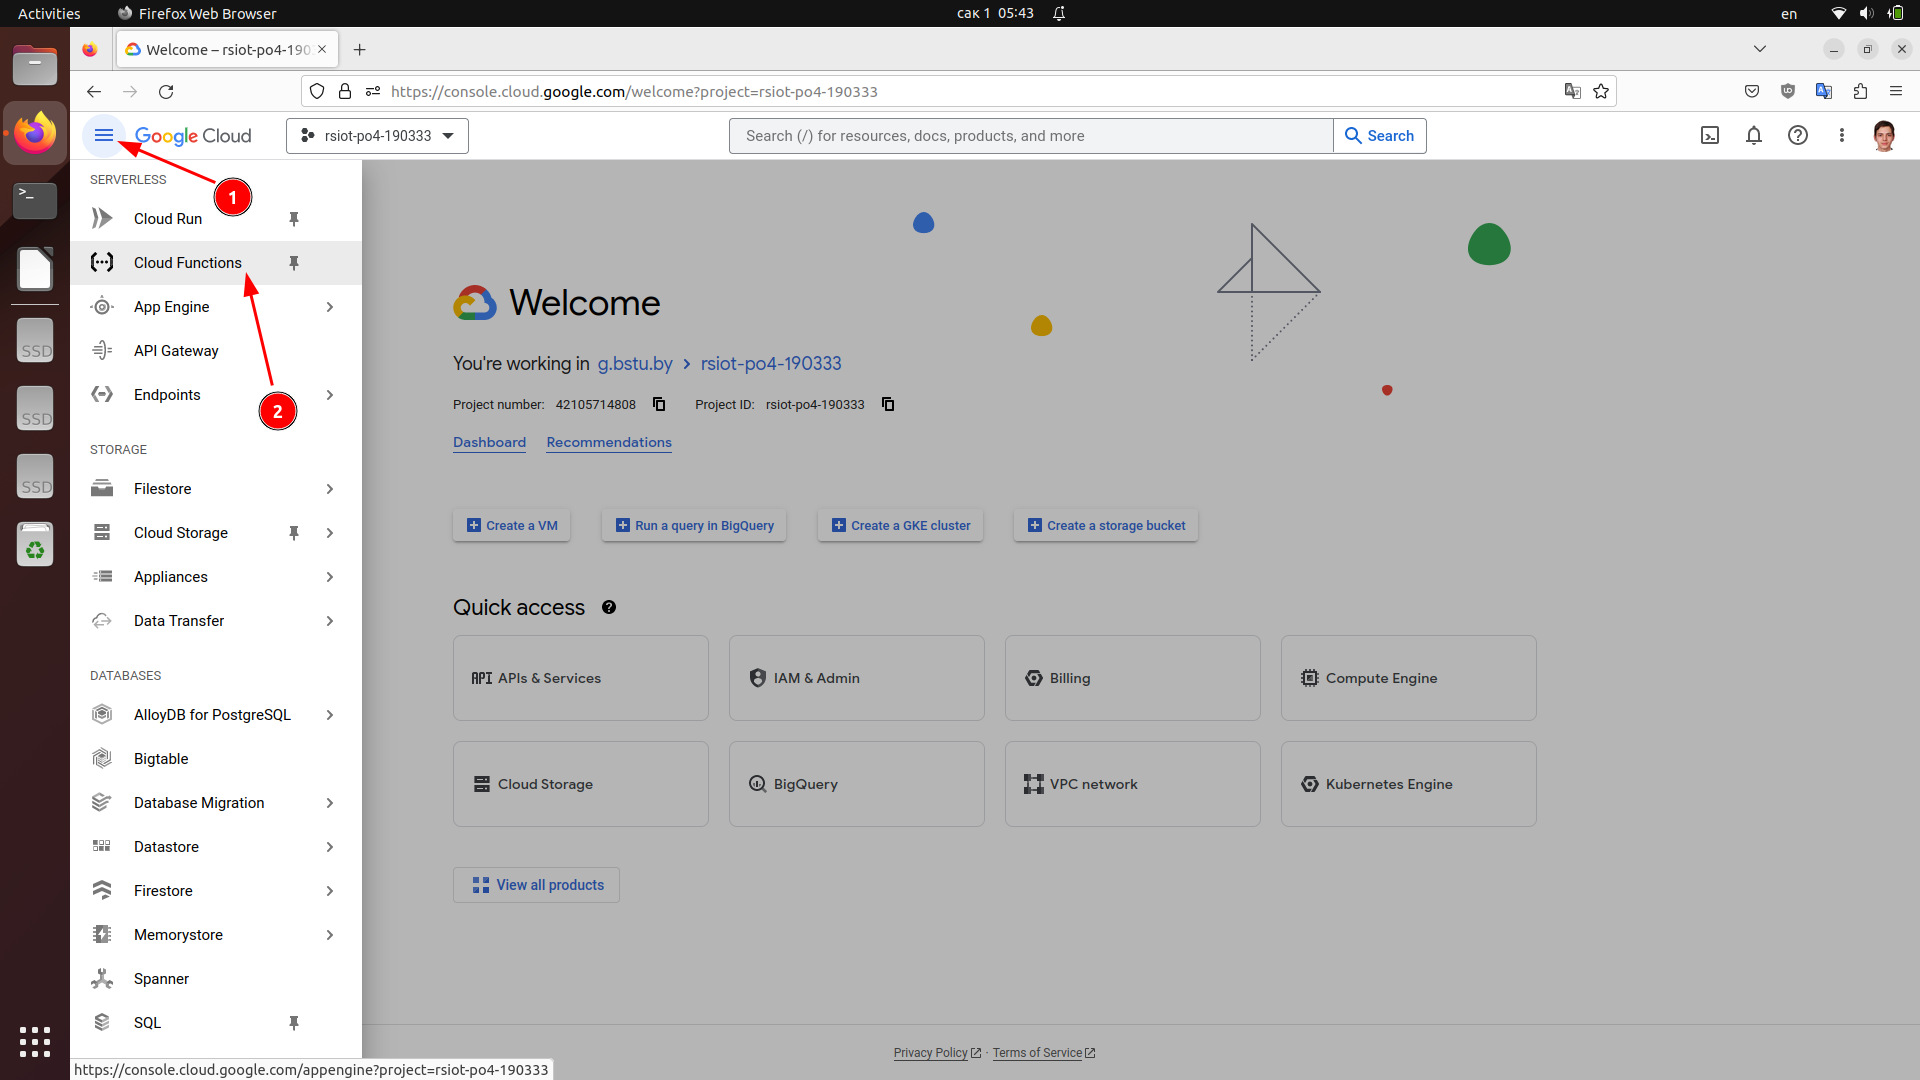
\includegraphics[width=10cm]
    {images/GoogleCloudFunctions/2023-03-01_05-43-48.png}
    \caption{\_}
    \label{fig:25}
  \end{figure}

  Жму <<CREATE FUNCTION>> (см. рисунок~\ref{fig:26}).

  \begin{figure}[!h]
    \centering
    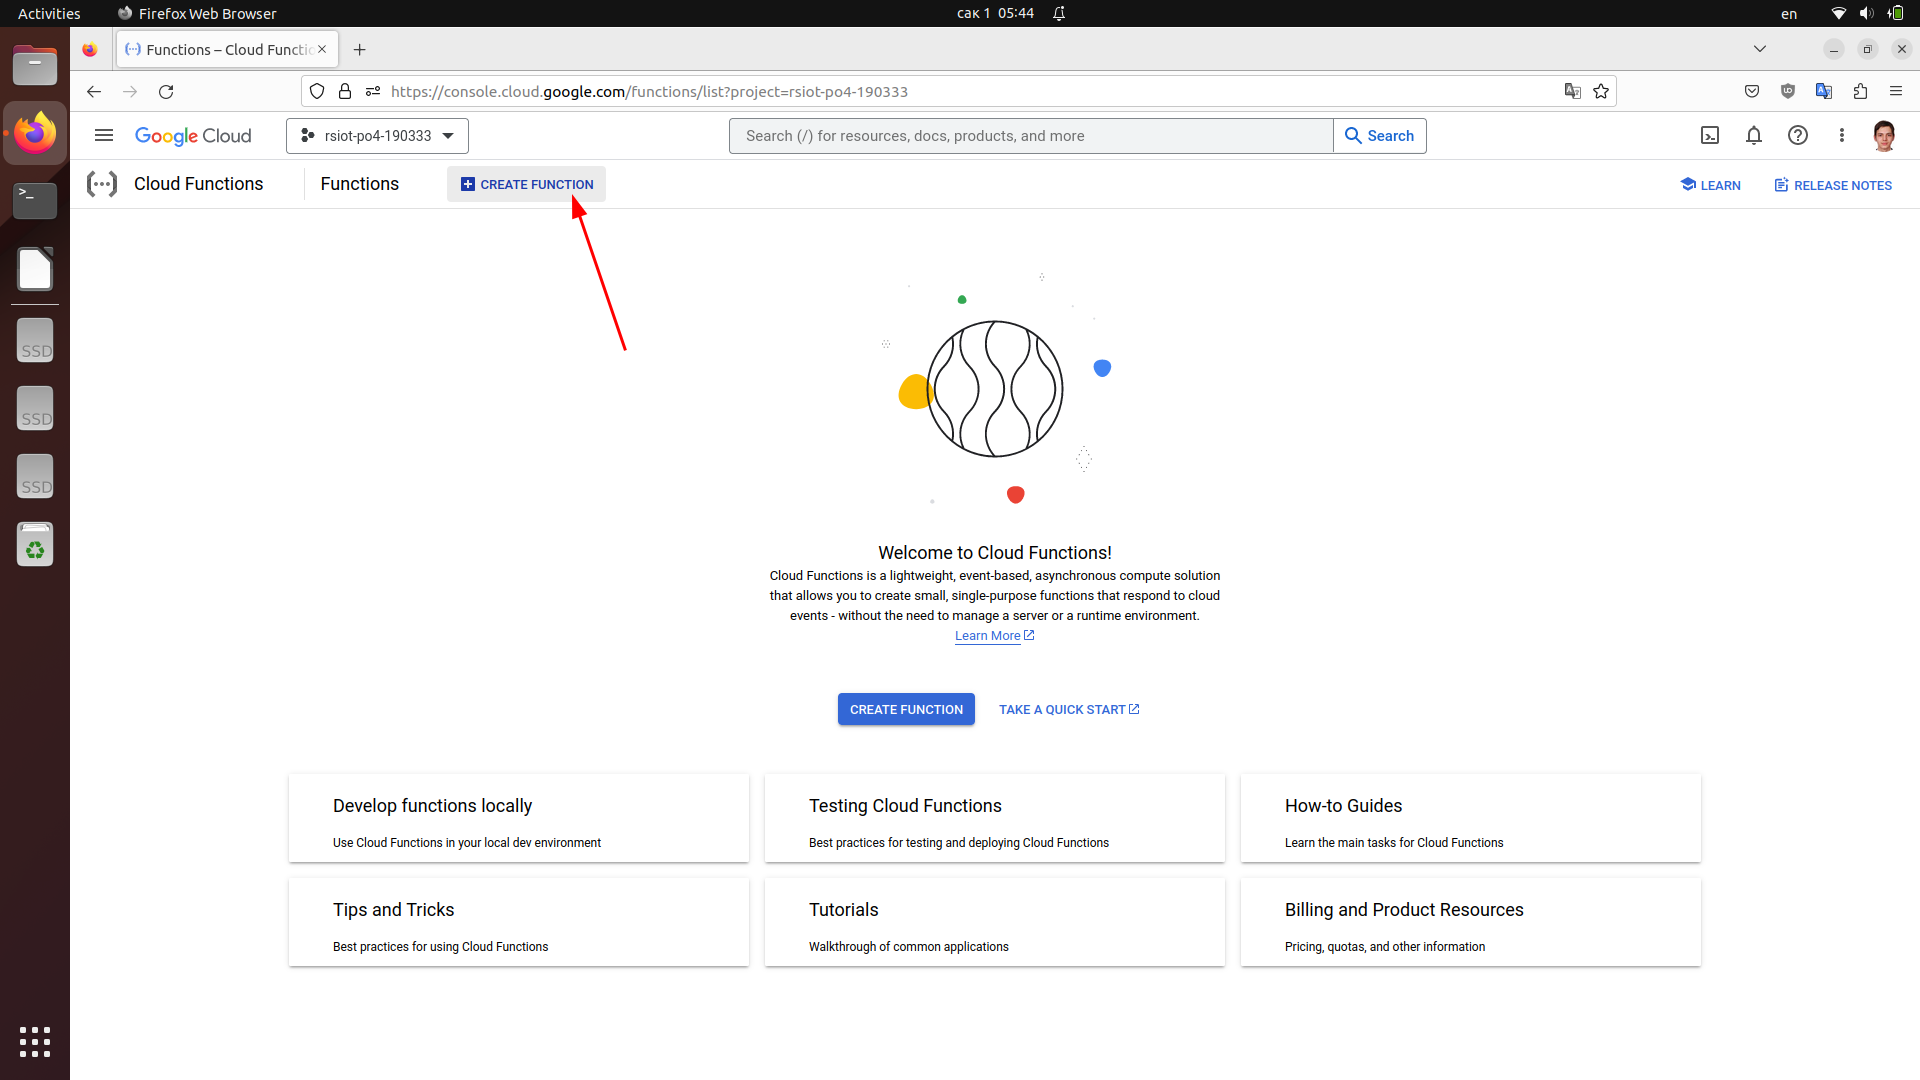
\includegraphics[width=10cm]
    {images/GoogleCloudFunctions/2023-03-01_05-44-11.png}
    \caption{\_}
    \label{fig:26}
  \end{figure}

  Включаем, если нужно, API (см. рисунок~\ref{fig:27}).

  \begin{figure}[!h]
    \centering
    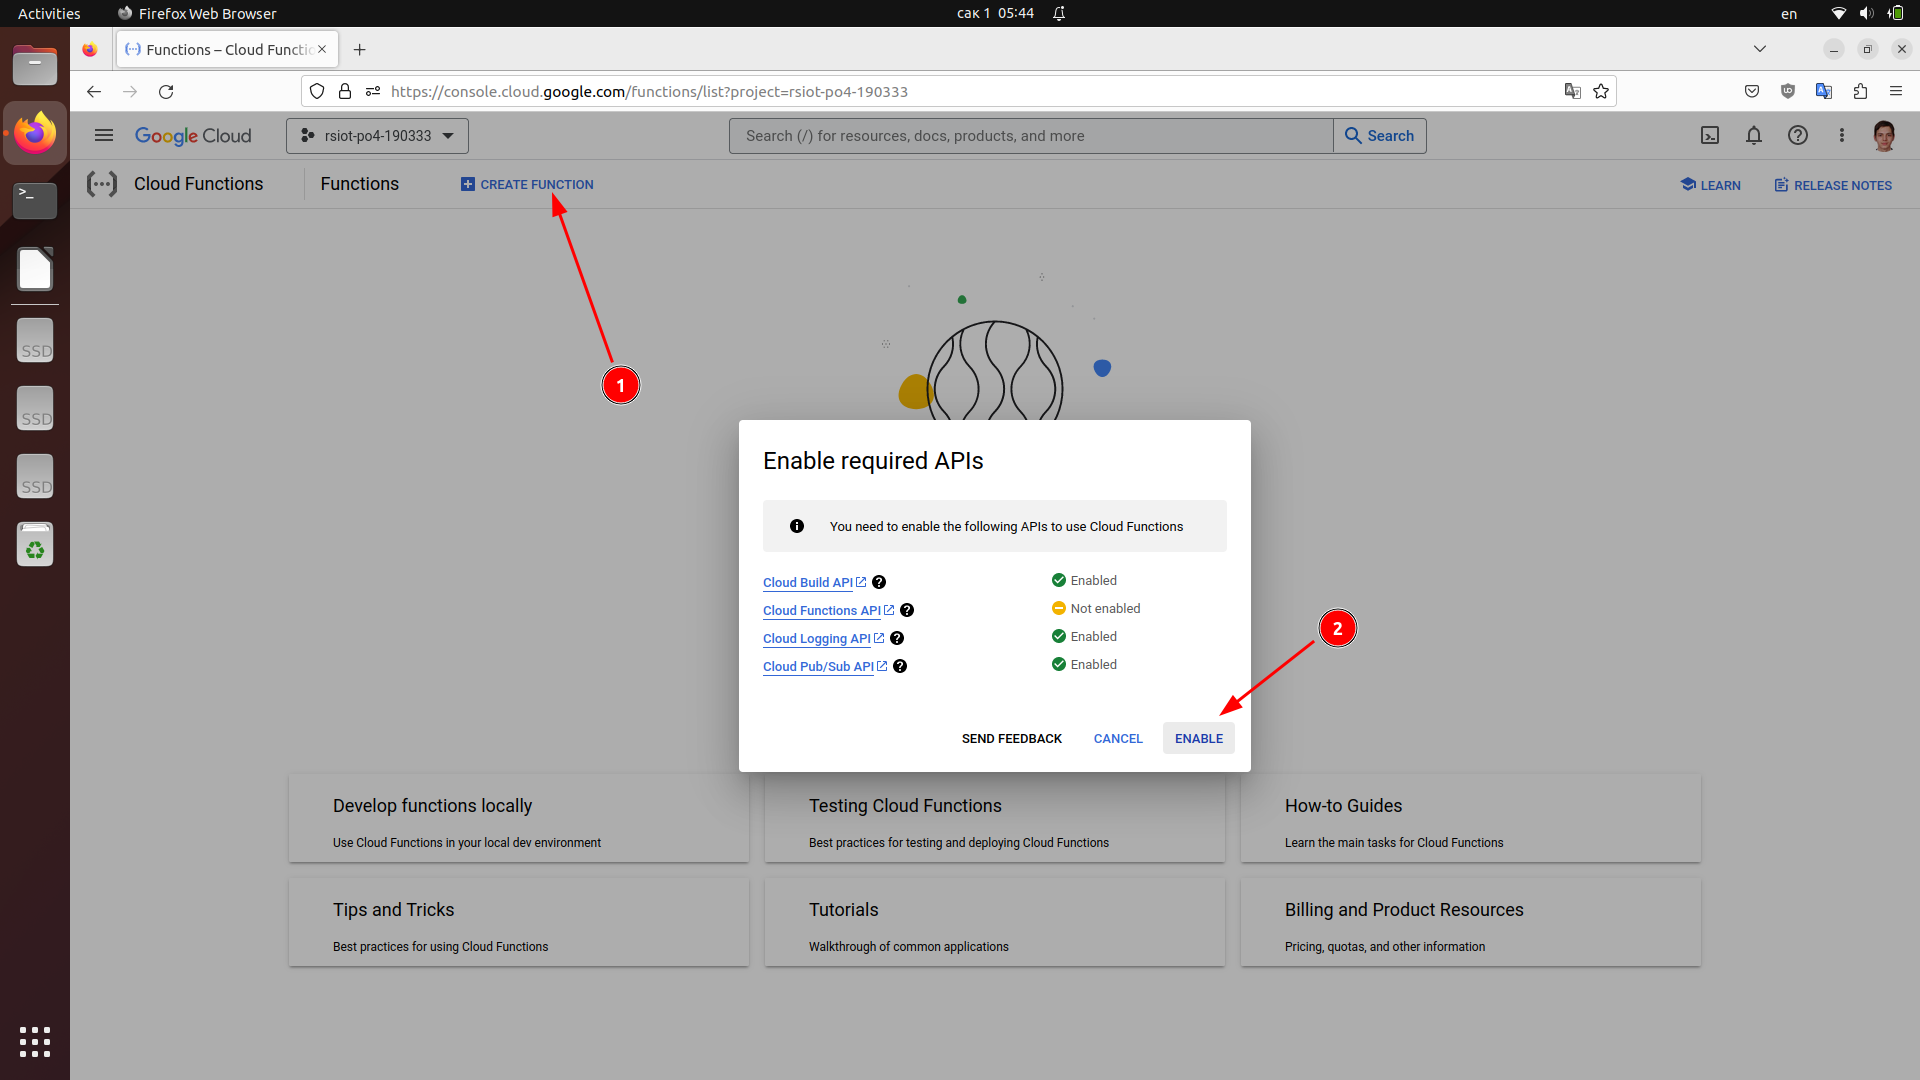
\includegraphics[width=10cm]
    {images/GoogleCloudFunctions/2023-03-01_05-44-49.png}
    \caption{\_}
    \label{fig:27}
  \end{figure}

  \newpage
  Function name: \underline{ms4} (см. рисунок~\ref{fig:28}).

  Authentification: \underline{Allow unauthenticated invocations} (см. рисунок~\ref{fig:28}).

  Require HTTPS: \underline{false} (см. рисунок~\ref{fig:28}).

  Жму <<Save>> (см. рисунок~\ref{fig:28}).
  Жму <<NEXT>> (см. рисунок~\ref{fig:28}).

  \begin{figure}[!h]
    \centering
    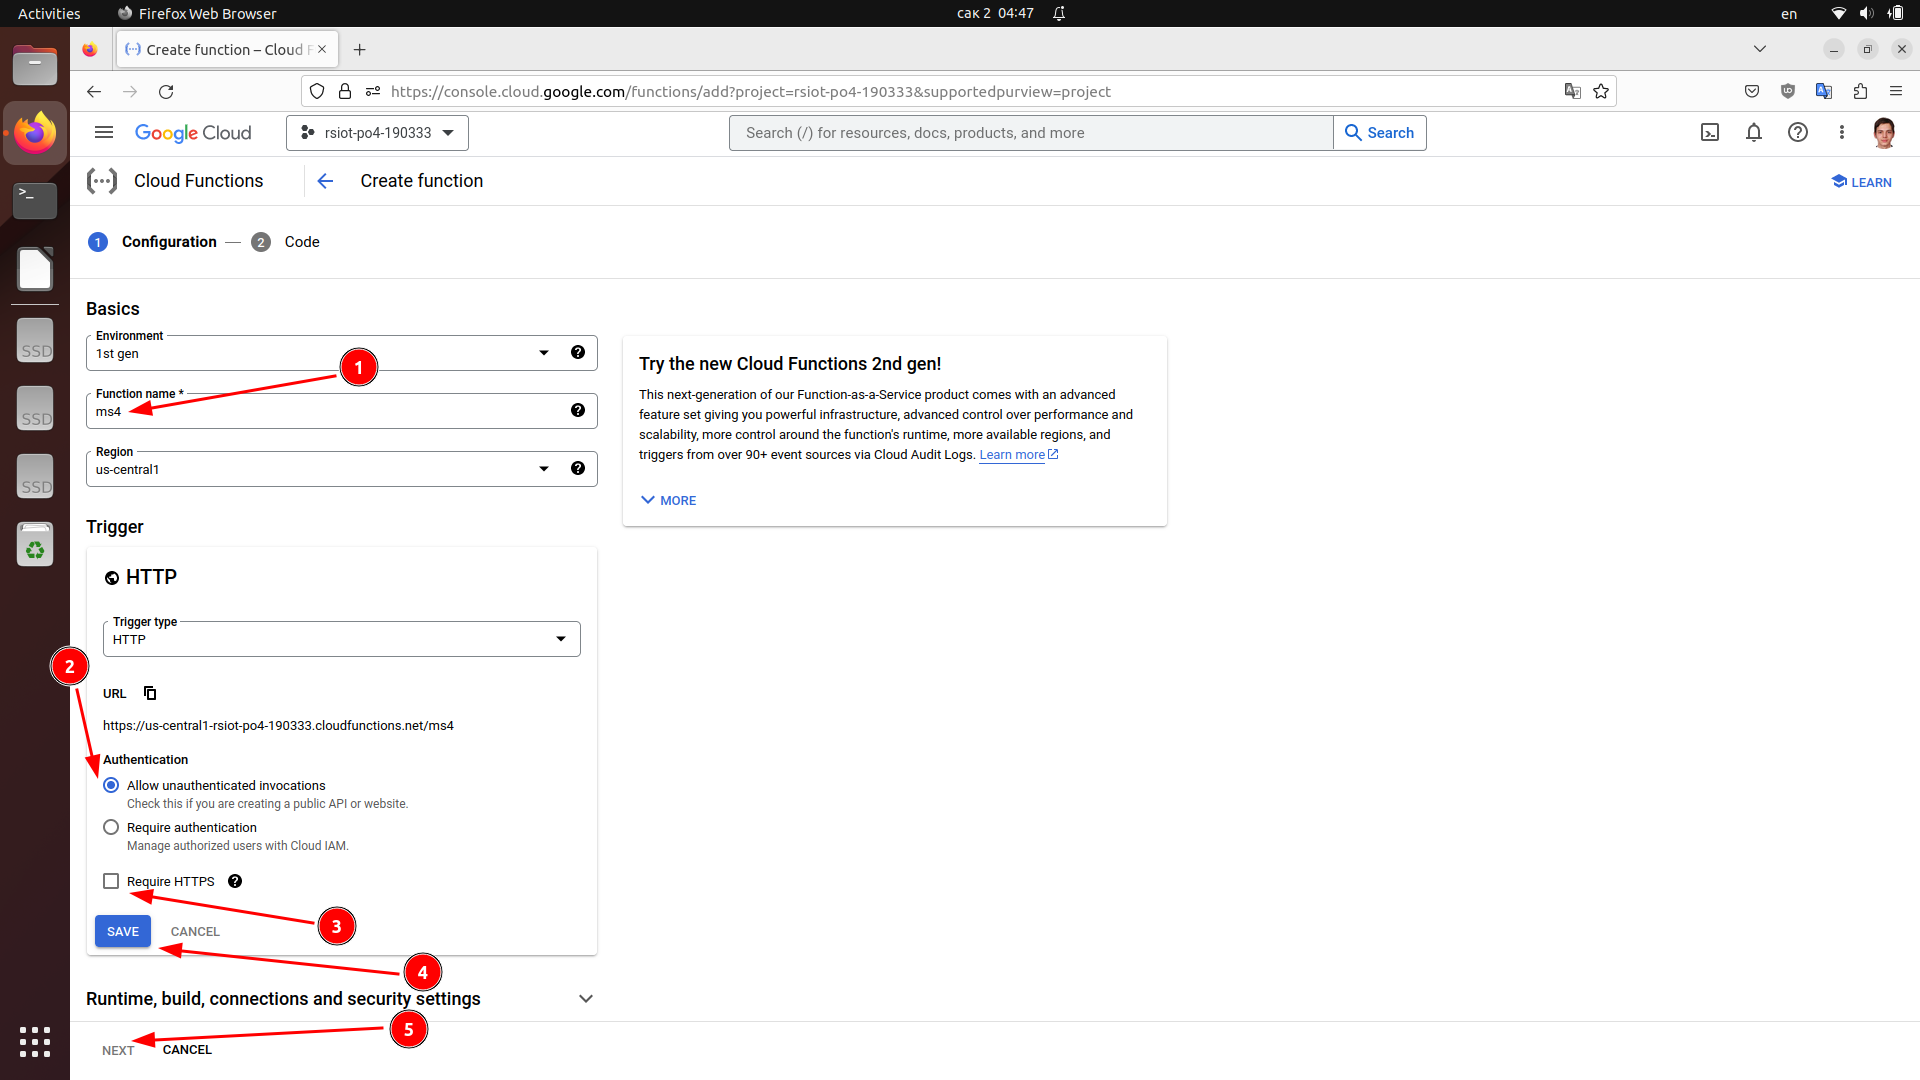
\includegraphics[width=10cm]
    {images/GoogleCloudFunctions/2023-03-02_04-48-52.png}
    \caption{\_}
    \label{fig:28}
  \end{figure}

  Выбираю файл package.json. Вставляю код (см. рисунок~\ref{fig:29}).

  Выбираю файл index.js. Вставляю код. Жму <<DEPLOY>> (см. рисунок~\ref{fig:30}).

  \begin{figure}[!h]
    \centering
  
    \begin{minipage}{0.49\textwidth}
      \centering
  
      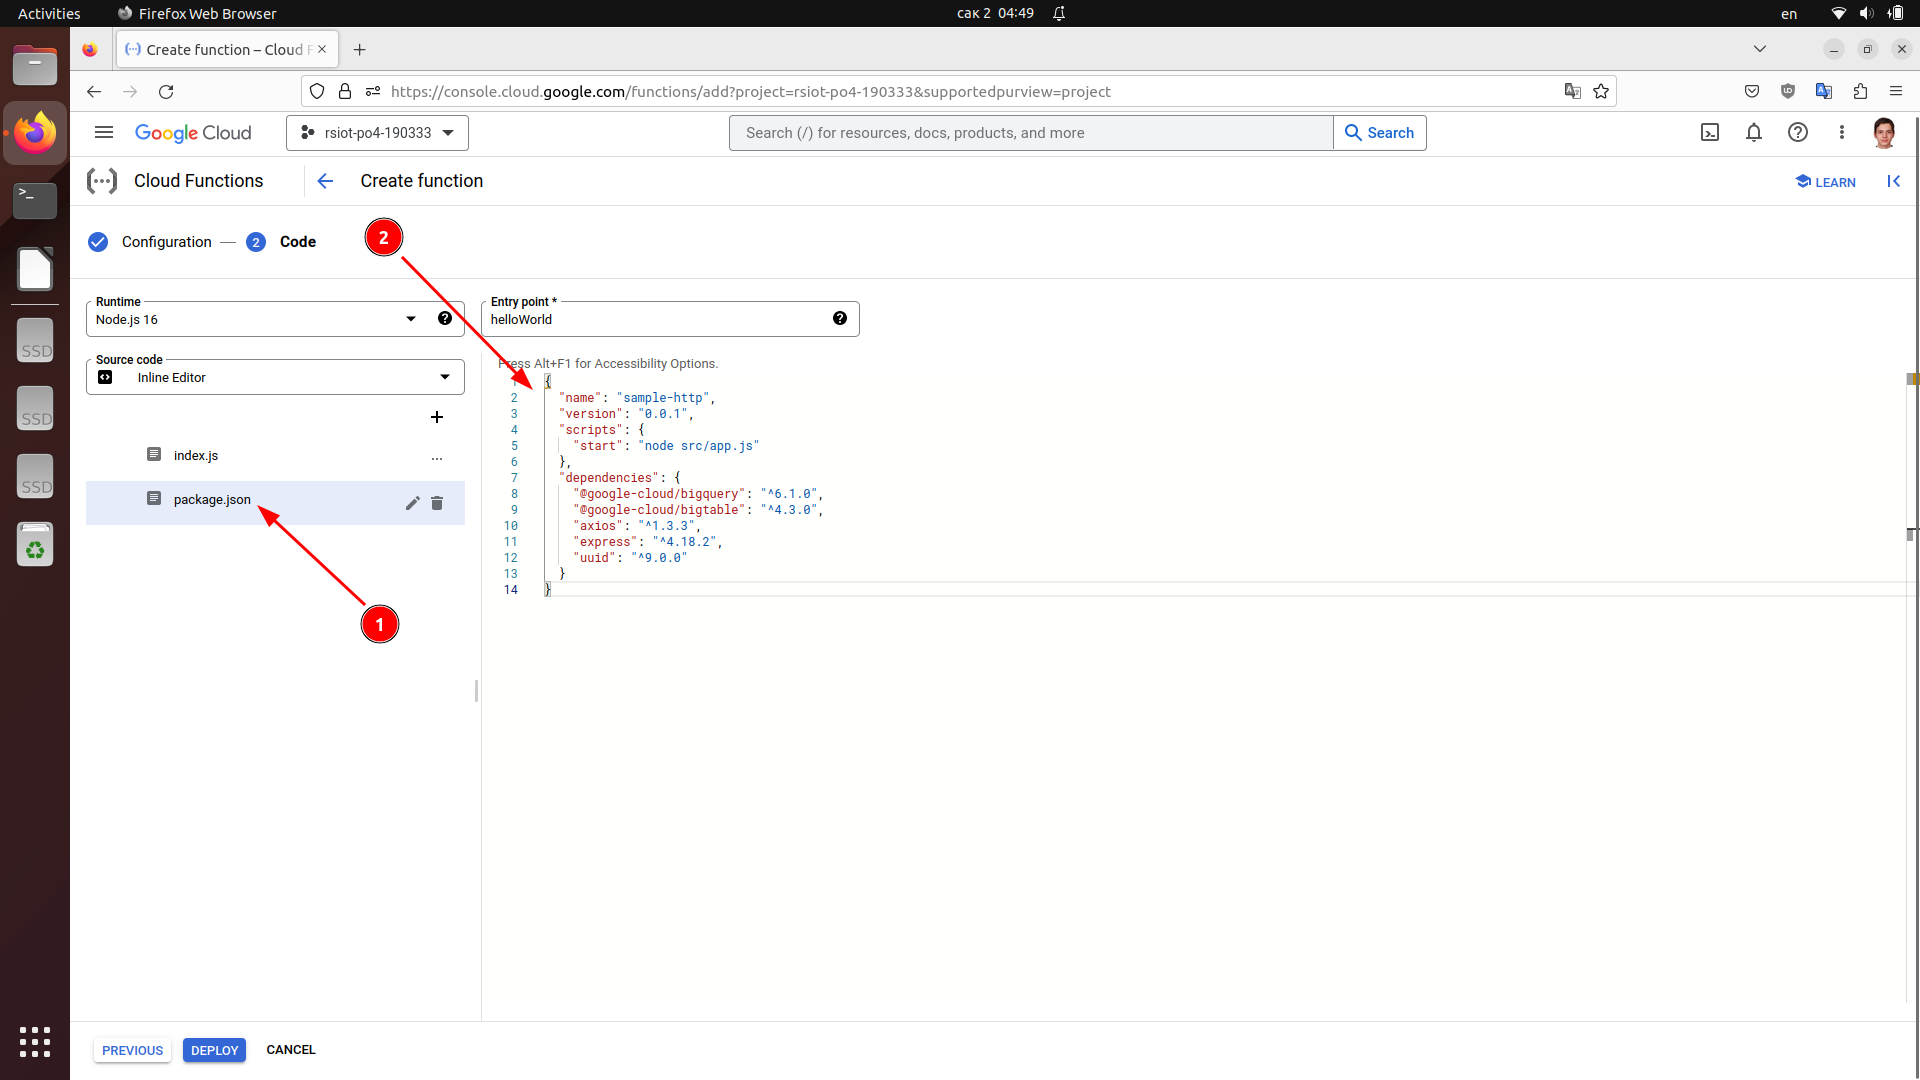
\includegraphics[height=5cm]
      {images/GoogleCloudFunctions/2023-03-02_04-50-11.png}
  
      \caption{\_}
  
      \label{fig:29}
    \end{minipage}
    \begin{minipage}{0.49\textwidth}
      \centering
  
      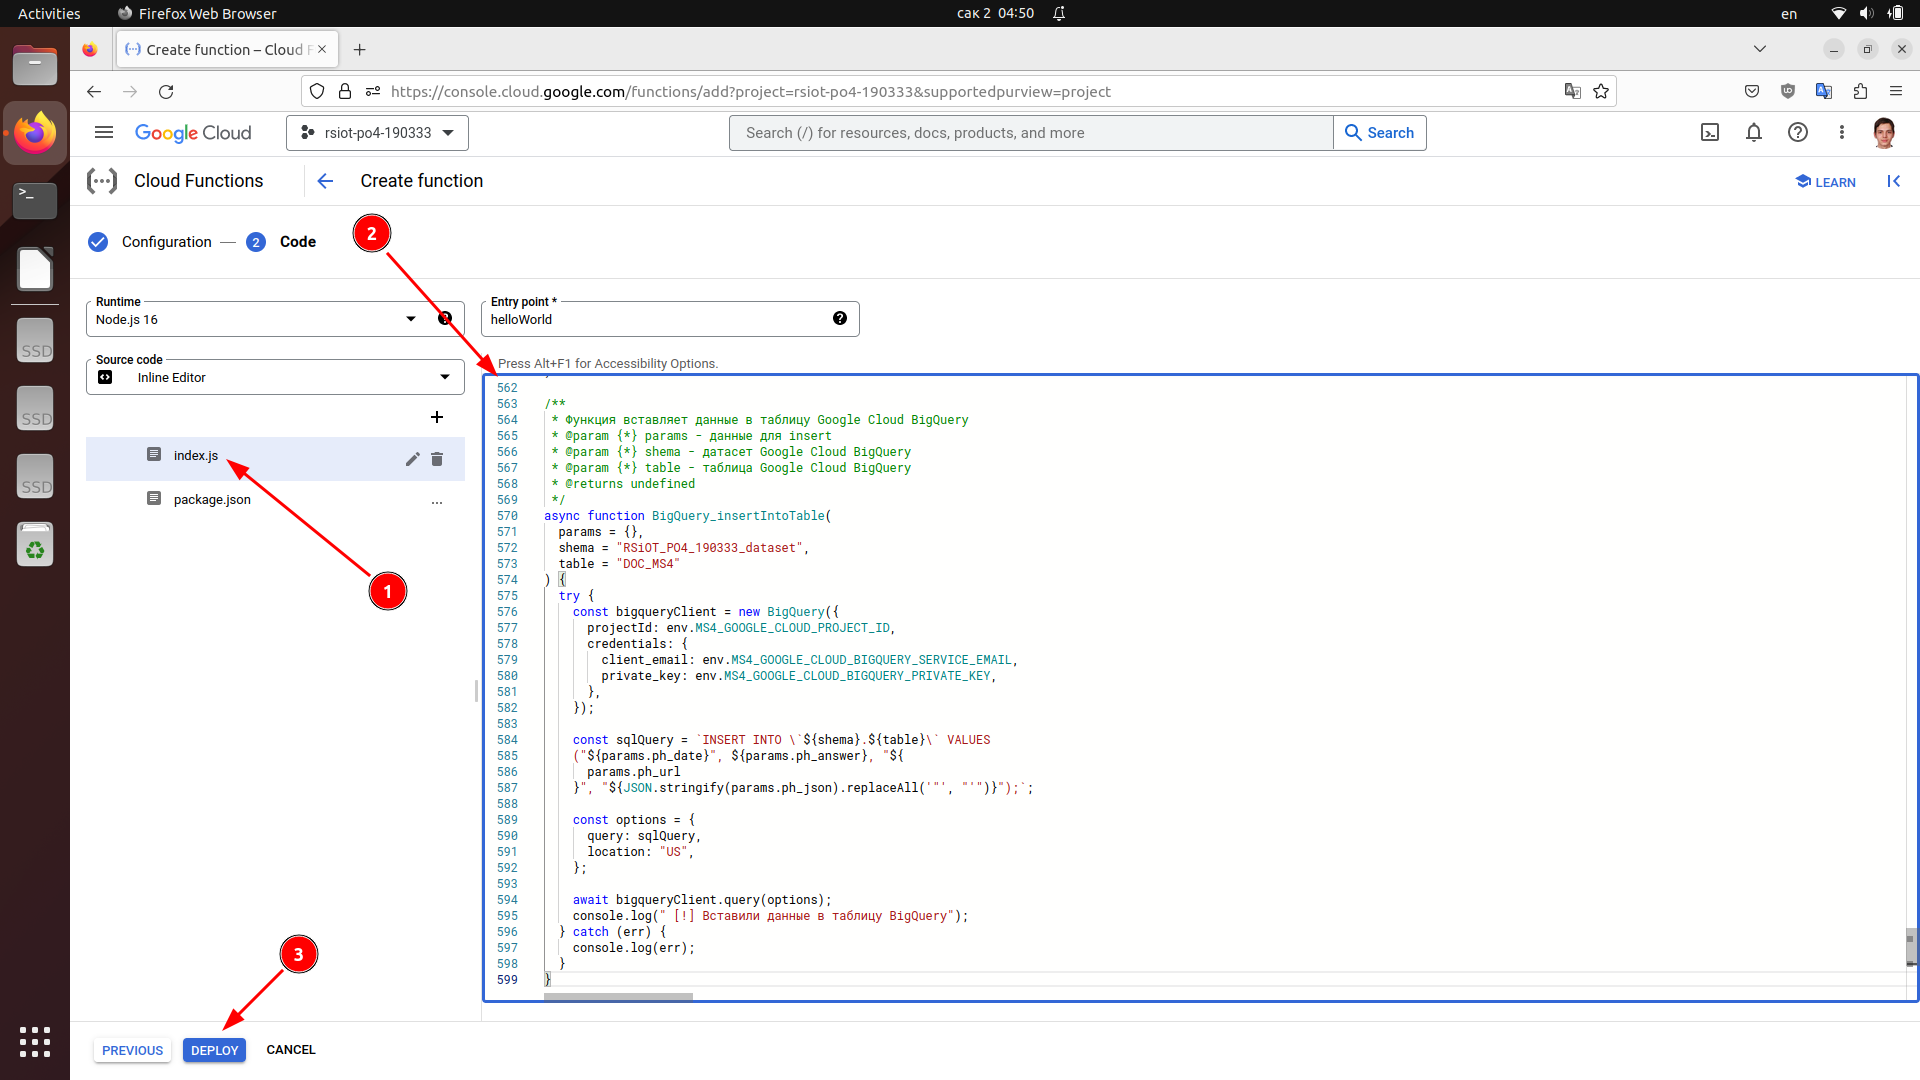
\includegraphics[height=5cm]
      {images/GoogleCloudFunctions/2023-03-02_04-51-27.png}
  
      \caption{\_}
  
      \label{fig:30}
    \end{minipage}
  \end{figure}

  % \newpage

  \lstinputlisting[
    frame=single,
    rulecolor=\color{blue},
  ]{../sources/MS4/package.json}

  \newpage

  \lstinputlisting[
    frame=single,
    rulecolor=\color{blue},
  ]{../sources/MS4/src/index.js}

  Файл app.js не нужно загружать на Google Cloud Functions. Он нужен для того, чтобы эмулировать сервер,
  который вызываем командой <<node src/app.js>> или <<npm run start>>.

  \lstinputlisting[
    frame=single,
    rulecolor=\color{blue},
  ]{../sources/MS4/src/app.js}

  \newpage

  Жму <<TRIGGER>> (см. рисунок~\ref{fig:31}).

  Жду пока загрузится функций (должна появится зелённая галочка) (см. рисунок~\ref{fig:31}).

  Перехожу по ссылке-треггеру (см. рисунок~\ref{fig:31}).

  \begin{figure}[!h]
    \centering
    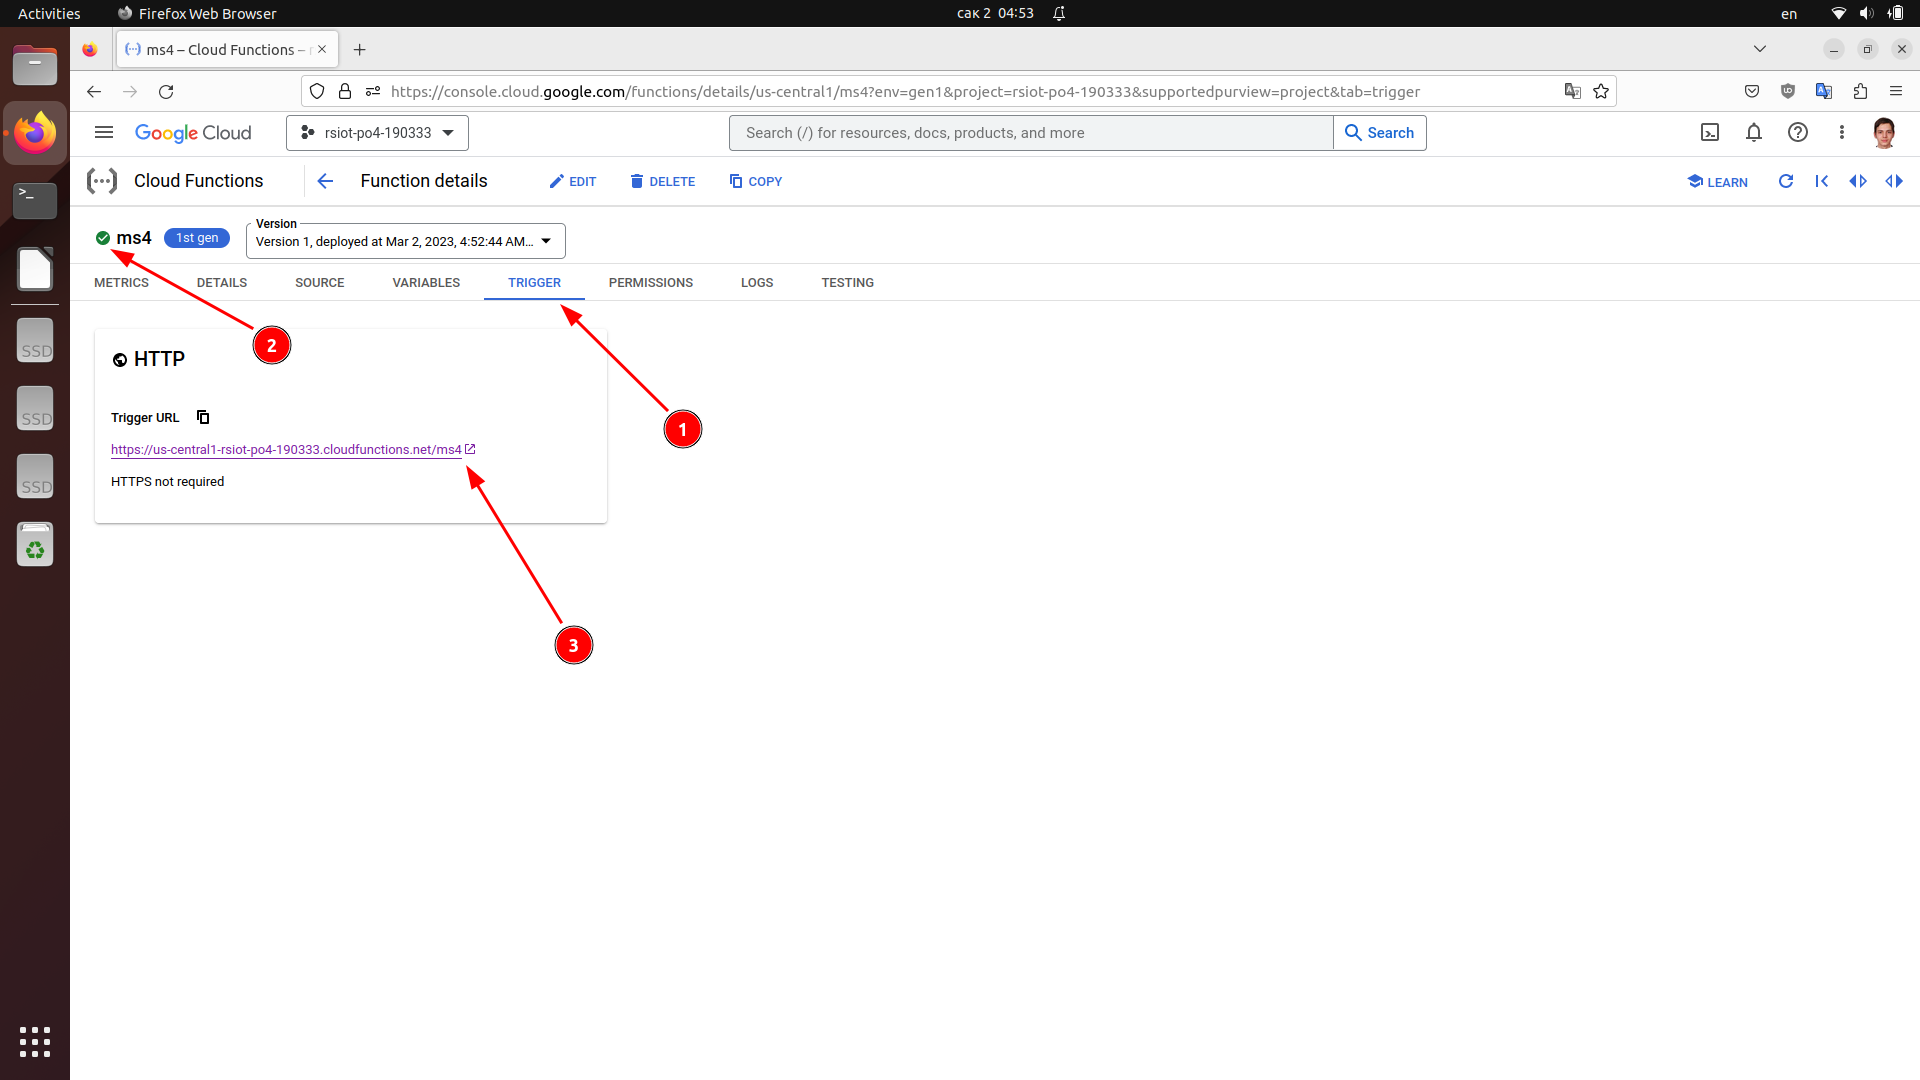
\includegraphics[width=18cm]
    {images/GoogleCloudFunctions/2023-03-02_04-54-09.png}
    \caption{\_}
    \label{fig:31}
  \end{figure}

  Результат, который вернул Google Cloud Functions - JSON с даными от MS2, выборка с таблицы BigTable
  и выборка с таблицы BigQuery (см. рисунок~\ref{fig:32}).

  \begin{figure}[!h]
    \centering
    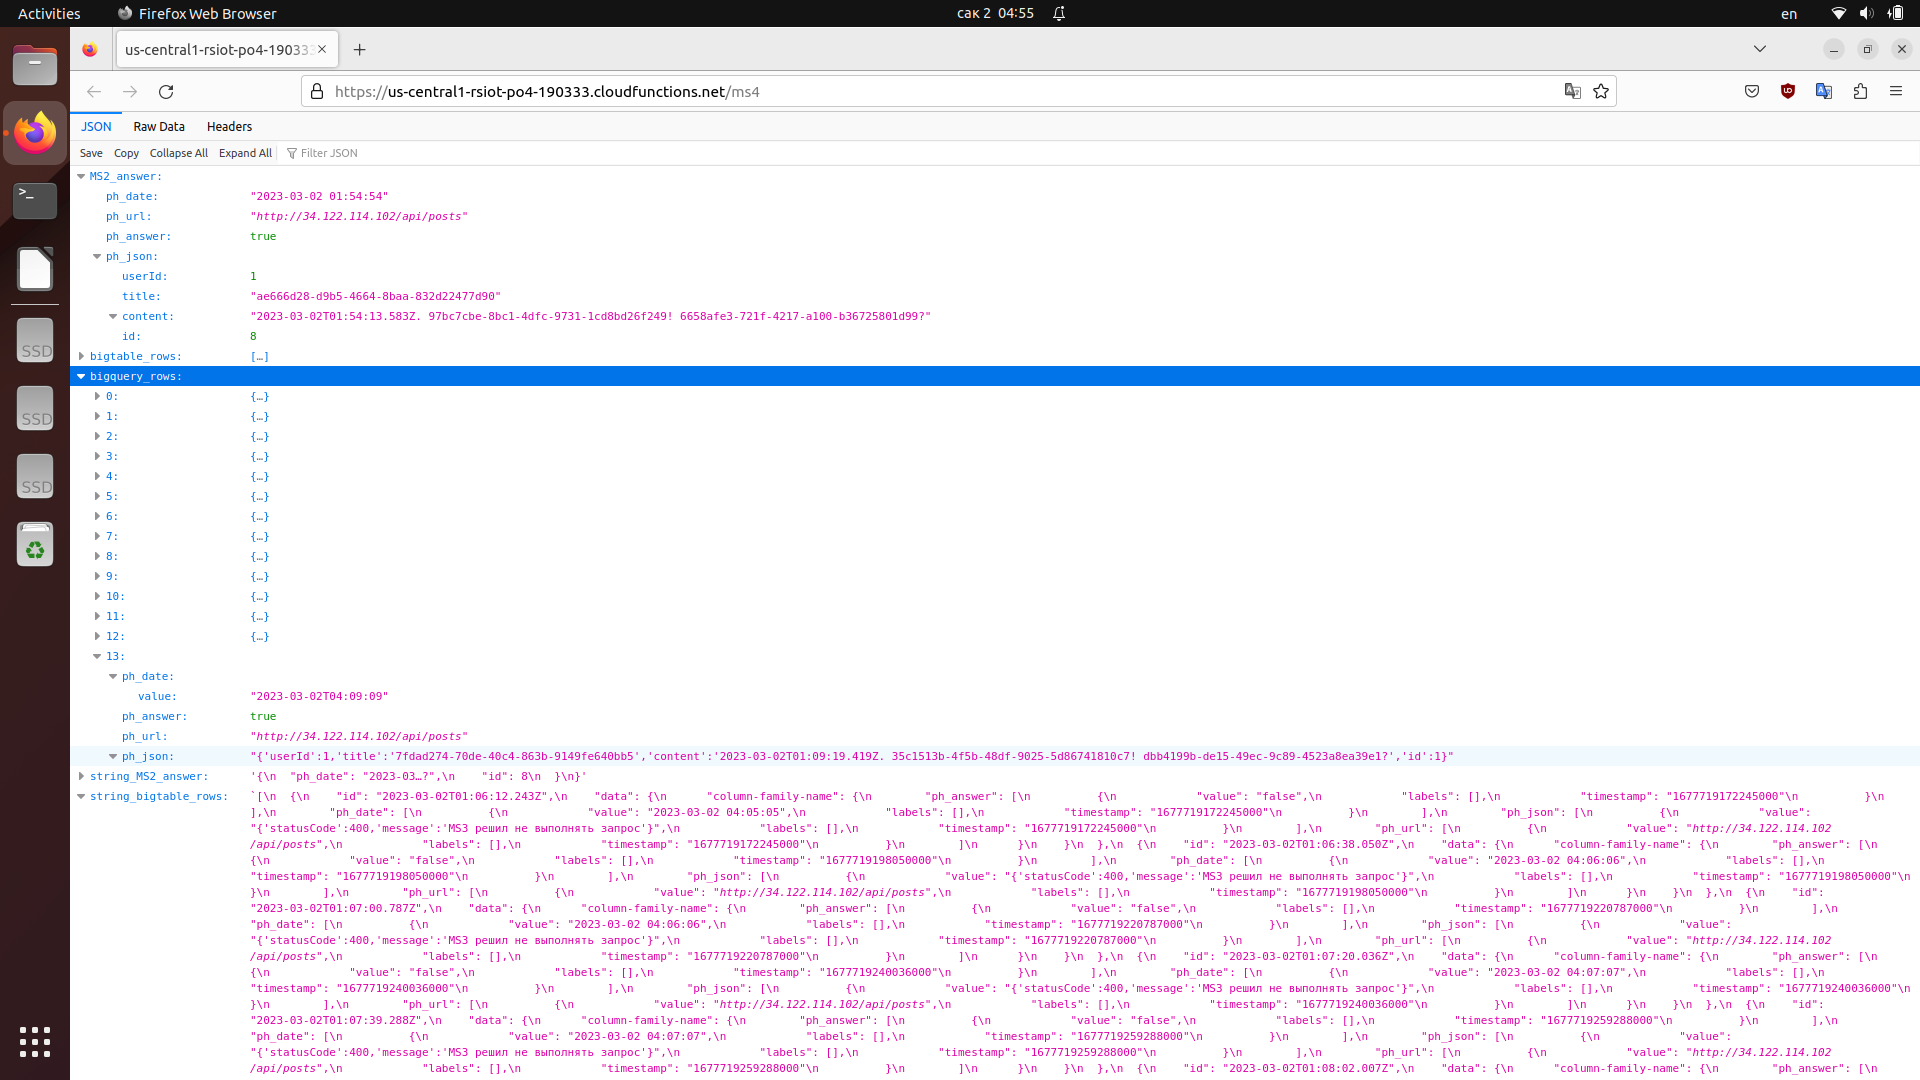
\includegraphics[width=18cm]
    {images/GoogleCloudFunctions/2023-03-02_04-55-58.png}
    \caption{\_}
    \label{fig:32}
  \end{figure}

  \newpage

  \begin{center}
    \textbf{Создание запланированной задачи в Google Cloud Scheduler}
  \end{center}

  Заходим на сайт Google Cloud Console \cite{GoogleCloudConsole} (см. рисунок~\ref{fig:33}).

  Menu > Cloud Scheduler \cite{GoogleCloudScheduler} (см. рисунок~\ref{fig:33}).

  Жму <<CREATE JOB>> (см. рисунок~\ref{fig:34}).

  \begin{figure}[!h]
    \centering
  
    \begin{minipage}{0.49\textwidth}
      \centering
  
      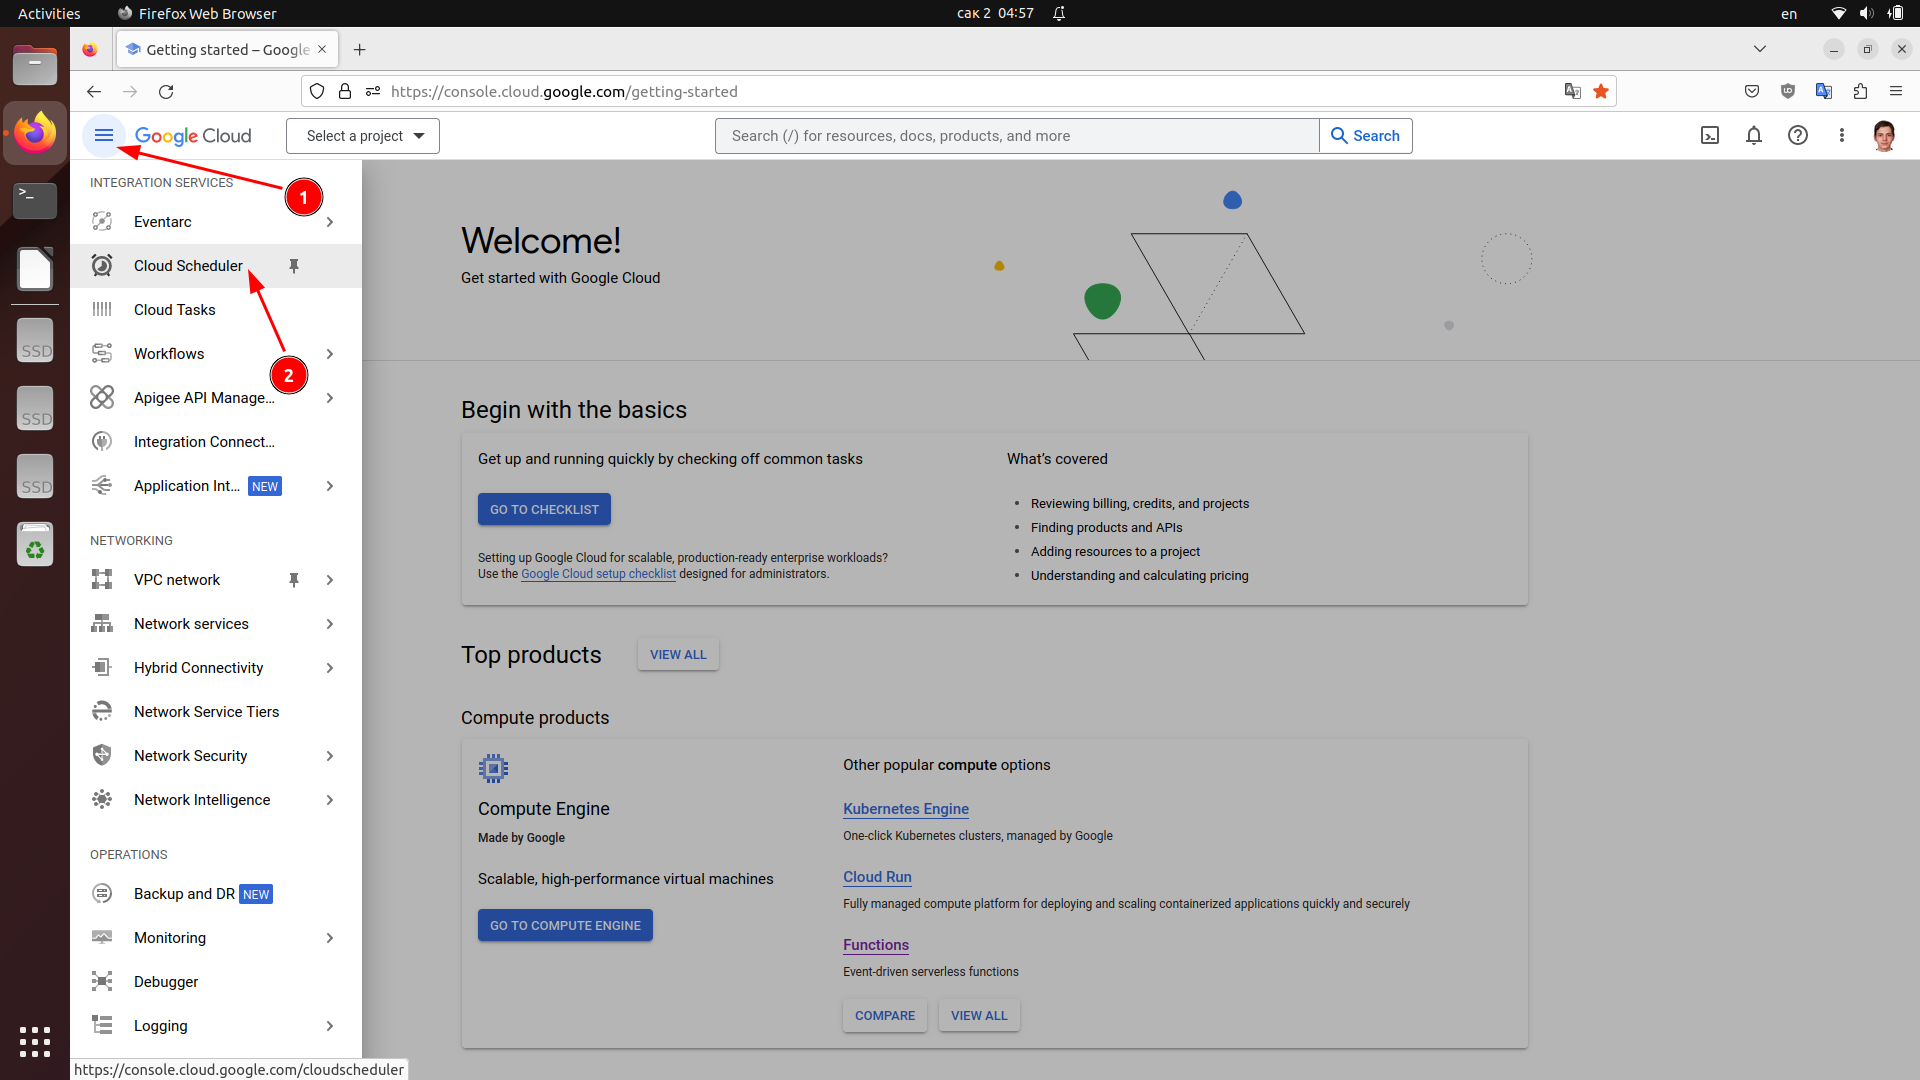
\includegraphics[height=5cm]
      {images/GoogleCloudScheduler/2023-03-02_04-58-10.png}
  
      \caption{\_}
  
      \label{fig:33}
    \end{minipage}
    \begin{minipage}{0.49\textwidth}
      \centering
  
      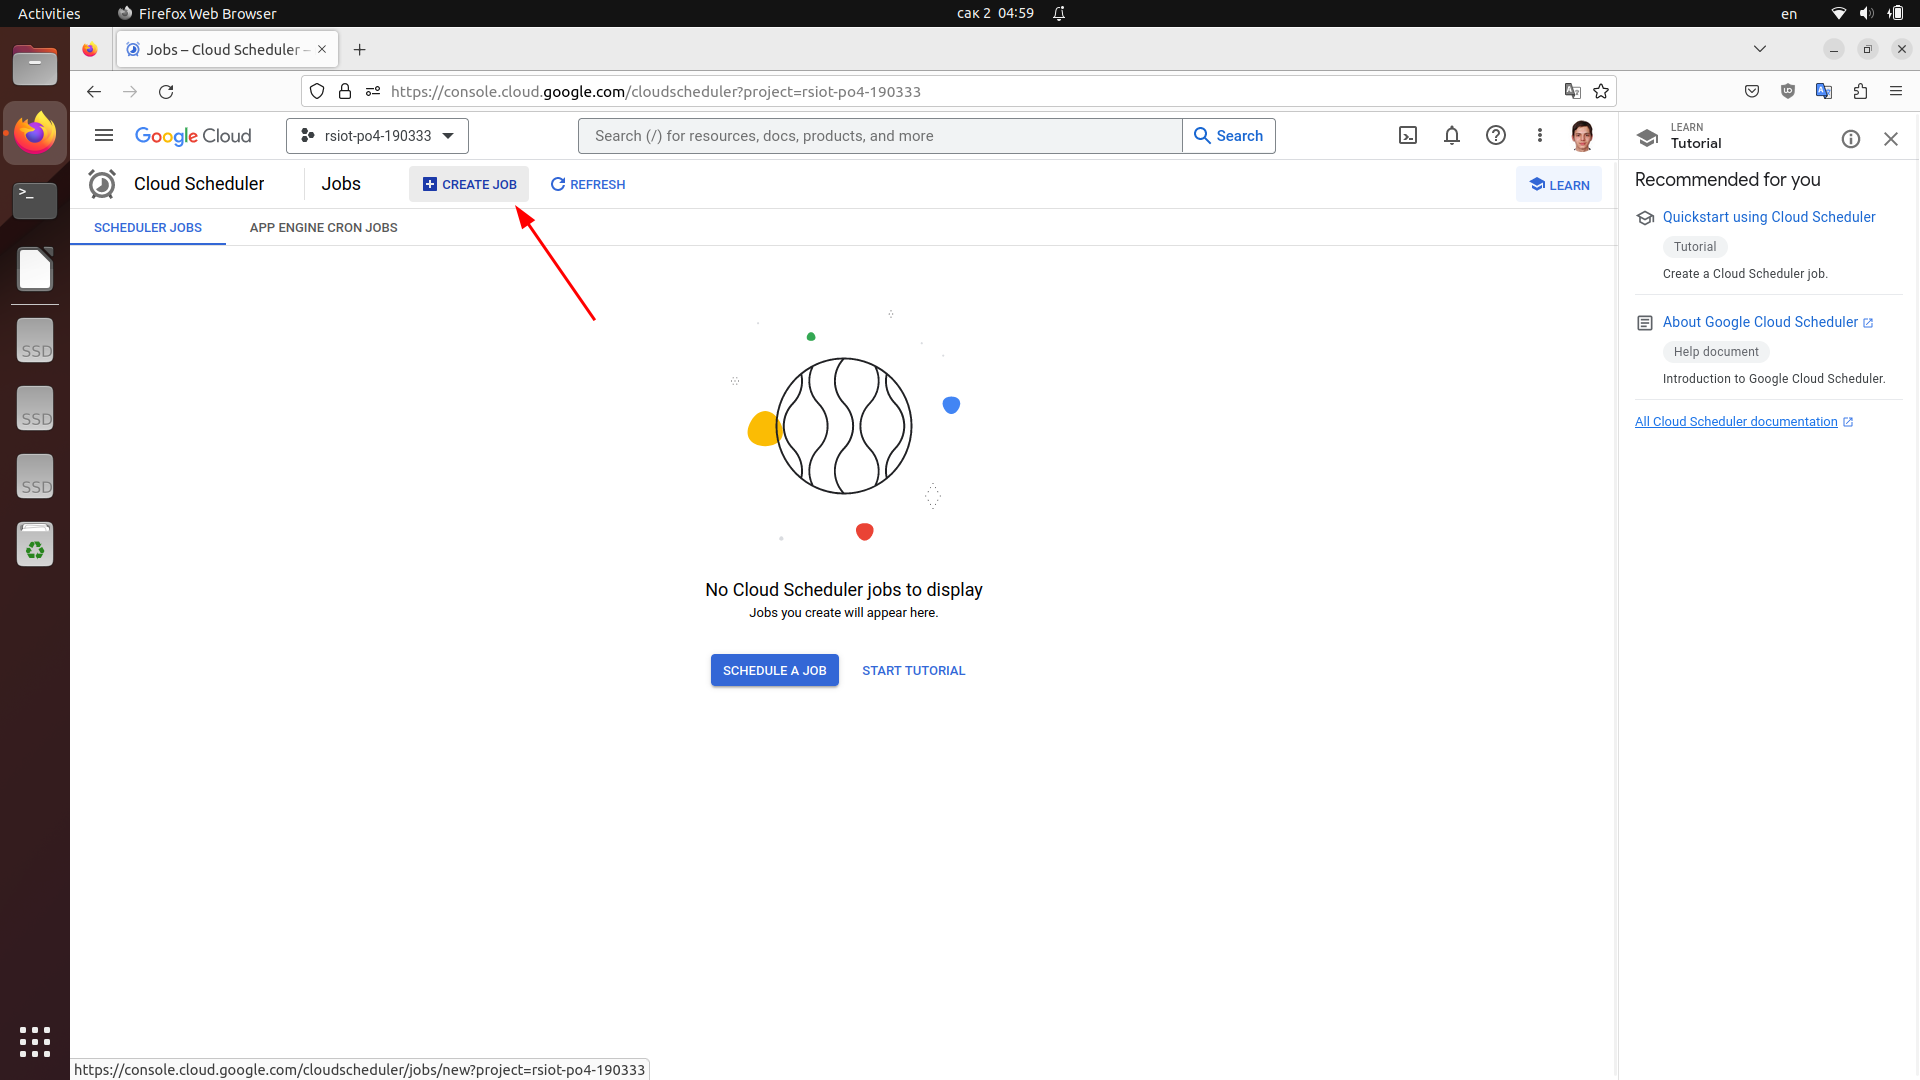
\includegraphics[height=5cm]
      {images/GoogleCloudScheduler/2023-03-02_04-59-19.png}
  
      \caption{\_}
  
      \label{fig:34}
    \end{minipage}
  \end{figure}

  Name: \underline{MS4-run-every-minute} (см. рисунок~\ref{fig:35}).

  Frequency: \underline{* * * * *} (см. рисунок~\ref{fig:35}).

  Timezone: \underline{Coordinated Universal Time (UTC)} (см. рисунок~\ref{fig:35}).

  Жму <<CONTINUE>> (см. рисунок~\ref{fig:35}).

  \begin{figure}[!h]
    \centering
    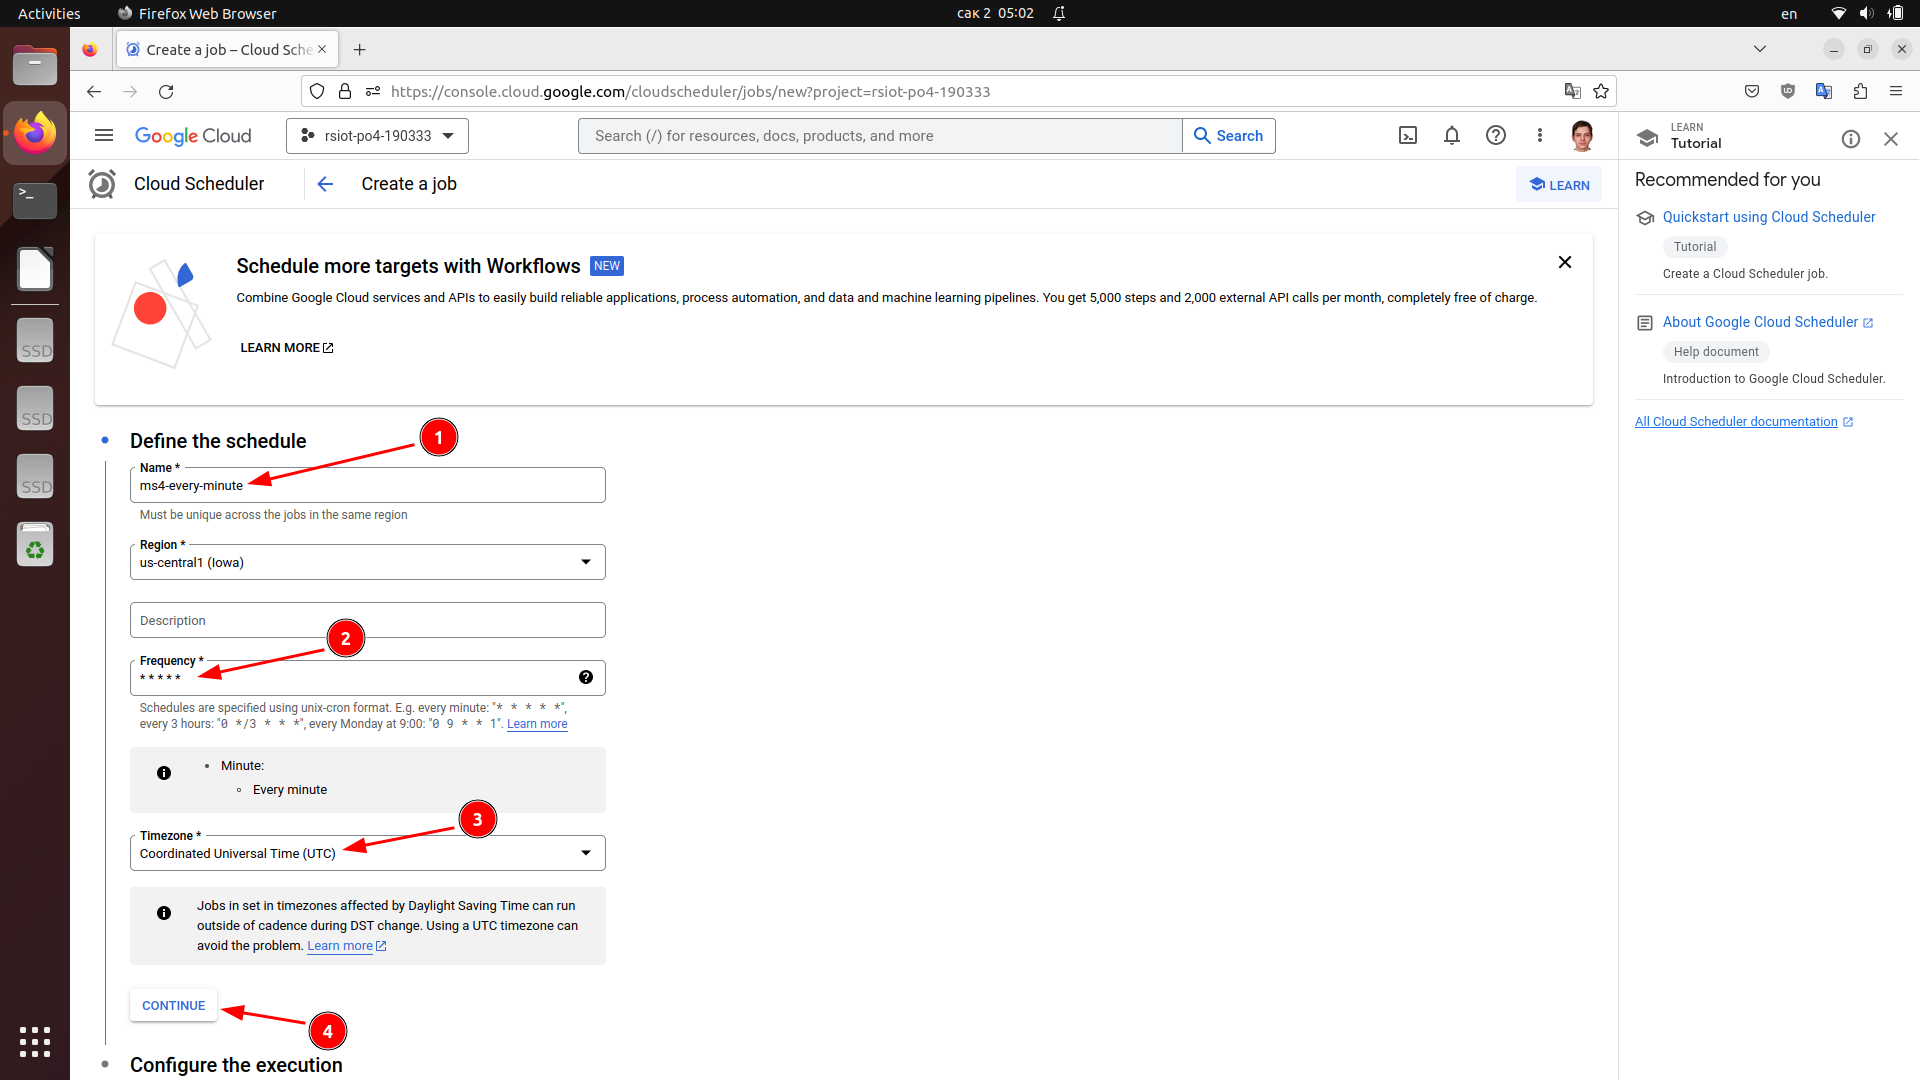
\includegraphics[width=18cm]
    {images/GoogleCloudScheduler/2023-03-02_05-02-58.png}
    \caption{\_}
    \label{fig:35}
  \end{figure}

  \newpage

  Target type: \underline{HTTP} (см. рисунок~\ref{fig:36}).

  URL: \underline{https://us-central1-rsiot-po4-190333.cloudfunctions.net/ms4}
  (вставить триггер-ссылку от Google Cloud Functions) (см. рисунок~\ref{fig:36}).

  Жму <<CONTINUE>> (см. рисунок~\ref{fig:36}).

  \begin{figure}[!h]
    \centering
    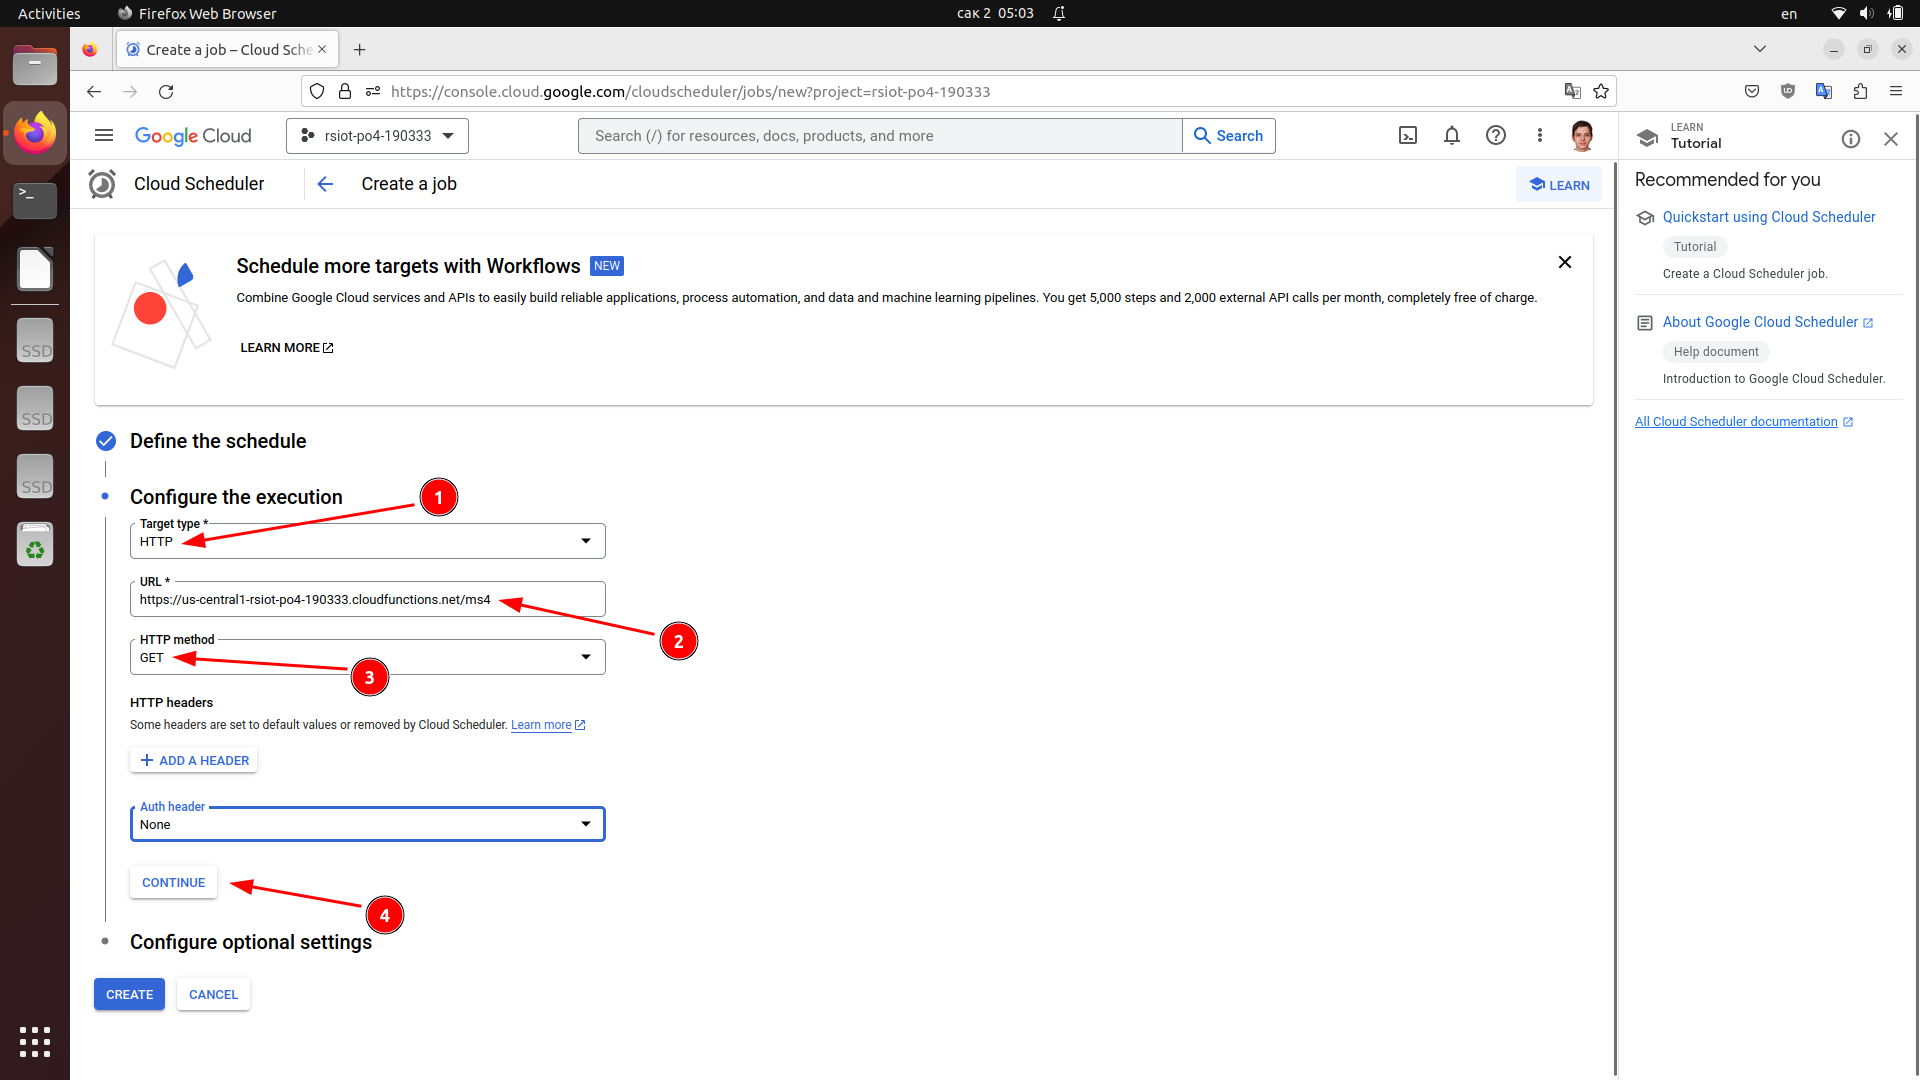
\includegraphics[width=10cm]
    {images/GoogleCloudScheduler/2023-03-02_05-04-22.png}
    \caption{\_}
    \label{fig:36}
  \end{figure}

  Жму <<CREATE>> (см. рисунок~\ref{fig:37}).

  \begin{figure}[!h]
    \centering
    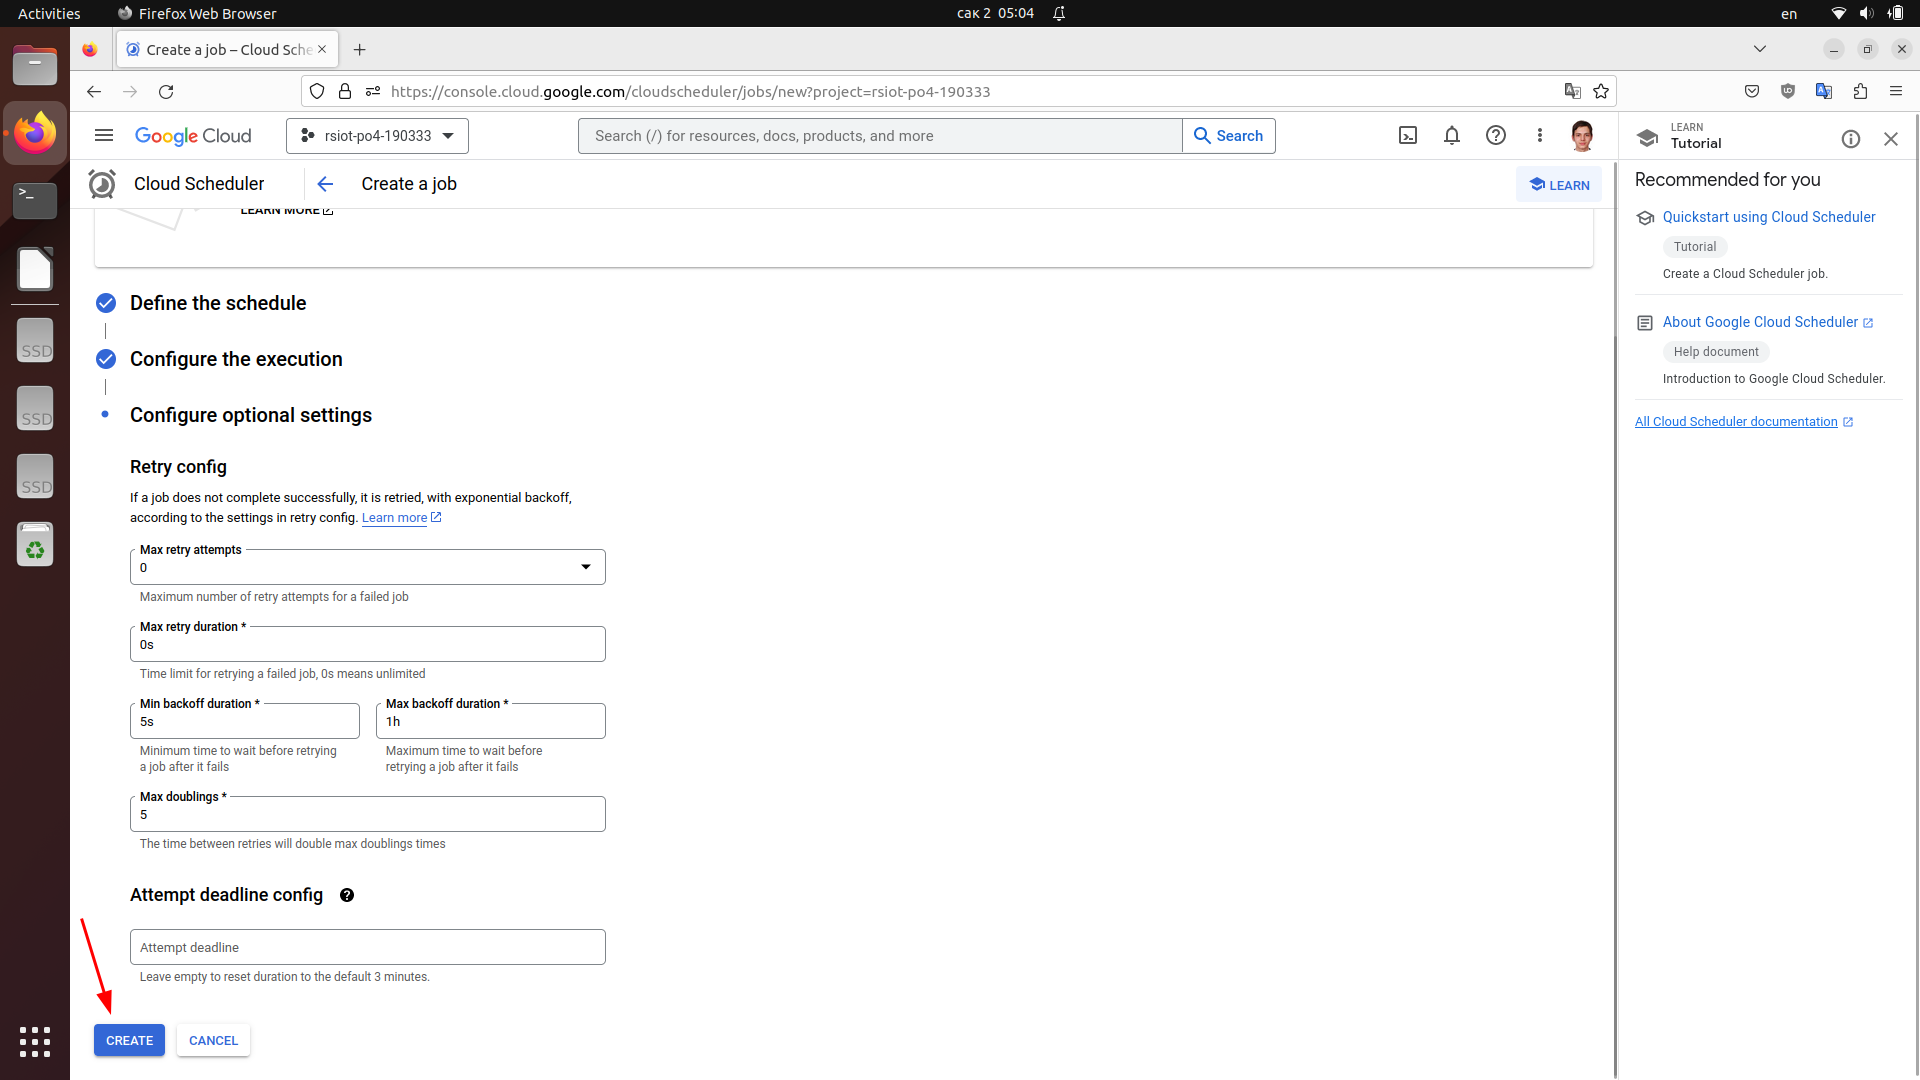
\includegraphics[width=10cm]
    {images/GoogleCloudScheduler/2023-03-02_05-04-46.png}
    \caption{\_}
    \label{fig:37}
  \end{figure}

  Функция должна запускаться каждую минуту. Спустя время видим галочку об успешном запуске (см. рисунок~\ref{fig:38}).

  \begin{figure}[!h]
    \centering
    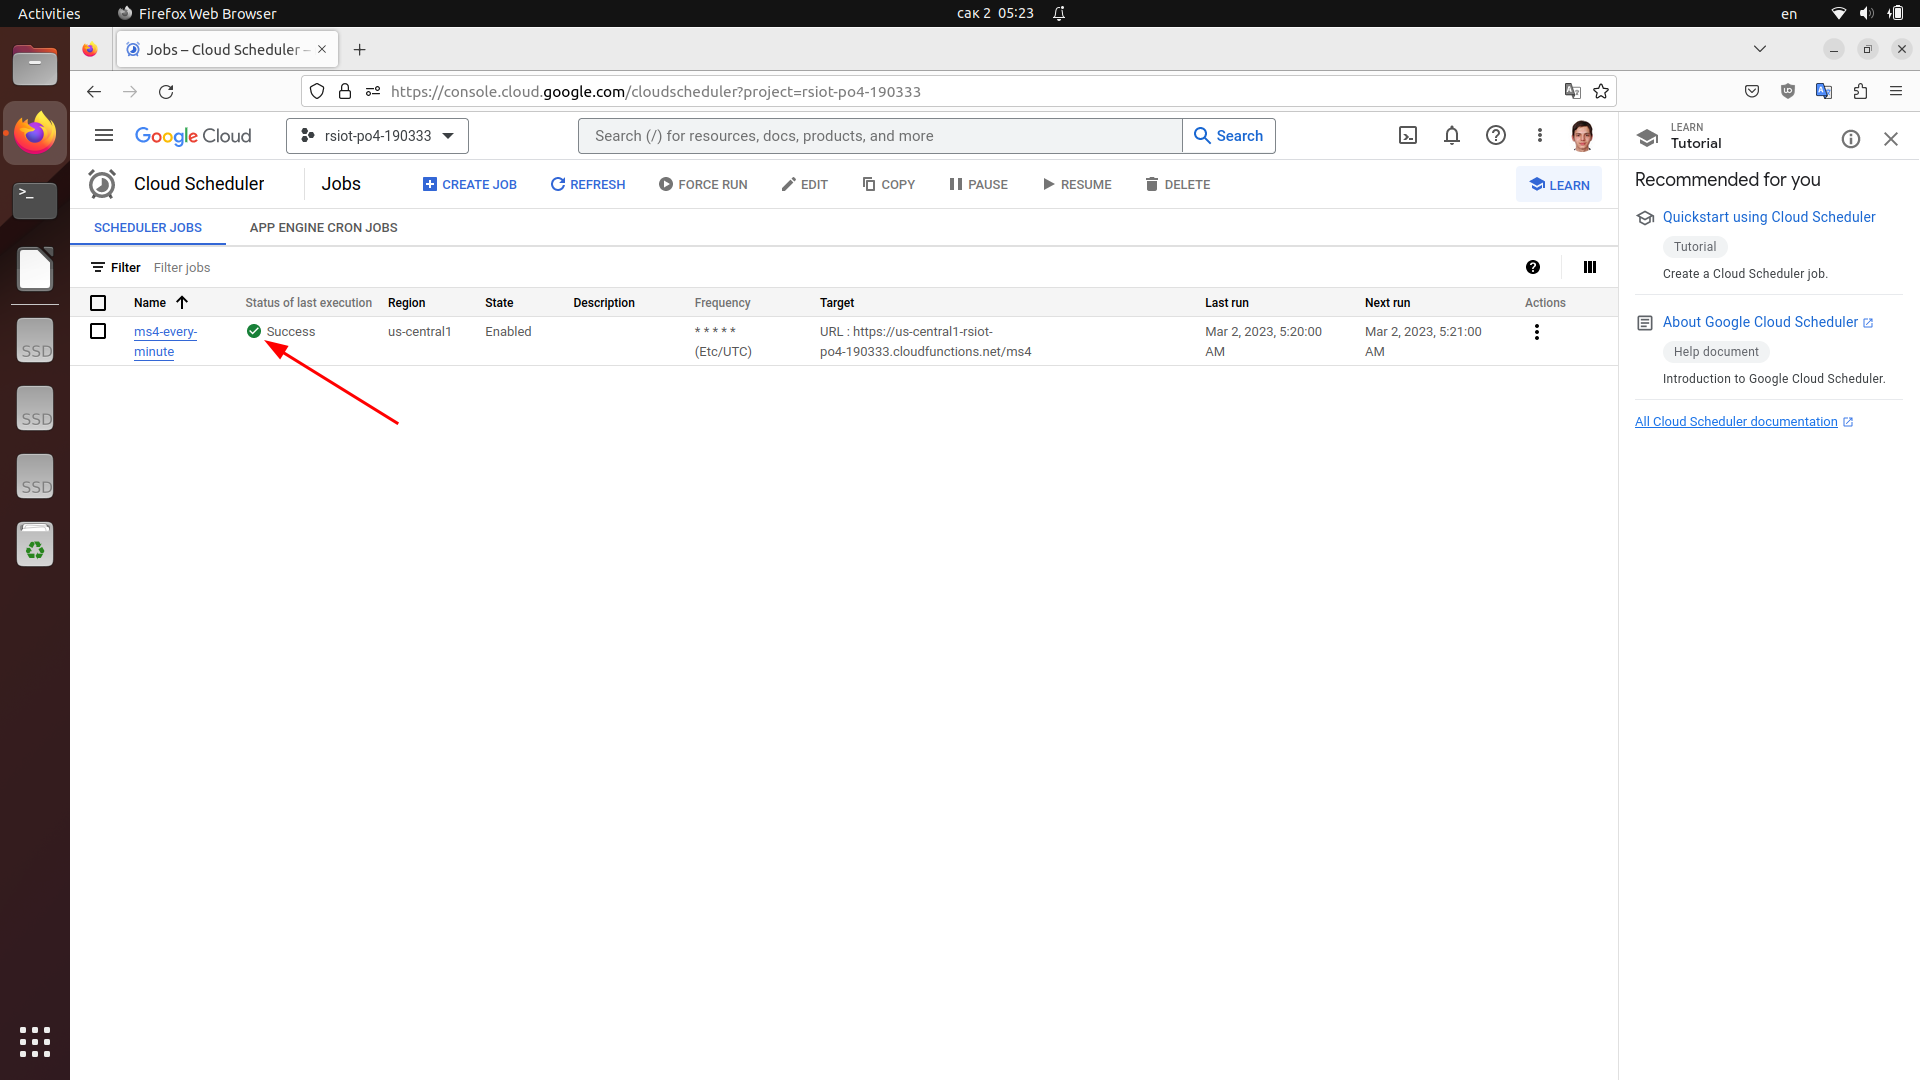
\includegraphics[width=10cm]
    {images/GoogleCloudScheduler/2023-03-02_05-23-29.png}
    \caption{\_}
    \label{fig:38}
  \end{figure}

  В логах (Google Cloud Logging) можно увидеть (см. рисунок~\ref{fig:39}), что Google Cloud Functions работает,
  так как происходит вставка Google Cloud BigTable, Google Cloud BigQuery.

  \begin{figure}[!h]
    \centering
    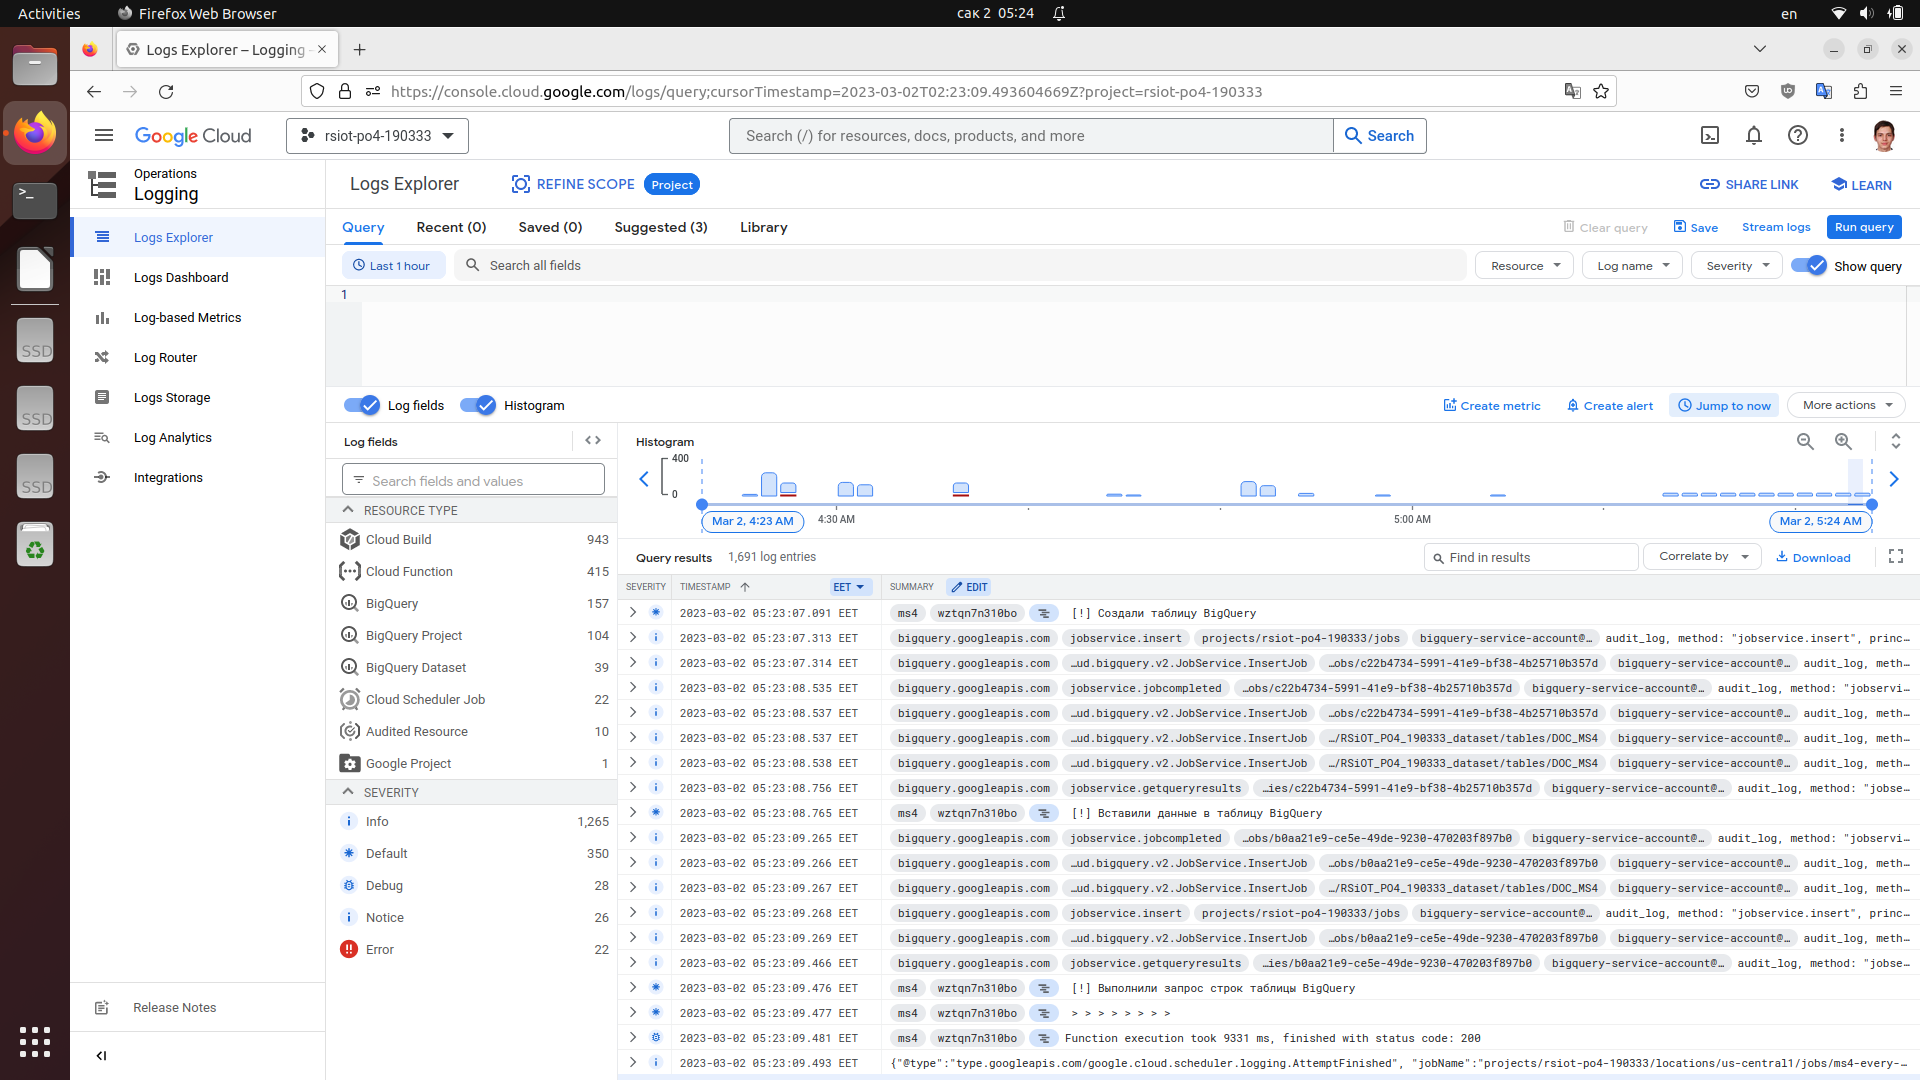
\includegraphics[width=16cm]
    {images/GoogleCloudScheduler/2023-03-02_05-24-13.png}
    \caption{\_}
    \label{fig:39}
  \end{figure}

  \begin{center}
    \textbf{Запрос в Google Cloud BigQuery через сайт}
  \end{center}


\begin{lstlisting}[
  language=sql,
  frame=single,
  rulecolor=\color{magenta},
  name={SQL команды по получению данных с таблицы Google Cloud BigQuery},
]
SELECT * FROM `RSiOT_PO4_190333_dataset.DOC_MS4`;
\end{lstlisting}

  Результат выборки из таблицы Google Cloud BigQuery \cite{GoogleCloudBigQuery} на рис.~\ref{fig:40}.

  \begin{figure}[!h]
    \centering
    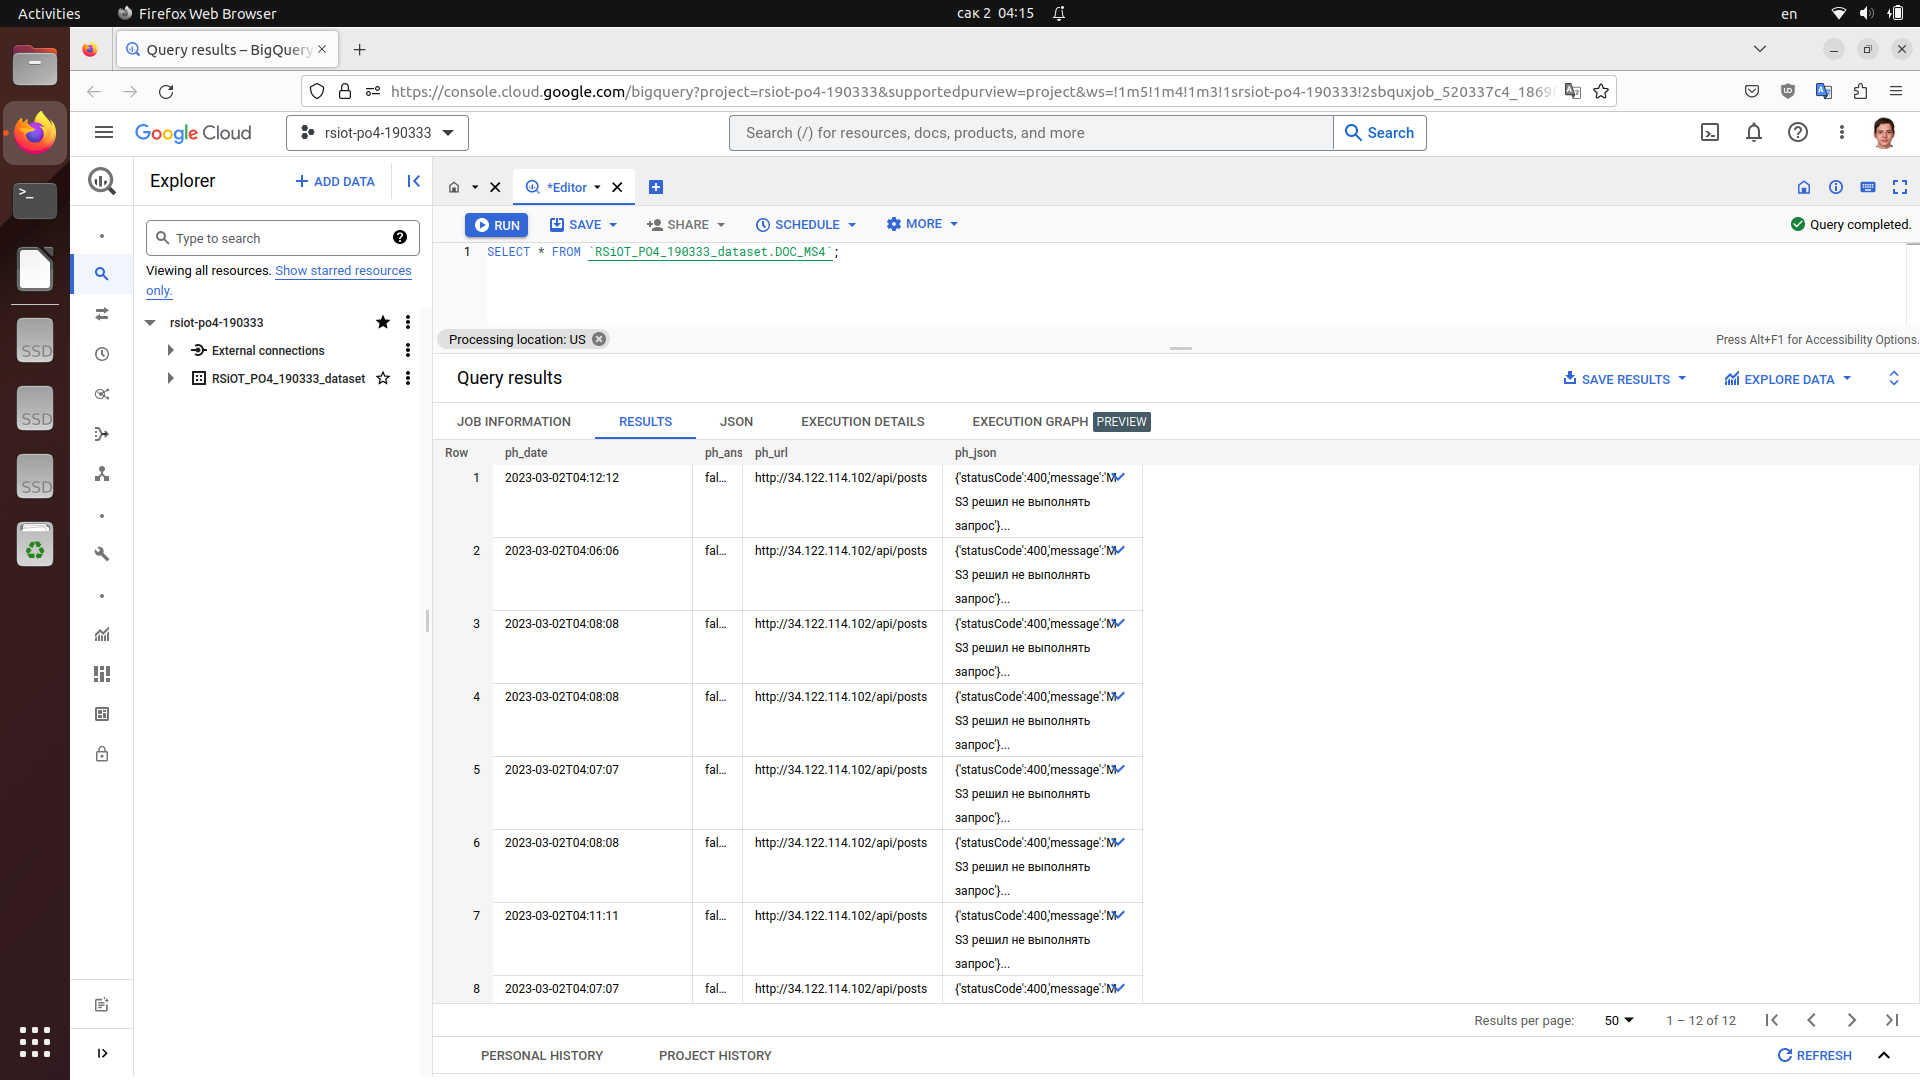
\includegraphics[width=16cm]
    {images/GoogleCloudBigQueryExplorer/2023-03-02_04-15-26.png}
    \caption{\_}
    \label{fig:40}
  \end{figure}

  \newpage
  Результат выборки из таблицы Google Cloud BigQuery \cite{GoogleCloudBigQuery} в виде JSON на рис.~\ref{fig:41}.

  \begin{figure}[!h]
    \centering
    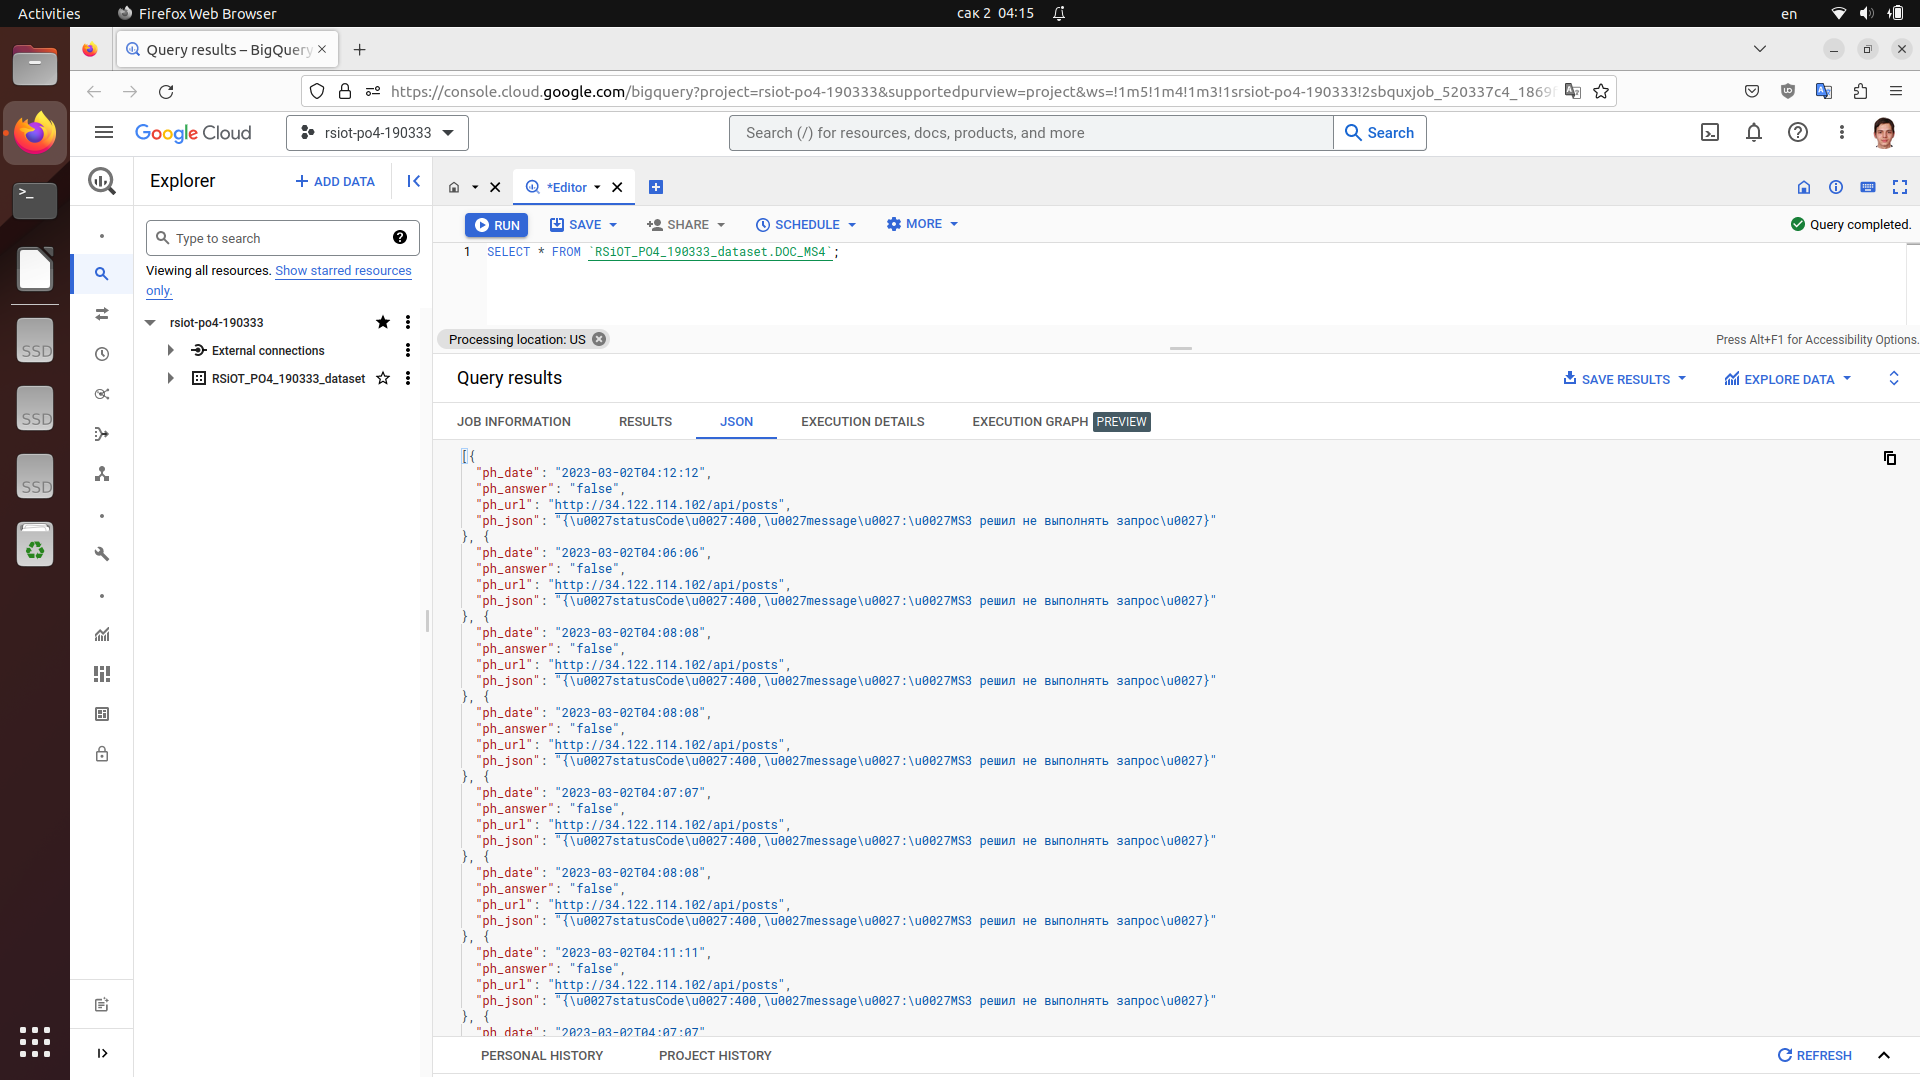
\includegraphics[width=16cm]
    {images/GoogleCloudBigQueryExplorer/2023-03-02_04-15-46.png}
    \caption{\_}
    \label{fig:41}
  \end{figure}

  \paragraph{} \textbf{Вывод}:
  Написали функцию (Google Cloud Functions), которую можно вызвать по ссылке,
  которая стучится на MS2 и записывает результаты в таблицу BigTable и таблицу BigQuery.
  Написали запланированую работу (Google Cloud Scheduler), которая вызывает функцию по ссылке каждую минуту.
  Создали сервисные аккаунты и получили от них приватный ключ от BigTable и BigQuery,
  чтобы в коде NodeJS можно было работать с таблицами от моего аккаунта.
  Сделали выборку данных из Google Cloud BigQuery.

  % = = = = = = = = = = = = = = = =
  % \newpage
  \begingroup
    \phantomsection
    \addcontentsline{toc}{section}{СПИСОК ИСПОЛЬЗОВАННЫХ ИСТОЧНИКОВ}
    \section*{Список использованных источников} %\section*{СПИСОК ИСПОЛЬЗОВАННЫХ ИСТОЧНИКОВ}

    \renewcommand{\addcontentsline}[3]{}% Remove functionality of \addcontentsline
    \renewcommand{\section}[2]{}% Remove functionality of \section

    \begin{thebibliography}{}

      \bibitem{GoogleCloudConsole}
      Getting started – Google Cloud console
      [Electronic resource]. -
      Mode of access:
      \url{https://console.cloud.google.com/getting-started}.
      Date of access: 02.03.2023.

      \bibitem{GoogleCloudBigTable}
      Bigtable – Google Cloud console
      [Electronic resource]. -
      Mode of access:
      \url{https://console.cloud.google.com/bigtable/instances}.
      Date of access: 02.03.2023.

      \bibitem{GoogleCloudServiceAccounts}
      Service accounts – IAM \& Admin – Google Cloud console
      [Electronic resource]. -
      Mode of access:
      \url{https://console.cloud.google.com/iam-admin/serviceaccounts}.
      Date of access: 02.03.2023.

      \bibitem{GoogleCloudFunctions}
      Functions – Cloud Functions – Google Cloud console
      [Electronic resource]. -
      Mode of access:
      \url{https://console.cloud.google.com/functions/list}.
      Date of access: 02.03.2023.

      \bibitem{GoogleCloudScheduler}
      Jobs – Cloud Scheduler – Google Cloud console
      [Electronic resource]. -
      Mode of access:
      \url{https://console.cloud.google.com/cloudscheduler}.
      Date of access: 02.03.2023.

      \bibitem{GoogleCloudBigQuery}
      BigQuery – Google Cloud console
      [Electronic resource]. -
      Mode of access:
      \url{https://console.cloud.google.com/bigquery}.
      Date of access: 02.03.2023.

    \end{thebibliography}
  \endgroup
  % = = = = = = = = = = = = = = = =
\end{document}
